\documentclass[oneside]{dissertation}

\usepackage[version=4]{mhchem}
\usepackage{siunitx}
\usepackage{pdflscape}
\usepackage{enumitem}
\usepackage[final]{pdfpages}
\usepackage{booktabs}
\usepackage{longtable}
\usepackage{multirow}
\usepackage{setspace}
\usepackage{nameref}
%\usepackage{cleveref}       % smart cross-referencing
\usepackage{xfrac}
\usepackage{algorithm2e}
\usepackage{subfig}
\usepackage[acronym,nonumberlist]{glossaries-extra}
\setabbreviationstyle[acronym]{long-short}
\makeglossaries
% \usepackage[parfill]{parskip}

\theoremstyle{definition}
\newtheorem*{objective}{Objective}
 
\theoremstyle{remark}
\newtheorem*{constraint}{Constraints}

\newcommand{\ra}[1]{\renewcommand{\arraystretch}{#1}}
 
\newcommand{\compresslist}{
	\setlength{\itemsep}{1pt}
	\setlength{\parskip}{0pt}
	\setlength{\parsep}{0pt}
	}
\onehalfspacing
%\doublespacing

\newcommand{\YJ}{Yellowjacket}
\newcommand{\GEM}{{\YJ}--GEM}

\DeclareSIUnit{\atmosphere}{atm}
\DeclareSIQualifier{\electric}{e}

\DeclareMathOperator*{\argmin}{arg\,min} % thin space, limits underneath in displays
\DeclareMathOperator*{\argmax}{arg\,max} % thin space, limits underneath in displays
%\DeclareMathOperator*{\argmin}{argmin} % no space, limits underneath in displays
%\DeclareMathOperator{\argmin}{arg\,min} % thin space, limits on side in displays
%\DeclareMathOperator{\argmin}{argmin} % no space, limits on side in displays

%%-------------------------------
%%  MATH MACROS
%%-------------------------------
\newcommand{\molesol}{\ensuremath{n_\lambda}}                               		% Moles of solution phase
\newcommand{\molestoich}{\ensuremath{n_\omega}}                             		% Moles of stoichiometric phase
\newcommand{\moleelem}[1]{\ensuremath{b_{#1}}}                              		% Moles of elements
\newcommand{\molefrac}[1]{\ensuremath{x_{#1(\lambda)}}}                     		% Mole fraction of solution phase species
\newcommand{\molespecies}[1]{\ensuremath{n_{#1(\lambda)}}}                  	% Moles of solution phase species
\newcommand{\stoich}[2]{\ensuremath{\nu_{#1#2}}}                            		% Stoichiometric coefficient
\newcommand{\cps}[1]{\ensuremath{\tilde{\mu}_{#1(\lambda)}}}               		% Chemical potential of solution phase species
\newcommand{\cpst}{\ensuremath{\tilde{\mu}_{\omega}}}                       		% Chemical potential of stoich. phase
\newcommand{\cpe}[1]{\ensuremath{\tilde{\Gamma}_{#1}}}                      		% Element potential
\newcommand{\pmgref}[1]{\ensuremath{\tilde{\mu}_{#1(\lambda)}^{\circ}}}     	% Partial molar reference Gibbs energy
\newcommand{\pmgrefst}{\ensuremath{\tilde{\mu}_{\omega}^{\circ}}}           	% Partial molar reference Gibbs energy of stoich. phase
\newcommand{\pmgid}[1]{\ensuremath{\ln{\molefrac{#1}}}}                     		% Partial molar ideal Gibbs energy of mixing
\newcommand{\pmgex}[1]{\ensuremath{\tilde{\mu}_{#1(\lambda)}^\text{ex}}}    	% Partial molar excess Gibbs energy of mixing
\newcommand{\sumsolnphase}{\ensuremath{\sum_{\lambda=1}^{\Lambda}}}         	% Summation solution phases
\newcommand{\sumstoichphase}{\ensuremath{\sum_{\omega=1}^{\Omega}}}         	% Summation stoich. phases
\newcommand{\sumelements}[1][j]{\ensuremath{\sum_{#1 = 1}^{C}}}             		% Summation elements
\newcommand{\sumspecies}[1][i]{\ensuremath{\sum_{#1 = 1}^{N_{\lambda}}}}    	% Summation species
\newcommand{\Residual}{\ensuremath{\boldsymbol{\epsilon}}}                  			% Residual vector
\newcommand{\Unknown}{\ensuremath{\mathbf{u}}}                              			% Unknown vector
\newcommand{\Jacobian}{\ensuremath{\mathbf{J}}}                             			% Jacobian
\newcommand{\Hessian}{\ensuremath{\mathbf{H}}}                              			% Hessian
\newcommand{\Constraint}{\ensuremath{\boldsymbol{\kappa}}}                  		% Constraint
\newcommand{\Step}{\ensuremath{\mathbf{s}}}                                 				% Newton step
\newcommand{\pder}[2]{\ensuremath{\frac{\partial #1}{\partial #2}}}                     		% First Partial derivative
\newcommand{\ppder}[2]{\ensuremath{\frac{\partial^2 #1}{\partial (#2)^2}}}              		% Second Partial derivative
\newcommand{\pqder}[3]{\ensuremath{\frac{\partial^2 #1}{\partial #2 \partial #3}}}      	% Second Partial derivative
\newcommand{\spder}[2]{\ensuremath{\sfrac{\partial #1}{\partial #2}}}                   		% First Partial derivative
\newcommand{\spqder}[3]{\ensuremath{\sfrac{\partial^2 #1}{\partial #2 \partial #3}}}   	% Second Partial derivative


\newabbreviation{calphad}{CALPHAD}{CALculation of PHAse Diagram}
\newabbreviation{mqm}{MQM}{modified quasichemical model}
\newabbreviation{mqmqa}{MQMQA}{Modified Quasichemcial Model in Quadruplet Approximation}
\newabbreviation{msr}{MSR}{molten salt reactor}

\begin{document}

%% Specify the title and author of the thesis. This information will be used on the title page (in title/title.tex) and in the metadata of the final PDF.

% Thesis Title
% Format: \title[Optional Subtitle]{Title}
\title[Development of Yellowjacket Gibbs Energy Minimiser]{Calculating Thermochemical Equilibrium for Multiphysics Simulations of Nuclear Materials} 

% Author Name
% Format: \author{Firstname}{Lastname}
\author{Parikshit}{Bajpai}

% Degree and Program
% Format: \DegreeProgram{Degree}{Program}
\DegreeProgram{Doctor of Philosophy}{Modelling and Computational Science}

% Thesis month and year
% Format: \DefenseDate{Date}{Month}{Year}
\DefenseDate{15}{November}{2022}

%% Use Roman numerals for the front matter.
\frontmatter

\begin{singlespace}
% Title page
\begin{titlepage}

%\begin{center}
%
%
%%% Extra whitespace at the top.
%\vspace*{2\bigskipamount}
%
%%% Print the title.
%{\makeatletter
%\CoverFont{b}{18}{20pt}\LARGE\@title
%\makeatother}
%
%%% Print the optional subtitle.
%{\makeatletter
%\ifx\@subtitle\undefined\else
%    \bigskip
%    \titlefont\titleshape\Large\@subtitle
%\fi
%\makeatother}
%
%\end{center}
%
%\cleardoublepage
\thispagestyle{empty}

\begin{center}

%% The following lines repeat the previous page exactly.

\vspace*{2\bigskipamount}

%% Print the title.
{\makeatletter
\CoverFont{b}{18}{20pt}\LARGE\@title
\makeatother}

%% Print the optional subtitle.
{\makeatletter
\ifx\@subtitle\undefined\else
    \bigskip
    \CoverFont{m}{12}{14pt}\Large\@subtitle
\fi
\makeatother}

%% Uncomment the following lines to insert a vertically centered picture into
%% the title page.
%\vfill
%\includegraphics{title}

%% Apart from the names and dates, the following text is dictated by the
%% promotieregelement.

\bigskip
\bigskip
\bigskip
\bigskip
\bigskip
\bigskip

by

\bigskip
\bigskip

%% Print the full name of the author.
\makeatletter
{\bf \@firstname\ {\@lastname}}
\makeatother

\bigskip
\bigskip
\bigskip
\bigskip

A thesis submitted to the\\
School of Graduate and Postdoctoral Studies\\
in partial fulfilment of the requirements for the degree of 

\bigskip
\bigskip
\bigskip
\bigskip

{\bf{\degree}}

% \medskip

in

%  \medskip

{\bf{\program}}

\bigskip
\bigskip
\bigskip
\bigskip

School of Graduate and Postdoctoral Studies 

\medskip

University of Ontario Institute of Technology (Ontario Tech University)

\medskip

Oshawa, Ontario, Canada

\medskip
\degreemonth{} \degreeyear

\vfill


\bigskip
\textcopyright{} \makeatletter \@firstname\ {\@lastname}\makeatother, \degreeyear


%\date{\today}

%% Extra whitespace at the bottom.
\vspace*{2\bigskipamount}

\end{center}

\end{titlepage}


% Thesis exam information

\cleardoublepage
\thispagestyle{plain}

%% The following line is dictated by the promotieregelement.
\begin{center}
\textbf{THESIS EXAMINATION INFORMATION}

\bigskip

Submitted by:  \makeatletter\textbf{\@firstname\ {\@lastname}}\makeatother

\bigskip
\bigskip

\textbf{\degree} in \textbf{\program}

\end{center}


\bigskip
\bigskip

\noindent \fbox{
    \parbox{\textwidth}{Thesis title: {\makeatletter\textbf{\@title}\makeatother}}
}

\bigskip

An oral defense of this thesis took place on \defensedate-\degreemonth-\degreeyear{} in front of the following examination committee:

\medskip

\noindent\textbf{Examining Committee:}

\bigskip

\begingroup
\renewcommand{\arraystretch}{2}
\begin{tabular}{lcl}
    Chair of Examining Committee &\phantom{Alphabet}& NAME \\
    Research Supervisor && NAME\\
    Research Co-supervisor && NAME \\
    Examining Committee Member && NAME \\
    Examining Committee Member && NAME \\
    Thesis Examiner && NAME, Affiliation (For Masters only)\\
    University Examiner && NAME \\
    External Examiner && NAME, Affiliation (For PhD only)\\
\end{tabular}
\endgroup

\medskip

\noindent The above committee determined that the thesis is acceptable in form and content and that a satisfactory knowledge of the field covered by the thesis was demonstrated by the candidate during and oral examination. A signed copy of the Certificate of Approval is available from the School of Graduate and Postdoctoral Studies.





\chapter*{Abstract}
\addcontentsline{toc}{chapter}{Abstract}
\setheader{Abstract}


Abstract goes here. Word limit 150 words Masters, 350 words PhD



\bigskip
\bigskip
\bigskip
\bigskip

\noindent \textbf{Keywords:} List up to 5 key terms separated by a semi-colon

\chapter*{Author's Declaration}
\addcontentsline{toc}{chapter}{Author's Declaration}
\setheader{Author's Declaration}


I hereby declare that this thesis consists of original work of which I have authored. This is a true copy of the thesis, including any required final revisions, as accepted by my examiners.


I authorize the University of Ontario Institute of Technology (Ontario Tech University) to lend this thesis to other institutions or individuals for the purpose of scholarly research. I further authorize University of Ontario Institute of Technology (Ontario Tech University) to reproduce this thesis by photocopying or by other means, in total or in part, at the request of other institutions or individuals for the purpose of scholarly research. I understand that my thesis will be made electronically available to the public.


<If this research work required approval of Research Ethics board(s), or the Animal Care Committee, add the following statement.>


The research work in this thesis that was performed in compliance with the regulations of Research Ethics Board/Animal Care Committee under \textbf{REB Certificate number/Animal care certificate file number.}


<Delete statement if this is not required.>

\bigskip
\bigskip

\makeatletter\textbf{\@firstname\ {\@lastname}}\makeatother

\chapter*{Statement of Contributions}
\addcontentsline{toc}{chapter}{Statement of Contributions}
\setheader{Statement of Contributions}


As of May 2018, all theses and dissertations are required to have a Statement of Contributions, which appears immediately before the Table of Contents. The Statement of Contributions must indicate the unique contributions of the author in the context of collaborative research that may have involved others who worked on various parts of the research described in the thesis. Types or contributions can include identification and design of the research project, performance of various parts of the research, and data analysis. In addition, if any parts of the thesis research have been published as an article, or is under consideration for publication, then the publication information must also be included here. 

\textbf{Example 1}

The work described in Chapter 4 was performed at the Futuristic Automotive Research Centre of Excellence (FARCE) in Hill Valley, California, using the Flux Capacitor testing laboratory operated by Dr. Emmett Brown. I was responsible for installing and testing flux capacitors in my automotive prototype vehicles.

\textbf{Example 2}

Part of the work described in Chapter 5 has been published as:

J.T.S. Allan, L.E. Prest, E.B. Easton, “The sulfonation of polyvinyl chloride: Synthesis and characterization for proton conducting membrane applications”, Journal of Membrane Science, 489 (2015) 175-182. doi: 10.1016/j.memsci.2015.03.093. 

I performed the majority of the synthesis, testing of membrane materials, and writing of the manuscript. 

\textbf{Example 3 – sole authorship}

I hereby certify that I am the sole author of this thesis and that no part of this thesis has been published or submitted for publication.  I have used standard referencing practices to acknowledge ideas, research techniques, or other materials that belong to others.  Furthermore, I hereby certify that I am the sole source of the creative works and/or inventive knowledge described in this thesis.

\chapter*{Acknowledgements}
\addcontentsline{toc}{chapter}{Acknowledgements}
\label{acknowledgements}

I am greatly thankful to Prof. Markus Piro for his constant guidance and support and for giving me the opportunity to work on this project. I am also grateful to the members of my candidacy examination committee, Professors Edward Waller, Lennaert van Veen, Hendrick de Haan and Kirk Atkinson. I appreciate your willingness to be on the committee and look forward to your suggestions and remarks.

I also appreciate Dr. David Andr\v{s} from Idaho National Laboratory and Prof. Michael Tonks from University of Florida for their help and support in the development of Yellowjacket. I'd also like to acknowledge Drs. Rich Martineau and David Andersson of Idaho National Laboratory and Los Alamos National Laboratory, respectively, for their role in facilitating this effort.

This work was funded by the Department of Energy Nuclear Energy Advanced Modeling and Simulation program under Contract No. DE-AC07-05ID14517 with the US Department of Energy. This research made use of the resources of the High-Performance Computing Center at Idaho National Laboratory, which is supported by the Office of Nuclear Energy of the U.S. Department of Energy and the Nuclear Science User Facilities under Contract No. DE-AC07-05ID14517. 

This research was undertaken, in part, thanks to funding from the Canada Research Chairs (950-231328) program of the Natural Sciences and Engineering Research Council of Canada.




\cleardoublepage
\tableofcontents

\cleardoublepage
\listoffigures

\cleardoublepage
\listoftables

\cleardoublepage
\listofalgorithms
\addcontentsline{toc}{chapter}{List of Algorithms}
\setheader{List of Algorithms}

% \cleardoublepage
\printglossaries

\end{singlespace}

%% The (optional) dedication can be used to thank someone or display a significant quotation.
 \dedication{\epigraph{Thermodynamics is a funny subject. The first time you go through it, you don't understand it at all. The second time you go through it, you think you understand it, except for one or two small points. The third time you go through it, you know you don't understand it, but by that time you are so used to it, it doesn't bother you any more.}{Arnold Sommerfeld}}

%% Use Arabic numerals for the page numbers of the chapters.
\mainmatter

%% Turn on thumb indices.
%\thumbtrue

\chapter{Introduction} \label{chap:introduction}

%==============================================================================================================================
%											Challenges Nuclear Material Design
%==============================================================================================================================	

Over the years, nuclear science and technology has made many positive contributions towards improving the quality-of-life of millions of people. Nuclear provides the world's second-largest source of low-carbon energy but it also helps control the spread of diseases, assists in diagnosis and treatment of cancer, powers space exploration missions, and drives the advancement of industry, agriculture and technology. Nuclear energy is not only at the core of world's sustainable development efforts but is also poised to take on an even bigger role as the world collectively moves to decarbonise many hard-to-abate sectors of the economy. 
%Recent years have seen a rapid shift in the engineering design of materials. Modelling and simulation have become essential tools in this context and are moving towards a multiscale, multiphysics approach where various physical phenomena  are coupled to enhance the accuracy of predictions. Of particular interest in this regard is the increasing desire to couple thermodynamics codes with other multiphysics codes such as phase field, fuel performance codes, etc. This chapter provides a brief background to the proposal and presents the motivation behind the proposed work.

%\section{Introduction}
%	Global population and per capita energy consumption are rising and electrical power generation not only plays a key role in the advancement of industry, agriculture, technology and the quality of living but is also an important measure of a country's economic development, power and independence. The global energy consumption has had significant impact on the environment in terms of greenhouse gas emissions and degradation of the quality of air, water and land.  As the call for action on climate change has become more pronounced and more urgent, there have also been concerns about energy security resource sustainability and human health. This has generated a renewed interest in nuclear energy as a source of reliable, low carbon footprint electricity source.

	As of 2022, around 440 nuclear plants around the world supplied \SI{2653}{\tera\watt\hour} of electricity, around 10\% of the world's total electricity \cite{WNA:2019aa}. Despite the strong support for, and growth in, intermittent renewable electricity sources in recent years, the fossil fuel contribution to power generation has remained virtually unchanged over the last decade and a half \cite{WNA:2019aa}. In its World Energy Outlook 2021, the Organisation for Economic Co-operation and Development (OECD) International Energy Agency (IEA)  has proposed an ambitious \emph{Sustainable Development Scenario} consistent with the goals clean and reliable energy and a reduction of air pollution, among other aims. In the scenario, by year 2050, nuclear based electricity generation should increase by 75\% to \SI{4714}{\tera\watt\hour}, a  capacity growth to \SI{669}{\giga\watt\electric} \cite{IEA:2018aa}. Key to a sustained growth of nuclear power is demonstrating their safety, reliability and economy.
	
	Though many nations across the globe, both industrialised and developing, are confident of the potential of nuclear energy, several challenges related to sustainability, reliability, economic competitiveness, safety, risk of proliferation, anticipated future needs beyonds electricity, and need for government support  remain \cite{GIF:2009aa}. To meet these challenges and develop future nuclear energy systems, the Generation {IV} International Forum (GIF) is undertaking necessary research and development to develop the next generation of innovative nuclear energy systems that can supplement today's nuclear plants and transition nuclear energy into the long term \cite{GIF:2019aa}. While promising in terms of sustainability, economics, safety and reliability, and proliferation resistance and physical protection, the Gen-{IV} nuclear reactors pose unique challenges in terms of engineering design, modelling and construction of these reactors. The design issues are themselves quite complicated and span a wide array of knowledge domains such reactor physics, chemistry, materials science, fluid flow and heat transfer, etc. Safe and economical operation of any nuclear system relies heavily on the success of nuclear fuels and structural materials which must operate under extreme environments. Compared to current generation of reactors, advanced reactors will operate at higher temperatures, under higher irradiation, at higher pressures, and in some cases, like Molten Salt Reactors (MSRs), with fluids that present more challenging corrosion problems \cite{Allen:2010aa}.

	
\section{Material Challenges in Nuclear Systems}

\section{CT in Nuclear}

MSR - Chemistry is very important, fuel salt composition (TC is imp here), corrosion, etc. PIRT Holcomb.

\section{Modelling and Simulation}
	The environment in a nuclear reactor induces complex multiphysics phenomena in nuclear materials, occurring over distances ranging from inter-atomic spacing to meters, and times scales ranging from microseconds to years. This multiphysics behaviour is often tightly coupled and many important aspects are inherently multidimensional  \cite{WILLIAMSON2012149}. Once in the reactor, nuclear materials are subjected to extreme radiation environments that continuously alter their thermo-mechanical properties \cite{STAN200920}. Moreover, due to irradiation effects, the physics and chemistry of such materials become more complicated over time. The safe and reliable performance of nuclear power plants requires choice of suitable materials and the assessment of long-term materials damage.

	Modern materials, including nuclear materials are developed using a combination of discovery, which involves evaluating existing materials to identify candidates with desirable properties, and design, which aims at  creating new materials with predefined qualities \cite{STAN200920}. While the traditional approach to discovery and design of materials was almost entirely experimental, recent developments in modelling and high performance computing has resulted in a much stronger collaboration and integration among theory, experiments and computational science. Multiscale, multiphysics models and simulations enable investigations over  a wide range of length and time scales which would otherwise be unfeasible using only experiments. Thus, computational models help augment and guide experimental campaigns and support economical discovery and design of materials within reasonable lead times.

	With material issues ranging from creep, swelling, fracture, fatigue to corrosion, impurity  effects and correlation between nano and microstructural scale, it is evident that a multiscale approach is required for a fundamental understanding of all the relevant phenomena. However, due to significant limitations on availability of computing resources, a majority of materials modelling and simulation efforts in the past adopted an operator splitting approach wherein the various physical phenomena were disconnected from each other. Though these methods were suitable for previous generation of nuclear reactors, addressing the materials challenges for advanced reactors requires a tightly coupled multiscale, multiphysics approach.

	\begin{figure}[htbp]
		\centering
		\includegraphics[width=0.75\textwidth]{figures/chapter-1/Multiphysics.pdf}
		\caption[Multiscale methods used for materials modelling simulation]{Multiscale theoretical and computational methods used for materials model development and computer simulation \cite{STAN200920}.}
		\label{fig:multiphys}
	\end{figure}

	Traditionally, nuclear material modelling has focussed on the macroscale behaviour of the materials. Such models rely on the principles of thermo-mechanics and are heavily rooted in experimental observations. For example, nuclear fuel behaviour is often modelled as a solid mechanics problem coupled with conductive heat transfer and fission gas release wherein the material properties are often either assumed to be constant or described using simplified models based on empirical correlations. Recently, there has been an impetus on atomistically informing mesoscale  and macroscale methods by optimising characteristic parameters of these scales against the output of atomistic calculations \cite{STAN200920}. Since such an approach is rooted in fundamental principles, the transfer of information between scales, through characteristic parameters such as density, energy, temperature, etc., results in a much more accurate description of material behaviour. Some of the theoretical and computational methods used in multiscale approach have been shown in figure~\ref{fig:multiphys}.

	\subsection{Corrosion in materials}
	Many emerging nuclear technologies, such as the Molten Salt Reactors (MSR), use high temperature fluids, such as molten fluoride/chloride salts, which lead to corrosion of the metal containment leading to problematic behaviours during the reactor operations. Corrosion in molten salts is a fundamentally different process from that in conventional applications, and most of the methods to control corrosion developed over previous centuries are of limited value \cite{Yoshioka:2017aa}. In fluoride salts, the protective oxide layer on alloys typically relied upon for high-temperature corrosion resistance dissolves, thereby exposing the fresh alloy surface to the molten salt. In molten chloride salts, passivity has been observed; however, the oxide layer is prone to attack and may not provide the necessary corrosion protection \cite{Sridharan:2013aa}. The corrosion process is accelerated by the impurities present in the salt and enhanced further by the presence of dissimilar metals due to activity-driven corrosion. Another issue to be considered is the mass transfer of corrosion products from hotter sections of the nuclear reactor and subsequent deposition in the colder areas that can clog the heat exchanger systems. Therefore, effectively predicting corrosion and related phenomena like leaching and deposition requires a multiscale, multiphysics approach \cite{Mcmurray:2018aa}.

	Corrosion is an electrochemical process composed of oxidation and reduction reactions, which are defined by the thermodynamics and kinetics of the system. While thermodynamics controls whether or not a material may corrode, kinetics influences how quickly the material will corrode. This corrosion behaviour is also significantly affected by the material microstructure and predicting corrosion therefore requires a multiphysics approach that can couple quantitative electrochemistry models of corrosion and chemical reactions with thermochemical equilibrium computations.

	\subsection{Thermodynamic modelling of materials}
	The phase and chemical behaviour of nuclear materials is governed by the thermochemical equilibrium state. While in many systems, equilibrium is often not achieved due to transport and/or chemical kinetics phenomenon, a thorough understanding of both transport and chemical evolution, and subsequently material properties, is  based on an accurate representation of thermochemical equilibria \cite{Devanathan:2010aa}. As an example, the oxygen chemical potential acts as the driving force for transport of oxygen in oxide fuels but a determination of these chemical potentials is impossible without determining the stable phases which depends on the oxygen-to-metal ratio which in turn is a function of burnup.  In the specific context of corrosion modelling, the difference in the free energy of the salt fluoride/chloride constituents and the fluorides/chlorides of the alloying elements is a key driving force for corrosion. For closed systems, the equilibrium concentration of the corrosion product fluorides/chlorides in the salt melt dictates the maximum extent of corrosion and is important in the long-term corrosion of containment materials. Therefore, thermodynamic equilibrium calculations play an important role in the context of corrosion modelling in advanced reactors.

	Capturing thermodynamic equilibria in multiphysics codes has traditionally relied on empirical correlations and the interest in direct coupling of thermodynamic equilibrium codes with multiphysics model is only a recent trend. While the empirical correlations do not convey the high fidelity of original thermodynamic analysis, performing thermodynamic equilibrium analysis within multiphysics codes is normally a very complex process and can significantly impede the computational performance of such codes. However, the recent developments in high performance computing have enabled the incorporation of these calculations which are of ever more importance in the discovery and design of materials for advanced reactors.

	The inputs for a thermodynamic equilibrium calculation are shown in figure~\ref{fig:Thermod}. Since thermodynamic equilibriums are isothermal and isobaric in nature, temperature and pressure are required as inputs along with the elemental composition of the material. While the equilibrium calculations are mathematically rigorous they do require thermodynamic models of materials to describe some parameters.  These thermodynamic models are generally developed using the Calculation of Phase Diagram (CALPHAD) approach shown in figure~\ref{fig:calphad}, which combines experimental and theoretical information to describe the thermodynamic properties through the Gibbs energy, applying a mathematical model containing adjustable parameters \cite{Lukas07}.  The multiscale approach also allows \textit{ab initio} molecular dynamics calculations to inform and improvise the thermodynamic models developed using the CALPHAD approach.
	\begin{figure}
        		\centering
        		\includegraphics[width=0.75\textwidth]{figures/chapter-1/Thermodynamics.pdf}
        		\caption{Input and output parameters of thermodynamic equilibrium calculations.}
        		\label{fig:Thermod}
    	\end{figure}

Figure~\ref{fig:Thermod} also shows some of the outputs produced by thermodynamic equilibrium calculations. The main outputs include the phase assemblage, i.e. the number of moles of phases present at equilibrium and the mole fraction of the species in those phases. The equilibrium calculations also provide the Gibbs energy of the system, the chemical potentials of the species, etc. These quantities are useful in multiphysics calculations where, for example, the chemical potential of oxygen can be used to model oxygen diffusion in a \ce{UO2} nuclear fuel pellet.
	\begin{figure}[htbp]
	\centering
	\includegraphics[width=0.5\textwidth]{figures/chapter-1/Calphad_method}
	\caption[Principle of CALPHAD method]{Principle of CALPHAD method by Zinkevich \cite{Zinkevich:2003aa}}
	\label{fig:calphad}
	\end{figure}

\section{Multiphysics Object Oriented Simulation Environment}
	The  Multiphysics Object-Oriented Simulation Environment {(MOOSE)} is a tool for solving complex coupled multiphysics equations using the finite element method. {MOOSE} uses an object-oriented design to abstract data structure management, parallelism, threading and compiling while providing an easy to use interface targeted at engineers that may not have a lot of software development experience. {MOOSE} provides extreme scalability and flexibility when compared to other finite element method (FEM) frameworks. For instance, {MOOSE} has the ability to run extremely complex material models, or even third-party applications within a parallel simulation without sacrificing parallelism. This capability is in contrast to what is often seen in commercial packages, where custom material models can limit the parallel scalability, forcing serial runs in the most severe cases \cite{gaston2015physics,moose-web-page}.

	The design goal of {MOOSE} is to give developers ultimate control over their physical models and applications. Designing new models or solving completely new classes of problems is accomplished by writing standard C++ source code within the framework's class hierarchy. Scientists and engineers are free to implement completely new algorithms using pieces of the framework where possible, and extending the framework's capabilities where it makes sense to do so. Commercial softwares do not have this capability, and instead opt for either a more rigid parameter system or a limited application-specific metalanguage \cite{moose-web-page}.

	Currently, apart from a number of other applications, such as {RELAP} \cite{Zhang:aa} for system level thermal hydraulics, {Rattlesnake} \cite{Wang:aa} for neutronics, etc., the {MOOSE} framework consists of two main applications for materials applications - the macroscale fuel performance code {Bison} \cite{Newman09} and the mesoscale phase field code {Marmot}  \cite{Tonks12}. Together, {MOOSE}, {Bison}  and {Marmot}, form the Fuels Product Line (FPL) to deliver an integrated set of increasingly predictive computational tools for nuclear fuel performance analysis and design. The FPL enable multiscale modelling and simulation of nuclear fuels where simulations of fuel performance at the engineering scale are informed by material property and behaviour models developed from mesoscale simulations of microstructure evolution under irradiation, which are themselves guided and enabled by inputs of fundamental materials parameters obtained from atomistic simulations. The multiscale, multiphysics approach allows an unprecedented degree of predictability of nuclear fuel performance.

	\subsection{Bison}
	The simulation of nuclear reactor fuel performance involves complex thermomechanical processes between fuel pellets, made of fissile material, and the protective cladding barrier that surrounds the pellets. {Bison} is an engineering scale code developed to predict the nuclear fuel performance under normal, off-normal, and accident conditions. By using highly efficient computational methods, {Bison} enables three dimensional, fully coupled multiphysics simulations on high fidelity geometric representations of fuel pins/pellets. {Bison} has been designed to be highly scalable and does not require the use of operator splitting, staggered or predictor-corrector approaches \cite{WILLIAMSON2012149}.

	Within the multiscale framework, {Bison} can be coupled with both mesoscale microstructure evolution tool {Marmot} as well as reactor core and system tools being developed under the Reactor Products Line to perform full scale simulations of the entire nuclear reactor. Coupling with {Marmot} allows {Bison} to easily and continuously incorporate new mechanistic, physics-based models produced by the mesoscale model development activities in order to extend its predictive capability to new fuels and operational regimes. While focussed on Light Water reactor (LWR) fuel, {Bison} is applicable to variety of fuel forms including the spherical TRISO fuel design \cite{NEAMS}.

	\subsection{Marmot}
	Due to its simple concept and large range of applicability, the phase field approach is a popular and powerful tool to model microstructure and has been applied in problems such as grain boundary migrations, martinistic transformation, two-phase flow, etc. The phase field approach treats all material interfaces as diffuse by representing structural features with continuous variables which smoothly transition from one value to another. Thus, phase field method not only eliminates the need to explicitly discretise boundaries and interfaces, it also enables describing microstructure through a system of partial differential equations.  The {Marmot} phase field framework has been developed to enable simulations of the microstructure evolution of nuclear fuels and materials under irradiation. By exploiting the object-oriented architecture of {MOOSE}, {Marmot} allows easy coupling of phase field with additional physics such as solid mechanics or heat conduction, to effectively predict the microstructural evolution at mesoscale. This allows prediction of evolution of material properties of nuclear materials under irradiation and can be used to inform engineering scale simulations and reduce the dependence of such simulations on empirical correlations. As a result, the multiscale framework can achieve true predictability even in compositional and operational regimes where little or no experimental data exists.

	Despite the wide ranging capabilities of the FPL, there remains a gap in terms of modelling advanced nuclear reactors. The high temperature operations of reactors such as the Molten Salt Reactors (MSR), which use molten fluoride/chloride salts as the fuel and coolant, produce a conducive environment for corrosion. The current FPL lacks a tool for corrosion modelling at microstructure scale and efforts are underway to develop a new {MOOSE} based application called {Yellowjacket} to bridge this gap.

	\subsection{Yellowjacket}
	{Yellowjacket} is a mesoscale framework for thermodynamics based modelling of corrosion in advanced reactor materials. Currently under development, it is a {MOOSE} based application that couples quantitative models of corrosion with thermodynamic equilibrium and chemical kinetics models to predict the rate of material loss, corrosion product production and precipitate production in advanced nuclear reactors. {Yellowjacket} relies on phase field models for structure evolution, coupling it with Poisson equation for electrostatics, fracture models and thermochemical equilibrium solvers to provide a holistic environment for corrosion modelling and simulation. As shown in figure~\ref{fig:yjmoose}, {Yellowjacket} depends on the {MOOSE} framework for the development infrastructure and follows the Nuclear Quality Assurance Level 1 (NQA 1) \cite{NQA-web-page} development process.

	\begin{figure}[htbp]
		\centering
		\includegraphics[width=0.75\textwidth]{figures/chapter-1/Yellowjacket_MOOSE.pdf}
		\caption{Illustration showing the underlying interface provided by {MOOSE} and the physics modules of {Yellowjacket}.}
		\label{fig:yjmoose}
	\end{figure}

	{Yellowjacket} is being developed through a joint collaboration between the Nuclear Fuels and Materials Group at Ontario Tech University, University of Florida, Idaho National Laboratory and Los Alamos National Laboratory, and is funded primarily by the United States Department of Energy (US-DOE) through the Nuclear Energy Advanced Modelling and Simulation (NEAMS) program.

	This thesis is aimed at developing a thermodynamic equilibrium solver for the corrosion modelling tool {Yellowjacket} and the goals of this research are specified in the following chapter. The phase field component of {Yellowjacket} is being investigated by another PhD student at University of Florida.

\chapter{Statement of Work} \label{chap:overview}
	
\section{Problem Statement}
    Thermodynamic equilibrium calculations are key to providing material properties and boundary conditions in multiphysics simulations. For advanced reactors such as MSRs, there's a need to replace empirical material properties with calculations rooted in fundamental laws of thermodynamics.  Despite the growing interest in direct coupling of thermodynamic equilibrium, the MOOSE framework lacks a tool for such calculations.

    While several equilibrium thermodynamics codes already exist, the rationale behind developing a new equilibrium thermodynamics code lies in the numerous limitations of these pre-existing tools. All but a handful of these codes are standalone codes aimed at single calculations, phase diagram generation and database development. Moreover, these codes usually support only a small number of system components. Among the codes that do exist with the capability of handling large systems and are aimed at multiphysics simulations, there are still several drawbacks and they do not meet many requirements of the MOOSE framework. These drawbacks include unavailability of readily available API for coupling to MOOSE apps and lack of SQA standards. Thus, a new equilibrium thermodynamics solver needed to be developed.

\section{Objective}
    The overarching objective of this work was to incorporate native computational thermodynamics capabilities into the multiphysics framework MOOSE through the development of a new state-of-the-art equilibrium thermodynamic solver called \GEM. The software consolidates and integrates years of advancements and research in computational thermodynamics and leverages state-of-the-art nonlinear equation solvers and optimisation algorithms to enable real-time thermodynamic property calculation in multiphysics simulations. 

\section{Challenges}
    There are several challenges that had to be addressed in order to achieve the aforementioned objective.
    \begin{enumerate}
        \item Several thermodynamic models are used for representing the Gibbs energies of phases. Many models, in particular the modified quasichemical model in quadruplet approximation (MQMQA), are not well understood and the details required for implementing them in a solver are not readily available.
        \item Thermodynamic calculations are inherently very expensive and the computational cost increases very rapidly with the number of system components. In fact, the cost  scales cubically $\left(\mathit{O}\left(C^3\right)\right)$ with the number of system components $C$ and the choice of algorithms can significantly impact the calculation time. This can be prohibitive in multiphysics simulations.
        \item Equilibrium calculations require solving a non-convex global optimisation problem. The algorithms used in literature are either primitive or limited to relatively very simple problems. This can affect both performance and reliability of the solver which is critical considering the intended application.
        \end{enumerate}

\section{Tasks}
    The work was split into a series of tasks aimed at navigating the challenges to achieve the objective. These tasks also highlight the main contributions of this work:
    \begin{itemize}
        \item Analyse several thermodynamic models used to describe nuclear materials and derive the chemical potential expressions required for implementing the models in the code. See \nameref{chap:thermo}.
        \item Critically survey the numerous algorithms used for thermodynamic equilibrium calculations and identify the solution approach to be adopted. Identify key software design choices and optimise the algorithms for implementation in {\GEM}. See \nameref{chap:equilibrium} and \nameref{chap:implementation}.
        \item Develop the new equilibrium solver in C++ following MOOSE coding conventions. The code must meet the rigorous source code control, continuous integration and verification requirements of MOOSE. Though {\GEM} is not NQA-I certified, it must try to achieve same quality standards as MOOSE is NQA-I certified. See \nameref{chap:implementation}.
        \item Quantitatively compare various global optimisation algorithms available in literature, and, based on performance and reliability, select and implement the algorithm {\GEM}. See \nameref{chap:implementation}.
        \item Demonstrate the capabilities of the developed thermodynamic solver through potential applications and benchmark against results available in literature and through other codes. See \nameref{chap:results}.
        \item An internship at Idaho National Laboratory from June 2021 to September 2022, working on MOOSE integration of \GEM. Owing to COVID-19 induced travel restrictions, this internship was virtual.
    \end{itemize}

\section{Deliverables}
	The outcomes of this research were documented in several ways including publications in peer-reviewed journals, conference presentations and annual progress reports submitted to the Idaho National Laboratory (INL). The main deliverables of this work were as follows:
	\begin{enumerate}
	\item Code base for {\GEM} delivered to INL via export controlled repository on Nuclear Science User Facility (NSUF) High Performance Computing (HPC)'s GitLab instance. Since {\YJ} is export controlled, the code has not been shared here.
	\item Four annual progress reports submitted to INL in September 2019, September 2020, August 2021 and September 2022. 
	\item Six publications in peer-reviewed journals and seven conference presentations and posters. See \nameref{publications}.
	\end{enumerate}
	
\chapter{Computational Implementation} \label{chap:implementation}


	This chapter presents the numerical algorithms that can be employed in computing thermodynamic equilibria. While most of these algorithms embody the concepts previously presented in the open literature, there remains a scope for improving the efficiency and capabilities of some of these algorithms through careful implementation and/or building upon them. This chapter discusses the computational implementation of the proposed thermodynamic equilibrium solver, the top-level architecture of which has been outlined in figure~\ref{fig:structure}. The program essentially consists of a parsing and input module to read the required thermodynamic data and system information followed by initialisation routines which provide the initial assemblage to a non-linear GEM routine. The assemblage from the non-linear solver is then checked to ensure global minimum is achieved at which stage the outputs are produced.
	\begin{figure}[htbp]
	 	\centering
	   	\includegraphics[width=0.65\textwidth]{figures/YJ_structure.pdf}
	   	\caption{Top-level architecture of the proposed thermodynamic equilibrium code.}
	   	\label{fig:structure}
	\end{figure}

\section{Opportunities for Novel Contributions}
Before delving into the details of a thermodynamic solver, a number of opportunities for novel contributions are presented here. The first and the foremost is integration of the thermodynamic solver within multiphysics framework \texttt{MOOSE}. \texttt{MOOSE} based applications currently leverage the thermochemistry library \texttt{Thermochimica} to perform thermodynamic equilibrium calculations. However, since \texttt{Thermochimica} was developed in FORTRAN and wasn't developed within the \texttt{MOOSE} framework, coupling it requires writing wrapper classes for every intended application. Not only does this lead to waste of time and resources, it also needs a lot of effort to maintain reliability and achieve desired performance. The new thermodynamic sover will be built within the \texttt{MOOSE} framework and will eliminate the need to write multiple wrapper classes. Furthermore, since it will use the same software quality assurance practices as \texttt{MOOSE}, it will be able to meet the desired performance standards.

	In addition to coupling, the development of the new thermodynamic code will try to achieve performance gain through advanced algorithm development. While the GEM method has little scope of improvement in itself, the performance of thermodynamic equilibrium codes can be significantly improved by improving the initialisation routines and focussing on strategies for updating the estimated phase assemblage. The strategies to achieve this goal have been presented in the following sections. Novel contributions can also be made towards global optimisation routines for thermodynamic equilibrium solvers. As shown in section~\ref{sec:opt_theory}, ensuring that a global minimum of Gibbs energy has been achieved is a challenging task and the global optimisation methods available in the literature have mostly been problem specific. Since a thermodynamic equilibrium solver needs to perform well for different kinds of problems, significant contributions can be made by implementing robust global optimisation algorithms. These strategies are discussed in the following sections.

\section{Parsing and Input}
	Calculation of thermodynamic equilibrium requires a thermodynamic database, which includes Gibbs energy expressions of the different phases and species that can exist in the system. These thermodynamic databases are developed using the well established CALculation of PHAse Diagrams (CALPHAD) method \cite{liu_wang_2016} and are available in different formats, the most commonly used being ThermoCalc (*.tdb) and ChemSage (*.dat) data file formats, which are generated by the commercial software ThermoCalc and FactSage, respectively. An example of a typical ChemSage data file is shown in figure~\ref{fig:datfile} and consists of a header block followed by information blocks for every possible phase in the system.
	\begin{figure}[htbp]
	 	\centering
	   	\includegraphics[width=\textwidth]{figures/NiKF.pdf}
	   	\caption{A marked-up example of a ChemSage data file of the \ce{Ni-K-F} system \cite{OcadizFlores18}}
	   	\label{fig:datfile}
	\end{figure}

	The data file parser for the thermodynamic equilibrium part of \texttt{Yellowjacket} has been developed in C++ and it performs the extraction of free energy expressions from *.dat thermodynamic database files (ChemSage format) and exports a list of free energy terms for each phase (or a user specified subset of phases). The data-file parser has the following capabilities:
\begin{itemize}
\itemsep-0.5em
    \item Extract system information from *.dat files and ensure that the data is consistent with the inputs and appropriate for consideration.
    \item Extract Gibbs energy terms for different phases and all the species within each phase.
    \item Store the Gibbs energy terms to ensure that terms corresponding to each phase can be selectively and conveniently retrieved.
\end{itemize}

	Another requirement for Gibbs energy minimisation is physical parameters of the system, namely, the temperature, pressure and composition. Within a multiphysics framework, these informations are required for each finite element at every time-step. In the context of the proposed Gibbs energy minimiser, the system inputs are provided by \texttt{MOOSE} which passes the information at the time the Gibbs energy minimiser is called. For standalone applications, this information can be provided as an input through the \texttt{MOOSE} input file.

\section{Initialisation}
	Much like any other optimisation problem, the choice of initial estimate plays a critical role in reducing the amount of computational time required for the solution to converge to a minimum. This need for providing initial estimates of the number of moles of phases and the mole fractions of the species in those phases creates a significant challenge. Many early softwares  created for the purpose of estimating thermodynamic equilibrium, for example SOLGASMIX, required the user to input an initial estimate. Providing such initial estimates relied on the intuition of the user and was often very inconvenient for the user, especially when working with complex systems and/or systems where finding estimates from intuition was not straightforward.
%	, it also left the door open to encountering an initial assemblage far from the actual, thus resulting in large computational costs.
	To overcome the need for the user to enter the initial estimates,  Eriksson and Thompson \cite{Eriksson89} proposed an initialisation algorithm called \textit{levelling} that has found widespread application in thermodynamic equilibrium softwares. Subsequently, Piro and Simunovic \cite{Piro12a} proposed the \textit{post-levelling} method as an extension to levelling in order to further improve the initial estimate.

	\subsection{Linear solver}
	The levelling algorithm was developed to accelerate the rate of convergence by eliminating the phases and species that have an insignificant contribution in the final phase assemblage. The algorithm is based on a temporary treatment of all species and phases in the system as pure stoichiometric phases. Mathematically, this amounts to temporarily converting the non-linear optimisation problem into a linear optimisation problem and the algorithm for the computational implementation has been illustrated in figure~\ref{fig:levelling}.
	\begin{figure}[htb]
		\centering
		\begin{tikzpicture}[auto,
    			block_center/.style ={rectangle, draw=black, thick, fill=white, text width=0.2\textwidth, text centered, minimum height=2em},
    			block_side/.style ={rectangle, draw=black, thick, fill=white, text width=0.2\textwidth, text centered, minimum height=2em},
			block_noborder/.style ={rectangle, draw=none, thick, fill=none, text width=0.15\textwidth, text centered, minimum height=0.5em},
			block_small/.style ={rectangle, draw=none, thick, fill=none, text width=0.1\textwidth, text centered, minimum height=0.5em},
			line/.style ={draw, thick, -stealth}]
    			% Outlining the flowchart using the PGF/TikZ matrix funtion
    			\matrix [column sep=0.15\textwidth,row sep=5em] {
      				{} & \node [block_center] (01) {Initial guess}; & {}\\
      				{} & \node [block_center] (11) {Calculate chemical potential of pure components}; & {}\\
      				\node [block_side] (20) {Initial estimate found}; & \node [block_center] (21) {Levelling}; & \node [block_side] (22) {Calculate molar amounts};\\
      				{} & \node [block_center,yshift=-1cm] (31) {Exchange phase}; & {}\\
      				{} & \node [block_center] (41) {Compare to the list of previous assemblages}; & \node [block_side] (42) {Calculate chemical potential of component};\\
    			};	% end matrix
    			% connecting nodes with paths
    			\begin{scope}[every path/.style=line]
      				\path (01) edge (11);
     				\path (11) edge (21);
      				\path (21) edge node[block_noborder,anchor=east]{\footnotesize{Phase with most negative relative Gibbs energy}} (31);
      				\path (31) edge (41);
      				\path (22) edge node[block_noborder,anchor=south]{\footnotesize{All positive and real}} (21);
      				\path (21) edge node[block_noborder,anchor=south]{\footnotesize{All phases' Gibbs energies are positive}} (20);
      				\path (41) edge node[block_noborder,anchor=north]{\footnotesize{New assemblage}} (42);
      				\path (42) edge (22);
      				\path[-] (22.185) edge node[block_noborder,rotate=49.5,anchor=south]{\footnotesize{Negative or non-real numbers}} (31.5);
      				\path[-] (41.10) edge[bend right=60] node[block_small,anchor=west,shift={(-0.125cm,0)}]{\footnotesize{Already considered}} (31.355);
     				\path[-] (42.135) edge[bend right=37] node[block_small,anchor=west,shift={(0,0.225cm)}]{\footnotesize{Non-real numbers}} (31.360);
    			\end{scope}
 		\end{tikzpicture}
  		\caption{Illustration of the levelling algorithm \cite{Loukusa:2014aa}}
  		\label{fig:levelling}
 	\end{figure}

	Since the Gibbs energy is a relative thermodynamic function and the Gibbs energies of each component element are not related to one another \cite{Eriksson89}, it is possible to numerically alter the Gibbs energy of each phase while preserving the elemental differences. Levelling is performed by representing the set of Gibbs energies relative to the collection of phases assumed to be most stable and uses a relative Gibbs energy function called the \textit{absolute Gibbs energy} by Eriksson and Thompson and is the Gibbs energy of the pure species per atom in the species as shown in equation~\eqref{eq:absGibbs}
	\begin{equation}\label{eq:absGibbs}
		\hat{G}_i = \frac{G_j}{\sum_{j=1}^C \nu_{ij}}
	\end{equation}

	The levelling process determines the combination of phases yielding the lowest Gibbs energy by evaluating a combination of Gibbs energies on a relative basis. A phase that has a negative relative Gibbs energy with respect to the assemblage indicates that a phase in the assemblage must be replaced by the current phase to achieve a lower integral Gibbs energy.

	Mathematically, levelling is achieved through an iterative process that systematically adjusts fixed combinations of phases, subject to the linear equality and inequality mass balance constraints, to progressively minimise the GIbbs energy of the system \cite{Piro12a}. At iteration $m+1$, the adjustment to be applied to the relative Gibbs energy of phase $i$ is defined by \cite{Eriksson89}:
	\begin{equation} \label{eq:lev_adj}
		\begin{aligned}
			d \hat{G}_i^{m\rightarrow m+1} &= \sum_{j=1}^{C} c_{i,j} d \Gamma_j^{m\rightarrow m+1}\\
			\hat{G}_i^{m+1} &= \hat{G}_i^{m} - d \hat{G}_i^{m\rightarrow m+1}
		\end{aligned}
	\end{equation}
	where, $c_{i,j}$ denotes the atomic fraction of element $j$ in species $i$ and $d \Gamma_j^{m\rightarrow m+1}$ is the adjustment applied to the chemical potential of element $j$, which in turn is determined by the most stable phases found at iteration $m$.

	In  matrix form, the overall mass balance constraint can be represented as \cite{Piro12a}
	\begin{equation} \label{eq:levMB_mat}
		\mathbf{A^T} \mathbf{n}= \mathbf{b}
	\end{equation}
	where $\mathbf{A} \in \mathbb{R}^{E \times \Phi}$ represents the stoichiometric matrix, $\mathbf{n} \in \mathbb{R}^{\Phi }$ denotes the column vector of the number of moles of each phase, and $\mathbf{b} \in \mathbb{R}^{E}$ is the column vector with the total mass of each element in the system. When equation~\ref{eq:levMB_mat} is used in levelling, $\Phi = E$.

	The initial guess for the levelling method is the most chemically stable form of each element and the stoichiometric matrix $\mathbf{A^T}$ in equation~\eqref{eq:levMB_mat} becomes a diagonal matrix. Subsequently, provided all elements of vector $\mathbf{b}$ are positive, all the elements of $\mathbf{n}$ must also be positive. However, the diagonality of the stoichiometric matrix is not preserved over subsequent iteration and it assumes a non-symmetric sparse form. In fact, the matrix $\mathbf{A^T}$ might become rank deficient if proper care is not taken while selecting the phase assemblage.

	In levelling, since the number of phases in the system is equal to the number of elements, the element potentials can then be uniquely determined from the current estimated phase assemblage by solving the following system of linear equations:
	\begin{equation} \label{eq:levEP_mat}
		\mathbf{A^T} \boldsymbol{\Gamma} = \boldsymbol{\mu}
	\end{equation}
	where $\boldsymbol{\Gamma} \in \mathbb{R}^{E} $ and $\boldsymbol{\mu} \in \mathbb{R}^{\Phi}$.

	The next step in levelling is updating the phase assemblage in accordance with equation~\eqref{eq:lev_adj}. A  species with a positive $\hat{G}_i^{m+1}$ would yield a thermodynamically less stable assemblage and is left out along with phases with insignificant contributions to final equilibrium while the phase with the most negative $\hat{G}_i^{m+1}$ is introduced into the assemblage by replacing a phase in the previous assemblage. The phase assemblage at this stage must meet three requirements. First, the number of moles of all phase in $\mathbf{n}$ must be non-negative and real. Second, all the elements of the vector $\boldsymbol{\Gamma}$ must be real. Finally, the phase assemblage must not have been previously considered. If the phase assemblage does not meet any of these requirements, the phase with the second lowest relative Gibbs energy must be considered, and so on.

	While the criteria for the phase to be added in the system was well established by Eriksson and Thompson, a criterion to select the phase to be replaced wasn't proposed and, typically, local iterations were performed to systematically traverse through the candidate phases until a particular combination yielded an entire set of non-negative and real mole numbers \cite{Eriksson89}. The number of these local iterations rapidly grows with the number of elements in the system and an alternative named \emph{Euclidean norm} was proposed by Piro and Simunovic \cite{Piro12a}. This method has been described in sec.~\ref{sec:Euclidean}

	Once the new phase has been exchanged with one of the existing phases and its acceptability has been determined, levelling step is repeated until no phases with negative absolute Gibbs energy remain in the system. At this stage, the assemblage can be passed on to a non-linear solver as the initial estimate.


	\begin{figure}[htbp]
		\centering
		\includegraphics[width=\textwidth]{figures/Levelling_illustration}
		\caption{Illustration of the levelling process for a binary system of \ce{U-O} at each iteration (1 \si{\mole} \ce{U}, 2.2 \si{\mole} \ce{O}, 298.15 \si{\kelvin}, 1 \si{atm}) \cite{Piro11b}.}
		\label{fig:lev_illus}
	\end{figure}

	An example of the levelling method is presented in figure~\ref{fig:lev_illus}. In the illustration, in the first iteration, the phase with the most negative Gibbs energy is paired with another phase that together has non-negative molar quantities. At the end of iteration 0, choosing solid \ce{UO2} as the phase with the most negative relative Gibbs energy and arbitrarily choosing solid \ce{UO3} to pair it with, the equivalent Gibbs energies of pure uranium and pure oxygen are computed and followed by the element potentials $\Gamma_{\ce{U}}$ and $\Gamma_{\ce{O}}$ (represented by the dashed red line). The levelling procedure is then applied and the relative Gibbs energies of the terms are calculated.

	At the start of iteration 1, the relative Gibbs energy of solid \ce{U3O8} is negative with respect to the combination of solid \ce{UO2} and solid \ce{UO3}, indicating it must be introduced in the assemblage. The internal linear solver then determines the phase that must be replaced and the iterative process continues with the updated phase assemblage.

	At the end of the levelling procedure, the assemblage has the lowest Gibbs energy with all other phases being positive with respect to the assemblage. The Gibbs energy of the pure stoichiometric system is thereby minimised. For the example presented in figure~\ref{fig:lev_illus}, the levelling solver converges in only 3 iterations. According to Eriksson and Thompson \cite{Eriksson89}, the computational expense using levelling can be up to two to five times lower than the general equilibrium calculations.

	Mathematically, the levelling  process always respects the Gibbs phase rule, mass balance and the Gibbs' criterion and the number of iterations required to achieve convergence is typically close to the number of elements. This results in significant computational advantage when considering exceeding large number of possible phase combinations as the number of elements in the system grow making levelling an excellent choice as an initialisation routine.

	\subsection{Post-levelling}
	Developed by Piro and Simunovic \cite{Piro12a}, the post-levelling method is an extension to the levelling method and can be used to refine the assemblage provided by the levelling method by accounting for the ideal mixing of the phases and relaxing the assumption that the phases are pure. Thus, post-levelling acts as an intermediate step between levelling and the non-linear solver. While post-levelling resembles the non-linear solver in the incorporation of compositional component in the chemical potential of the solution phase constituents, the primary distinction between them is that post-levelling considers only dominant phases identified by levelling as compared to the non-linear solver which considers all the constituents. Furthermore, the non-linear solver also considers non-ideal behaviour.

		The chemical potential term in post-levelling takes the following form:
		\begin{equation}
			\begin{aligned}
				\mu_{i(\lambda} &= g_{i(\lambda)}^0 + RT \ln{(x_{i(\lambda)})} \\
				x_{i(\lambda)} &= \frac{n_{i(\lambda)}}{\sum_{k=1}^{N_{\lambda}}n_{k(\lambda)}}
			\end{aligned}
		\end{equation}
		where $N_{\lambda}$ is the number of constituents in solution phase $\lambda$ identified by levelling and is less than the actual constituents in the phase. The element potentials can then be computed using equation~\eqref{eq:levEP_mat} and an iterative process similar to levelling can be followed.

		A demonstration of the post-levelling method in predicting the element potentials of combustion products from a coal fire shows that compared to levelling, post levelling calculations provide values much closer to the equilibrium values. As a result, the rate of convergence of the non-linear solver improves by a large factor.  While exact gains depend on the non-linear solver, line-search algorithm and the strategy for updating the estimated phase assemblage, relative performance gains can be easily envisaged even though post-levelling process incurs additional computational cost. This can be attributed to the fact that the cost of post-levelling is negligible in comparison to the cost of a single iteration in a non-linear solver \cite{Piro12a}.

	\subsection{Euclidean norm} \label{sec:Euclidean}
	The Euclidean norm method was proposed by Piro and Simunovic \cite{Piro12a}, to strategically rank the best candidate phases to accommodate a new phase change. The Gibbs phase rule requires that when the thermodynamic degree of freedom $F$ equals zero, a phase must be removed in order to introduce a new phase. Determining whether a candidate phase is feasible is the most expensive task within the global iteration cycles as it requires solution of a simultaneous equation to ensure that the Hessian matrix is non-singular \cite{Piro12a}. If there are multiple candidate phases, this iterative process must be repeated for each candidate.

	The Euclidean norm method systematically ranks the best candidates to be withdrawn from the system without having to perform an exhaustive search. The method is based on the principle that the best candidate phase to be withdrawn from the current assemblage has the most similar atomic composition to the phase that has to be added to the system.

	The atomic fraction of element $j$ in a pure stoichiometric phase $\omega$ is represented as:
	\begin{equation}
		c_{\omega,j} = \frac{c_{\omega,j}}{\sum_{k=1}^{E} x_{i(\omega)}\nu_{\omega,j}}
	\end{equation}

	Similarly, in the solution phase  $\lambda$, the atomic fraction of element $j$ is computed by
	\begin{equation}
		c_{\lambda,j} = \frac{\sum_{i=1}^{N_{\lambda}} \nu_{i,j}}{\sum_{i=1}^{N_{\lambda}} \sum_{k=1}^{E} x_{i(\lambda) \nu_{i,k}}}
	\end{equation}

	Denoting the atom fraction of the element $j$ in the new phase that is to be introduced into the system with $c_{\phi,j}^{*}$, the difference between this phase and the phases currently in the assemblage is given by the Euclidean norm of each phase $\phi$
	\begin{equation}
		\|c_\phi\|_2 = \sqrt{\sum_{j=1}^{E} \left(c_{\phi,j} - c_{\phi,j}^{*}\right)^2}
	\end{equation}

	The phase with the lowest Euclidean norm has the most similar composition to the phase to be introduced in the assemblage. In case the resulting assemblage does not meet the criterion to be a valid assemblage, the phase with the second lowest Euclidean norm can be introduced and so on.

	As shown in figure~\ref{fig:PEA_gains}, the overall computational expense of thermodynamic calculations is significantly reduced when post-levelling and Euclidean norm methods are utilised \cite{Piro12a}. These performance gains can offer a significant advantage when considering multiphysics simulations where thermodynamic equilibrium is often the most computationally expensive calculation.

	\begin{figure}[htbp]
		\centering
		\includegraphics[width=0.65\textwidth]{figures/PEA_Gains}
		\caption{Performance gains when employing post-levelling and Euclidean-norm algorithms \cite{Piro12a}.}
		\label{fig:PEA_gains}
	\end{figure}


	\subsection{Temporal series estimate}
	While in most cases levelling and post-levelling methods can provide initial assemblages close to the final assemblage, using the assemblage from a previous time step in multiphysics codes can often provide much closer estimates to the final assemblage. In time-dependent multiphysics simulations, this can result in significant performance gains as has been recently shown through the implementation of this strategy in \texttt{Thermochimica} \cite{Poschmann:2019aa}. These performance gains can be attributed to the fact that the convergence of the non-linear solver can be significantly accelerated by providing initial estimates close enough to the final assemblage. This temporal initialisation strategy has been illustrated in figure~\ref{fig:temp_init}
	\begin{figure}
		\centering
		\begin{tikzpicture}[auto,
    			block_center/.style ={rectangle, draw=black, thick, fill=white, text width=0.2\textwidth, text centered, minimum height=2em},
    			block_side/.style ={rectangle, draw=black, thick, fill=white, text width=0.2\textwidth, text centered, minimum height=2em},
			block_noborder/.style ={rectangle, draw=none, thick, fill=none, text width=0.2\textwidth, text centered, minimum height=0.5em},
			block_small/.style ={rectangle, draw=none, thick, fill=none, text width=0.1\textwidth, text centered, minimum height=0.5em},
			line/.style ={draw, thick, -stealth}]
    			% Outlining the flowchart using the PGF/TikZ matrix funtion
    			\matrix [column sep=0.15\textwidth,row sep=3em] {
      				\node [block_center] (00) {Start at initial time}; & {} & {}\\
      				\node [block_center] (10) {Levelling}; & {} & {}\\
				\node [block_center,yshift=-1cm] (20) {Non-linear solver}; &  \node [block_side,yshift=-1cm] (21) {Save assemblage in memory}; & \node [block_side,yshift=-1cm] (22) {Reinitialise with saved assemblage};\\
      				\node [block_side] (30) {Solution found}; & {} & {}\\
    			};	% end matrix
    			% connecting nodes with paths
    			\begin{scope}[every path/.style=line]
      				\path (00) edge (10);
     				\path (10) edge (20);
      				\path (20) edge node[block_noborder,anchor=east]{\footnotesize{Stop time reached}} (30);
      				\path (20) edge (21);
      				\path (21) edge node[block_noborder,anchor=south]{\footnotesize{Timestep}} (22);
      				\path[-] (22.90) edge[bend right] node[block_noborder,anchor=west,shift={(0.75cm,0.25cm)}]{\footnotesize{Temporal reinitialisation failed}} (10);
      				\path[-] (22) edge[bend right] (20);
    			\end{scope}
 		\end{tikzpicture}
  		\caption{Illustration of the temporal series initialisation algorithm.}
  		\label{fig:temp_init}
 	\end{figure}

	The details of the implementation of the temporal initialisation strategy in \texttt{Yellowjacket} have not yet been set in stone but, based on \texttt{Thermochimica} acceleration results obtained by Poschmann et al. \cite{Poschmann:2019aa} , a significant performance gain is foreseen which justifies the use of this strategy especially in coupled multiphysics problems where thermodynamic equilibrium calculations are impediment to significant performance gains. However, this might also lead to a drastic increase in memory requirement and a compromise must be made between  computing time gains and increased memory requirements.

	\subsection{Boundary value estimate}
	For the case where Gibbs energy minimisation is performed on a 2D/3D mesh, very good initial estimates can conceivably be provided to the non-linear solver by exploiting the results from the neighbouring solutions in space at the same time step. As an example, the final assemblage of element A on the finite element mesh shown in figure~\ref{fig:BV_Illustration} can be used as the initial assemblage for element B. This initialisation scheme relies on the principles of continuum between adjacent cells, i.e., if the mesh is sufficiently resolved, the difference between system potentials (temperature, pressure and chemical potentials) between two neighbouring cells must be small.
	\begin{figure}[htbp]
		\centering
		\includegraphics[width=0.35\textwidth]{figures/BV_FEM}
		\caption{Illustration of the boundary value initialisation on a finite element mesh \cite{Piro17}.}
		\label{fig:BV_Illustration}
	\end{figure}

	While this approach is well suited to simulations on finite element meshes and reduces the need to re-evaluate the estimated assemblage of stable phases, it might lead to a less than optimal estimate for elements close to a moving interface (for example, close to a melting boundary). Also, this approach does not lend itself well to parallel computing using MPI and thus might actually be ineffective for large problems where MPI can significantly speed up calculations. However, the approach is a potential avenue that can be explored but is not the primary focus.

\section{Non-linear solver}
	The linear solver can often provide estimates close to the final assemblage of the system and in certain circumstances, such as for systems with only pure 	stoichiometric species, it might be able to predict the equilibrium assemblage. However, almost always, further computations are required to arrive at the final assemblage especially in cases where the phases have more than one species with significant contribution to the Gibbs energy. This situation arises more often than not and a non-linear solver is required to handle the non-linearities arising from the logarithmic term in the compositional component of the chemical potentials.

	For the sake of completeness of the argument, the conditions for equilibrium are restated below:
	\begin{enumerate}
		\item The mass balance constraint must be satisfied.
		\item The Gibbs' phase rule must be satisfied.
		\item The integral Gibbs energy must be at a global minimum.
	\end{enumerate}

	The following subsidiary conditions arise from the constraints
	\begin{enumerate}[label=\Alph*.]
		\item The number of moles of any species must be positive.
		\item The sum of mole fractions must be one (inherent in the Gibbs energy method).
	\end{enumerate}

	The GEM method presented by White \textit{et al.} \cite{White:58} can constrain conditions 1 and 2 while optimising condition 3.  The subsidiary condition B is inherent in the method and is always satisfied but care must be taken to ensure that subsidiary condition A is met. However, in most cases, condition 1 is not initially satisfied and GEM optimises conditions 1 and 3 simultaneously \cite{Eriksson71}. The derivation of the GEM method is  given below \cite{Piro11b}.

	The quantity to be minimised,  the integral Gibbs energy of the system, depends on the molar amounts $n_i$ of the species in the system, which are subject to the mass balance constraints given by the individual components in the system. In dimensionless form, the Gibbs energy can be represented as:
	\begin{equation}
		G^m = \sum_{\lambda=1}^{\Lambda} \left(\frac{\mu_{i(\lambda)}^m}{RT}\right)n_{i(\lambda)}^m + \sum_{\omega=1}^{\Omega}\left(\frac{\mu_{\omega}^m}{RT}\right)n_{i(\omega)}^m
	\end{equation}
	where, the variable $G^m$ represents the Gibbs energy at iteration $m$ and is expressed in the dimensionless form as by doing so we can avoid the division by $RT$ at every iteration step, thus increasing efficiency. It must be noted that the chemical potential of the stoichiometric phase, ${\mu_{i(\omega)}^m}$, is by definition fixed but the superscript has been retained for the uniformity of notation.  The mass balance for component $j$ is given as:
	\begin{equation}
		b_j^m = \sum_{\lambda=1}^{\Lambda} n_{i(\lambda)}^m \nu_{i,j} + \sum_{\omega=1}^{\Omega}n_{\omega}^m \nu_{\omega ,j}
	\end{equation}
	where $b_j^m$ is the estimated molar quantity and not the true mass of element $j$ in the system \cite{Piro11b}. The mass constraint (condition A) requires that
	\begin{equation}
		b_j - b_j^m = 0
	\end{equation}
	To arrive at the quadratic approximation of the Gibbs energy function, a Taylor expansion is performed:
	\begin{equation}
		\begin{aligned}
		Q^{m+1} = G^m &+ \left. \sum_{\omega=1}^{\Omega} \delta_{\omega} \frac{\partial G^m}{\partial n_{\omega}^m}\right\vert_{n_{\omega}^m = n_{\omega}^{m+1}} \\
				&+ \left. \sum_{\lambda=1}^{\Lambda} \delta_{i} \frac{\partial G^m}{\partial n_{i(\lambda)}^m}\right\vert_{n_{i(\lambda)}^m = n_{i(\lambda)}^{m+1}} \\
				&+ \frac{1}{2} \left. \sum_{\omega=1}^{\Omega} \delta_{\omega}^2 \frac{\partial^2 G^m}{\partial \left(n_{\omega}^m\right)^2}\right\vert_{n_{\omega}^m = n_{\omega}^{m+1}} \\
				&+ \frac{1}{2} \left. \sum_{\lambda=1}^{\Lambda} \sum_{i=1}^{N_{\lambda}} \sum_{l=1}^{N_{\lambda}} \delta_{i} \delta_{l} \frac{\partial^2 G^m}{\partial n_{i(\lambda)}^{m} \partial n_{l(\lambda)}^{m}} \right\vert_{n_{i(\lambda)}^m = n_{i(\lambda)}^{m+1}}
		\end{aligned}
	\end{equation}
	where $\delta_i  = n_{i(\lambda)}^{m+1} - n_{i(\lambda)}^m$ and $\delta_{\omega}  = n_{\omega}^{m+1} - n_{\omega}^m$. By the definition of chemical potential, the first order derivatives take the following form:
	\begin{gather}
		\frac{\partial G^m}{\partial n_{i(\lambda)}^{m}} = \frac{\mu_{i(\lambda)}^{m}}{RT} \\
		\frac{\partial G^{\omega}}{\partial n_{\omega}^{m}} = \frac{\mu_{\omega}^{m}}{RT}
	\end{gather}
	and the second order derivatives can be represented as:
	\begin{gather}
		\frac{\partial^2 G^m}{\partial \left(n_{i(\lambda)}^{m}\right)^2} = \frac{1}{n_{i(\lambda)}^{m}} - \frac{1}{n_{\lambda}^{m}}\\
		\left. \frac{\partial^2 G^m}{\partial n_{i(\lambda)}^{m} \partial n_{l(\lambda)}^{m}}\right\vert_{l\neq i} =  - \frac{1}{n_{\lambda}^{m}} \\
		\frac{\partial^2 G^m}{\partial \left(n_{\omega}^{m}\right)^2} = 0
	\end{gather}

	Substituting these expressions into the Taylor expansion results in the following:
	\begin{equation}\label{eq:Taylor_Obj}
		\begin{aligned}
		Q^{m+1} = G^m &+  \sum_{\omega=1}^{\Omega} \delta_{\omega} \frac{\mu_{\omega}^{m}}{RT}\\
				&+ \sum_{\lambda=1}^{\Lambda} \delta_{i} \frac{\mu_{i(\lambda)}^m}{RT}\\
				&+ \frac{1}{2} \sum_{\lambda=1}^{\Lambda} \sum_{i=1}^{N_{\lambda}} n_{i(\lambda)}^{m} \left(\frac{\delta_i}{n_{i(\lambda)}^{m}} - \frac{\delta_{\lambda}}{n_{\lambda}^{m}} \right)^2
		\end{aligned}
	\end{equation}
	where, $\delta_{\lambda} = n_{\lambda}^{m+1} - n_{\lambda}^m$

	 To find the next approximation to the desired solution, we can minimise $Q^{m+1}$ subject to the mass balance constraint and restricting $n$ to positive values \cite{White:58}. The constrained optimisation problem can be solved using the Lagrange method of undetermined multipliers \cite{Nocedal06} where the Lagrangian function in terms of the objective function and the constraints is written as follows:
	 \begin{equation}
	 	L = Q^{m+1} + \sum_{E}^{j=1} \pi_{m+1}^{j}\left( b_j - b_j^{m}\right)
	 \end{equation}
	 where the undetermined Lagrange multipliers are denoted by $\pi_{m+1}^{j}$. This formulation allows for the mass balances to be corrected when the initial estimates of mole numbers do not satisfy the mass balance constraints thereby helping in simultaneously minimising the Gibbs energy of the system and residuals of the mass constraints \cite{Piro11b}. The minimum of the Lagrangian can be found by finding the points where the partial derivatives of the Lagrangian with respect to the molar amounts and the Lagrange multiplier are zero. This results in the following system of equations:
	 \begin{gather}
			\frac{\partial L}{\partial n_{i(\lambda)}^{m}} = \frac{\mu_{i(\lambda)}^{m}}{RT} - \sum_{j=1}^{E} \nu_{i,j} \pi_j^{m+1} + \left(\frac{n_{i(\lambda)}^{m+1}}{n_{i(\lambda)}^{m}} - \frac{n_{\lambda}^{m+1}}{n_{\lambda}^{m}}\right) = 0\\
			\frac{\partial L}{\partial n_{\omega}^{m}} = \frac{\mu_{\omega}^{m}}{RT} - \sum_{j=1}^{E} \nu_{\omega,j}\pi_{m+1}^{j} = 0
	\end{gather}
	Rearranging and solving the above equation gives:
	\begin{equation}
			n_{i(\lambda)}^{m+1} = n_{i(\lambda)}^{m} \left( -\frac{\mu_{i(\lambda)}^{m}}{RT} +  \frac{n_{\lambda}^{m+1}}{n_{\lambda}^{m}} + \sum_{j=1}^{E} \nu_{i,j} \pi_j^{m+1} \right)
	\end{equation}
	 and using the mass balance:
	 \begin{equation}
			b_j = \sum_{\lambda=1}^{\Lambda} \sum_{i=1}^{N_\lambda} \left( -\frac{\mu_{i(\lambda)}^{m}}{RT} +  \frac{n_{\lambda}^{m+1}}{n_{\lambda}^{m}} + \sum_{j=1}^{E} \nu_{i,j} \pi_j^{m+1} \right)n_{i(\lambda)}^{m} \nu_{i,j} + \sum_{\omega=1}^{\Omega}n_{\omega}^{m} \nu_{\omega,j}
	\end{equation}

	The above equation can be rearranged to arrive at the form used by Eriksson and Ros\'en \cite{Eriksson73}:
	\begin{equation}\label{eq:GEM1}
		\sum_{j=1}^{E} r_{j,k}\pi_{j}^{m+1} + \sum_{\lambda=1}^{\Lambda}\pi_{\lambda}^{m+1} \varphi_{\omega,j}^{m} + \sum_{\omega=1}^{\Omega}n_{\omega}^{m} \nu_{\omega,j}
		= b_j + \sum_{\lambda=1}^{\Lambda} \sum_{i=1}^{N_\lambda} \left( \frac{\mu_{i(\lambda)}^{m}}{RT} -1 \right)n_{i(\lambda)}^{m} \nu_{i,j}
	\end{equation}
	where, $$r_{j,k} = \sum_{\lambda=1}^{\Lambda} \sum_{i=1}^{N_\lambda} n_{i(\lambda)}^{m} \nu_{i,j}\nu_{i,k}$$ $$\varphi_{\omega,j}^{m} = \sum_{i=1}^{N_\lambda} n_{i(\lambda)}^{m} \nu_{i,j}$$ $$\pi_{\lambda}^{m+1} = \left(\frac{n_{\lambda}^{m+1}}{n_{\lambda}^{m}}\right) -1$$

	The  form of the minimisation problem in equation~\eqref{eq:GEM1} is relevant to programming since the set of the undetermined Lagrange multipliers $\pi_{j}^{m+1}$ are in fact the chemical potentials and the mass balance can be enforced using the undetermined Lagrange multipliers $\pi_{\lambda}^{m+1}$. The chemical potential of the elements can then be computed using:
	\begin{equation}\label{eq:GEM2}
		\sum_{j=1}^{E} \pi_{j}^{m+1} \varphi_{\lambda,j}^{m} = \sum_{i=1}^{N_\lambda} \left(\frac{\mu_{i(\lambda)}^{m}}{RT}\right)n_{i(\lambda)}^{m}
	\end{equation}
	 Conversely, the chemical potential of the system components can be constrained since the chemical potential of pure stoichiometric phases is fixed \cite{Piro11b}:
	 \begin{equation}\label{eq:GEM3}
		\frac{\mu_{\omega}^{m}}{RT} = \sum_{j=1}^{E} \nu_{\omega,j} \pi_{j}^{m+1}
	\end{equation}

	\subsection{Matrix representation}
	The system of $(E+\Lambda+\Omega)$ linear equations formed by equations~\eqref{eq:GEM1}, \eqref{eq:GEM2} and \eqref{eq:GEM3} contains $(E+\Lambda+\Omega)$ variables and can conveniently be represented in the matrix representation as follows:
	\begin{equation}\label{eq:GEM_mat}
		\mathbf{H}\cdot\boldsymbol{\pi} = \boldsymbol{\zeta}
	\end{equation}
	where the Hessian matrix ($\mathbf{H}$) can be written as:
	\begin{equation}\label{eq:Hessian_mat}
        \mathbf{H} =
        \begin{bmatrix}
            r_{j=1,k=1} & \dots & r_{j=1,k=C} & \phi_{j=1,\lambda=1} & \dots & \phi_{j=1,\lambda=\Lambda} & \nu_{j=1,\omega=1} & \dots & \nu_{j=1,\omega=\Omega} \\
            \vdots & \ddots & \vdots & \vdots & \ddots & \vdots & \vdots & \ddots & \vdots \\
            r_{j=C,k=1} & \dots & r_{j=C,k=C} & \phi_{j=C,\lambda=1} & \dots & \phi_{j=C,\lambda=\Lambda} & \nu_{j=C,\omega=1} & \dots & \nu_{j=C,\omega=\Omega} \\
            \phi_{\lambda=1,j=1} & \dots & \phi_{\lambda=1,j=C} & 0 & \dots & 0 & 0 & \dots & 0 \\
            \vdots & \ddots & \vdots & \vdots & \ddots & \vdots & \vdots & \ddots & \vdots \\
            \phi_{\lambda=\Lambda,j=1} & \dots & \phi_{\lambda=\Lambda,j=C} & 0 & \dots & 0 & 0 & \dots & 0 \\
            \nu_{\omega=1,j=1} & \dots & \nu_{\omega=1,j=C} & 0 & \dots & 0 & 0 & \dots & 0 \\
            \vdots & \ddots & \vdots & \vdots & \ddots & \vdots & \vdots & \ddots & \vdots \\
            \nu_{\omega=\Omega,j=1} & \dots & \nu_{\omega=\Omega,j=C} & 0 & \dots & 0 & 0 & \dots & 0
        \end{bmatrix}
    \end{equation}
    and $\boldsymbol{\pi}$ and $\boldsymbol{\zeta}$ which denote the unknown and constraint vectors respectively take the following forms:
    \begin{equation}\label{eq:LagMult_mat}
        \boldsymbol{\pi} =
        \begin{bmatrix}
            \pi_{j=1}^{m+1} \\
            \vdots \\
            \pi_{j=E}^{m+1} \\
            \pi_{\lambda=1}^{m+1} \\
            \vdots \\
            \pi_{\lambda=\Lambda}^{m+1} \\
            \pi_{\omega=1}^{m+1} \\
            \vdots\\
            \pi_{\omega=\Omega}^{m+1}
        \end{bmatrix}
    \end{equation}

     \begin{equation}\label{eq:Constraint_mat}
        \boldsymbol{\zeta} =
        \begin{bmatrix}
            b_{j=1} +  \sum_{\lambda=1}^{\Lambda} \sum_{i=1}^{N_\lambda} \left( \frac{\mu_{i(\lambda)}^{m}}{RT} -1 \right)n_{i(\lambda)}^{m} \nu_{i,j=1}\\
            \vdots \\
            b_{j=E} +  \sum_{\lambda=1}^{\Lambda} \sum_{i=1}^{N_\lambda} \left( \frac{\mu_{i(\lambda)}^{m}}{RT} -1 \right)n_{i(\lambda)}^{m} \nu_{i,j=E}\\
            \sum_{i=1}^{N_{\lambda=1}} \left( \frac{\mu_{i(\lambda=1)}^{m}}{RT} -1 \right)n_{i(\lambda=1)}^{m} \\
            \vdots \\
            \sum_{i=1}^{N_{\lambda=\Lambda}} \left( \frac{\mu_{i(\lambda=\Lambda)}^{m}}{RT} -1 \right)n_{i(\lambda=\Lambda)}^{m} \\
            \frac{\mu_{\omega=1}^{m}}{RT} \\
            \vdots\\
            \frac{\mu_{\omega=\Omega}^{m}}{RT} \\
        \end{bmatrix}
    \end{equation}

The unknown column vector $\boldsymbol{\pi}$ is computed through a linear equation solver and used to update the molar quantities of each species and phase at each  iteration. The matrix $\mathbf{H}$ being a Hessian is necessarily square and symmetric and solving equation~\eqref{eq:GEM_mat} can be viewed as solving the Karush-Kahn-Tucker (KKT) optimality condition via Newton's method \cite{Nocedal06}.
	\subsection{Numerical implementation}
	The system of non-linear equations can be solved using either the Newton-Raphson method. Newton-Raphson method depends on solving  equation~\eqref{eq:GEM_mat} and is an $\mathcal{O}(N^3)$ operation.
	An integral component of the solver is an appropriate line-search algorithm to determine how far the system should progress along the direction vectors. The functional norm of the Lagrangian is an effective choice to ensure convergence and is defined as \cite{Piro17}:
	\begin{equation}
	\begin{aligned}
		\|f\|^2 = &\sum_{j=1}^{C}\left(\sum_{\lambda=1}^{\Lambda} n_\lambda \sum_{i=1}^{N_\lambda} x_{i(\lambda)}\nu_{i,j} + \sum_{\omega=1}^{\Omega}n_{\omega}\nu_{\omega,j} - b_j\right)^2 \\
		&+ \sum_{\lambda=1}^{\Lambda} \left(\sum_{i=1}^{N_\lambda} x_{i(\lambda)}\left\vert\mu_{i(\lambda)} - \sum_{j=1}^{C}\nu_{i,j} \Gamma_j \right\vert \right)^2 + \sum_{\omega=1}^{\Omega}\left(g_\omega - \sum_{j=1}^{C}\nu_{\omega,j} \Gamma_j \right)^2
		\end{aligned}
	\end{equation}
	where the first term on the right represents the mass balance residuals, the second represents the absolute sum of chemical potential residuals of solution species and the third represents the chemical potential residuals of stoichiometric phases. By enforcing the Wolfe/Armijo condition \cite{Nocedal06}, a sufficient step length can be decided.

	Each iteration step in the minimisation problem involves approximately solving the subproblem
	\begin{equation}
		\min_\alpha f\left(\mathbf{x}^m + \alpha \mathbf{p}^m\right)
	\end{equation}
	where $\mathbf{x}^m$ is the best estimate at iteration $m$, $\mathbf{p}^m$ denotes the search direction vector and $\alpha$ represents the step size.

	The Wolfe conditions are a set of inequalities for performing inexact line search and provide an efficient way of computing an acceptable step length $\alpha$  that reduces the objective function sufficiently, rather than minimising the objective function over $\alpha \in \mathbb {R}^{+}$ exactly.

	A step length $\alpha^m$ is said to satisfy the Wolfe conditions, restricted to the direction $\mathbf{p}^m$, if the following two inequalities hold:
	\begin{equation}
		f\left(\mathbf{x}^m + \alpha^m \mathbf{p}^m\right) \leq f\left(\mathbf{x}^m \right) + c_1 \alpha^m \left(\mathbf{p}^m\right)^T \nabla f\left(\mathbf{x}^m \right)
	\end{equation}
	\begin{equation}
		- \left(\mathbf{p}^m\right)^T \nabla f\left(\mathbf{x}^m + \alpha^m \mathbf{p}^m\right) \leq - c_2 \left(\mathbf{p}^m\right)^T \nabla f\left(\mathbf{x}^m \right)
	\end{equation}
	with $0 < c_1 < c_2 < 1$. The first inequality, known as the Armijo condition ensures that the step length $\alpha^m$ decreases $f$ sufficiently, and the second inequality known as the curvature condition ensures that the slope has been reduced sufficiently. Together, the two inequalities provide upper and lower bounds for the step lengths \cite{Nocedal06}.

	\subsection{Adding/Removing phases}
		Updating the estimated assemblage plays a significant role in the convergence of thermodynamic solvers. Inadequate strategies for updating the assemblage might lead to inefficient global iterations (i.e., iterations in which changes are made to the system such as addition/removal of phases while the Newton iterations described above can be referred to as local iteration since they are aimed at finding the minimum of a problem with a fixed system) and might even prevent convergence. Though the number of phases that can be added into or removed from the system is constrained by the Gibbs' phase rule, proper care must be taken to ensure that any change to the system drives it towards convergence and not hold it back. To ensure that the phase assemblage updating does not result in undesired behaviour, the strategy proposed by Piro \cite{Piro17} will be adopted. This strategy has been illustrated in figure~\ref{fig:assemblage}

	\subsection{Convergence criterion}
	The convergence of the solver is tested in accordance with conditions for convergence described in chapter~\ref{chapter_3}. The relative error of the mass balance and Gibbs' criterion is calculated  and the solver converges when both of these are within the specified tolerance. In addition, it must be tested that the mole numbers are not negative for any species in the system. The charge neutrality constraint must also be respected.  To minimise the computational cost, it is also possible to test convergence only when the functional norm has been satisfied to a specified tolerance.

	Two issues that can prevent convergence are foreseen for a thermodynamic equilibrium solver. First, when the objective function has multiple roots, for example due to miscibility gap, and second when the slope of the objective function is extremely small or zero. These two issues can result in non-real numbers or divergence and possible failure of the iterative solver.

	The numerical dampening through Wolfe/Armijo conditions and the use of levelling as an initialisation method can help in avoiding the ill-behaviour and promotes numerical stability and enhances performance characteristics. The proposed algorithm of the thermodynamic solver with both local and global iterations has been presented in fig.~\ref{fig:gem_illus}

\newgeometry{margin=1cm}
\begin{landscape}
\thispagestyle{empty}

		\begin{figure}
		\centering
		\begin{tikzpicture}[auto,
    			block_center/.style ={rectangle, draw=black, thick, fill=white, text width=0.25\textwidth, text centered, minimum height=2em},
    			block_side/.style ={rectangle, draw=black, thick, fill=white, text width=0.15\textwidth, text centered, minimum height=2em},
			block_noborder/.style ={rectangle, draw=none, thick, fill=none, text width=0.15\textwidth, text centered, minimum height=0.5em},
			block_small/.style ={rectangle, draw=none, thick, fill=none, text width=0.1\textwidth, text centered, minimum height=0.5em},
			line/.style ={draw, thick, -stealth}]
    			% Outlining the flowchart using the PGF/TikZ matrix funtion
    			\matrix [column sep=10em,row sep=5em] {
      				\node [block_center] (00) {Initial assemblage from GEM solver}; & {} \\
      				\node [block_center] (10) {Phase to be removed?}; & \node [block_center] (11) {Phase to be added?}; \\
				\node [block_center] (20) {Remove phase}; & \node [block_center] (21) {Rank candidates using euclidean norm}; & {}\\
				\node [block_center] (30) {Retest new assemblage}; & \node [block_center] (31) {Exchange phases}; & \node [block_center] (32) {Add new phase};\\
				\node [block_center] (40) {Exchange phases}; & \node [block_center] (41) {Retest new assemblage}; & {} \\
				{} & \node [block_center] (51) {\textbf{Assemblage found}}; & {}\\
    			};	% end matrix
    			% connecting nodes with paths
    			\begin{scope}[every path/.style=line]
      				\path (00) edge (10);
     				\path (10) edge node[block_noborder,rotate=90,anchor=south]{\footnotesize{Yes}} (20);
				\path (10) edge node[block_noborder]{\footnotesize{No}} (11);
				\path (20) edge (30);
				\path (30) edge node[block_noborder,rotate=90,anchor=south]{\footnotesize{Failed}} (40);
%				\path (30.360)[-] edge node[block_noborder]{\footnotesize{Passed}} (51.180);
				\path (30.360) -- +(4em,0) |- node[block_noborder,rotate=90,anchor=south west,xshift=2.5em]{\footnotesize{Passed}} (51.180);
				\path[-] (40.180) edge[bend left] (30.180);
				\path (11) edge (21);
				\path (21) edge node[block_noborder,anchor=west,xshift=-0.5em]{\footnotesize{Can't add directly}} (31);
				\path (21.360) -| node[block_noborder,anchor=north east,xshift=-2.5em]{\footnotesize{Can add directly}} (32.90);
				\path (31) edge (41);
				\path (32.270) |- (41.360);
				\path[-] (41.180) edge[bend left] node[block_noborder,rotate=90,anchor=south]{\footnotesize{Failed}}(31.180);
				\path (41) edge node[block_noborder,rotate=90,anchor=south]{\footnotesize{Passed}}(51);
			\end{scope}
 		\end{tikzpicture}
  		\caption{Illustration of the proposed methodology for updating the phase assemblage. Adapted from Piro \cite{Piro17}.}
  		\label{fig:assemblage}
	\end{figure}

\end{landscape}
\restoregeometry

\newgeometry{margin=1cm}
\begin{landscape}
\thispagestyle{empty}

	\begin{figure}
		\centering
		\begin{tikzpicture}[auto,
    			block_center/.style ={rectangle, draw=black, thick, fill=white, text width=0.25\textwidth, text centered, minimum height=2em},
    			block_side/.style ={rectangle, draw=black, thick, fill=white, text width=0.15\textwidth, text centered, minimum height=2em},
			block_noborder/.style ={rectangle, draw=none, thick, fill=none, text width=0.15\textwidth, text centered, minimum height=0.5em},
			block_small/.style ={rectangle, draw=none, thick, fill=none, text width=0.1\textwidth, text centered, minimum height=0.5em},
			line/.style ={draw, thick, -stealth}]
    			% Outlining the flowchart using the PGF/TikZ matrix funtion
    			\matrix [column sep=2em,row sep=2em] {
      				\node [block_center] (00) {Initial estimate}; & {} & {} \\
      				\node [block_center] (10) {Calculate activities}; & \node [block_center] (11) {Calculate numbers of phase and species}; & {}\\
				\node [block_center] (20) {Calculate chemical potentials}; & {} & \node [block_center,yshift=-3em] (22) {Check if the phase assemblage is new};\\
				\node [block_center] (30) {Construct and solve linear system}; & \node [block_center,xshift=-7.5em] (31) {\textbf{Minimum Found}}; & {}\\
				\node [block_center] (40) {Calculate new mole amounts}; & \node [block_center,xshift=-7.5em] (41) {Correct mixture phase mole amounts}; & \node [block_side,xshift=-7.5em] (42a) {Add the phase};  \node [block_side,xshift=7.5em,yshift=-2.5em] (42b) {Select phase to be exchanged}; \node [block_side,xshift=7.5em,yshift=2.5em] (42c) {Exchange the phases};\\
				\node [block_center,yshift=-2.5em] (50) {Correct mole amounts}; & \node [block_center,yshift=-5em] (51) {Remove phases if possible}; & \node [block_center,yshift=-5em] (52) {Test if addition breaks Gibbs' phase rule};\\
				\node [block_center,yshift=-2.5em] (60) {Test convergence}; &  \node [block_center,yshift=-2.5em] (61) {Test if a phase should be added}; & \node [block_center,yshift=-2.5em] (62) {Select the best phase to be added};\\
    			};	% end matrix
    			% connecting nodes with paths
    			\begin{scope}[every path/.style=line]
      				\path (00) edge (10);
     				\path (10) edge (20);
				\path (20) edge (30);
				\path (30) edge (40);
				\path (40) edge (50);
				\path (50) edge node[block_noborder,anchor=east]{\footnotesize{No negative/small mole amounts, no NaN}} (60);
				\path (60) edge node[block_noborder,anchor=north]{\footnotesize{Converged}} (61);
				\path (61) edge node[block_noborder,anchor=north]{\footnotesize{Phase should be added}} (62);
				\path (62) edge (52);
				\path (61) edge node[block_noborder,anchor=west]{\footnotesize{No phase to add}} (51);
				\path[-] (51.90) edge node[block_noborder,anchor=east]{\footnotesize{No phase to remove}} (41.270);
				\path (41) edge  (31);
				\path[-] (51.20) edge node[block_noborder,anchor=south,rotate=90]{\footnotesize{Phase  removed}}(11.330);
				\path[-] (60.180) edge[bend left] node[block_noborder,anchor=north,rotate=90]{\footnotesize{Not converged}} (10.180);
				\path[-] (50.360) edge node[block_noborder,anchor=north,yshift=-0.25cm]{\footnotesize{Negative/small mole amounts or NaN}} (51.180);
				\path[-] (52.90) edge node[block_noborder,anchor=east]{\footnotesize{Phase rule satisfied}}(42a.270);
				\path[-] (52.90) edge node[block_noborder,anchor=west]{\footnotesize{Phase rule broken}}(42b.270);
				\path (42b) edge  (42c);
				\path[-] (42c.90) edge  (22.280);
				\path[-] (42a.90) edge  (22.260);
				\path[-] (22.90) edge node[block_noborder,anchor=west]{\footnotesize{New assemblage}}(11.360);
				\path (11) edge  (10);
				\path[-] (22.180) edge[bend right=60] node[block_noborder,anchor=south,rotate=90]{\footnotesize{Already tested}} (62.175);
			\end{scope}
 		\end{tikzpicture}
  		\caption{Illustration of the proposed Gibbs energy minimisation algorithm. Adapted from Loukusa \cite{Loukusa:2014aa}.}
  		\label{fig:gem_illus}
	\end{figure}

\end{landscape}
\restoregeometry

\section{Global Optimisation}
	The computation of thermodynamic equilibrium, as discussed in sec.~\ref{sec:opt_theory}, is a global optimisation problem where the focus is on systems that can attain equilibrium state under conditions of constant temperature and pressure, where the global minimum value of the Gibbs energy describes the true equilibrium state. The problem can be stated as follows \cite{Floudas99}:
	\begin{objective}
	Given $C$ components participating in up to $\Phi$ potential phases under isothermal and isobaric conditions find the mole vector $\mathbf{n}$ that minimises the value of the Gibbs energy while also satisfying the appropriate material balance constraints.
	\end{objective}

	\begin{constraint}
		The mole fraction of a species in phase $\lambda$, $x_{i(\lambda)}$, must satisfy the following linear equality and inequality constraints
		\begin{equation}
		\sum_{i=1}^{N_\lambda} x_{i(\lambda)} = 1 \mspace{30mu}x_{i(\lambda)} > 0\mspace{30mu} \forall i
		\end{equation}
	\end{constraint}

The component set is represented by the index set $C = \{i\}$ and the elements that constitute these components are given by $E  = \{e\}$. The set of phases is denoted by $\Phi = \{k\}$ where it is composed of solution and stoichiometric phases, labelled $\Lambda$ and $\Omega$ respectively, so that $\Phi \equiv \Lambda\cup \Omega$.

	The conditions for thermodynamic equilibrium discussed in section~\ref{sec:eqb_theory} require that the chemical potentials of all the species must lie on or above the Gibbs plane, which passes through the element potentials $\Gamma_j$. Thus metastable phases must lie above the Gibbs plane and the difference between the Gibbs plane and the plane tangent to a metastable phase is referred to as the \emph{driving force} \cite{Lukas07} or \emph{tangent plane distance function} \cite{Lukas07,Zhang11}. The driving force for solution phase $\lambda$ is represented by $\pi_\lambda$ and is computed as \cite{Piro16}:
	\begin{equation}\label{eq:drivingforce}
		\pi_\lambda = \min_x \sum_{i=1}^{N_\lambda} \left(\mu_{i(\lambda)} - \sum_{j=1}^{C} \nu_{i,j}\Gamma_j \right)
	\end{equation}
	which is subject to the mass balance constraints. The sufficient condition for equilibrium requires that the driving force $\pi_\lambda$ computed with equation~\eqref{eq:drivingforce} is positive for all phases believed to be metastable and zero for all the stable phases. According to Hillert \cite{Hillert81}, the driving force of metastable phases can be evaluated at each iteration to determine whether or not it should be added into the system. However, this function can be non-convex and requires the evaluation of a global minimum and forms the basis of the methods discussed below.

	This section describes three global optimisation methods that have been shown to be promising in thermodynamic  equilibrium calculations. These methods are both stochastic - \emph{particle swarm optimisation} and deterministic - \emph{grid construction} and \emph{branch and bound}.

	\subsection{Particle Swarm Optimisation}
	Particle Swarm Optimisation (PSO) has been inspired by the swarm like behaviour in the animal kingdom such the migration of swarm of bees \cite{Kennedy95}. In this method, a population of candidate solutions, dubbed particles, moves around the search space as function of the position and velocity of the particle. the movement of each particle is influenced by it's best known local position and guided towards the best global position as other particles find better solutions.

	The position vector of the particles at iteration $m$, $\mathbf{x_p^m}$, is updated based on the velocity vector, $\mathbf{v_p^m}$, by \cite{Piro16}:
	\begin{gather}
		\mathbf{v_p^m} = \psi \mathbf{v_p^{m-1}} + \phi_p r_p \left(\mathbf{x_p^*} - \mathbf{x_p^m}\right) + \phi_s r_s \left(\mathbf{x_s^*} - \mathbf{x_p^m}\right) \label{eq:PSO1}\\
		\mathbf{x_p^{m+1}} = \mathbf{x_p^m} + \mathbf{v_p^m} \label{eq:PSO2}
	\end{gather}
	where, $x_p^*$ denotes the best known position of a particle (local minima) and $x_s^*$ denotes the best known position of the swarm (global maximum). The first term in the above equation can be interpreted as the inertia term while the second and the third terms act as the driving force towards the local minima and global minimum respectively. These terms are weighted by the parameters $\psi$, $\phi_p$ and $\psi_s$ which can be tuned according to the problem. These parameters affect the behaviour and efficacy of the PSO algorithm. Finally, randomly generated numbers $r_p, \; r_s \in (0,1)$ influence the movement of the swarm towards the local or global optima.

	The implementation of PSO is an iterative process where $N_\lambda$ are initially released at $N_\lambda$ corners in domain and and allowed to traverse the domain with the velocity and position being updated through \eqref{eq:PSO1} and \eqref{eq:PSO2} respectively. At each iteration, the velocity vector must also be scaled to ensure that the particle stays within the feasible region, i.e, $0 < x_{i(\lambda)}<1$ \cite{Piro16}.

	A challenge in the implementation of the PSO algorithm will be to tune the parameters $\psi$, $\phi_p$ and $\psi_s$ to achieve a compromise between good convergence rate and thoroughness in traversing the search space. Piro and Simunovic \cite{Piro16} have found that $\psi=0.5$, $\phi_p=2$ and $\psi_s=2$ provides the desired behaviour and that the parameters can be tuned effectively by progressively relaxing the constraints imposed on the velocity magnitude using the following equation \cite{Nocedal06}:
	\begin{equation}\label{eq:PSOvel}
		\|\mathbf{v}\| \leq v_{min} + \frac{v_{max}-v_{min}}{m_{max} - 1} (m-1)
	\end{equation}
	where, $v_{max}$ and $v_{min}$ are the pre-specified maximum and minimum velocity magnitudes respectively and $m_{max}$ is the maximum number of iteration allowed in PSO. Thereby, the optimisation neighbourhood gradually increases in size as the iteration cycle progresses.

	\subsection{Grid Construction}
	Grid construction has been widely adopted in thermodynamic equilibrium codes as a strategy for testing equilibria by performing numerous evaluations of the objective function at regular intervals in the domain \cite{Shobu09,Sundman85,Sundman15,Chen93a,Chen93b}. The method was developed in the 1970s and 1980s as a brute force method to verify global minimum for phase diagram construction problems and does not scale well for large systems. As shown in figure~\ref{fig:Grid_cons}, in the grid construction method, the surface of $\pi_\lambda$ is discretised with each point treated as a stoichiometric compound and the ensemble of these compounds collectively approximates the driving force surface \cite{Piro16}. In the example figure, the arbitrary binary system consists of a solution phase and a stoichiometric phase and the domain for the solution phase has been divided into 11 grid points.
	\begin{figure}[htbp]
		\centering
		\includegraphics[width=0.65\textwidth]{figures/Grid_const}
		\caption{Demonstration of the grid construction method for an arbitrary binary system at constant temperature and pressure. The domain has been discretised into 11 grid points and the pure stoichiometric phase \ce{A3B2} is found to be in equilibrium with the solution phase giving a false positive \cite{Piro16}.}
		\label{fig:Grid_cons}
	\end{figure}

The discretisation of the grid plays an important role in the efficacy of this method and it has been shown by Chen \textit{et al.} \cite{Chen93b} that the grid must be sufficiently resolved to avoid missing critical features such as the minimum between $\alpha_1$ and $\alpha_2$ in  fig.~\ref{fig:Grid_cons}.  However, this requirement leads to commercial concerns as too small a grid leads to an increase in the computational cost while too large a grid can lead to false positives in the optimisation process.  Piro and Simunovic \cite{Piro16} have demonstrated how uniformly spaced grid for a solution phase $\lambda$ in $N_\lambda$ dimensional Euclidean phase (each dimension corresponds to a species in phase $\lambda$) can result in an enormously large number of grid points depending on the grid size. While Chen \textit{et al.} \cite{Chen93a} and the open-source code \texttt{OpenCalphad} \cite{Sundman:2015aa} use 8 grid points, it becomes clear from figure~\ref{fig:Grid_cons} that global minimum would not be found. Therefore, the rapid increase in the computational cost with the reduction in grid size and a questionable performance in terms of reaching a global maximum tilts the scales against this method.

	\subsection{Branch and Bound}
	The Branch and Bound (B\&B) algorithm was proposed to solve constrained optimisation problems for non-convex functions by solving a sequence of problems in each of which the objective function is convex \cite{Falk69}. The algorithm involves two procedures to solve global optimisation problems:
	\begin{enumerate}
		\item \textbf{Branching}: The domain $D$ is partitioned into two or more smaller disjoint domains $D_1,D_2,\dots,$ such that $D = D_1 \cup D_2 \cup \dots$ Thus, the partitioned objective function can be considered a convex approximation of the objective function within the subdomain $D_i$.
		\item \textbf{Bounding}: The upper and lower bound of the objective function are found within a subset of the domain $D$. In the classical Branch and Bound method, a subdomain can be removed from the analysis the lower bound of the objective function in it is greater than the upper bound of the objective function in any other subdomain.
	\end{enumerate}

	 While the B\&B method was originally applied to mixed integer linear programming (MINLP) problems \cite{Jaulin01}, McDonald and Floudas \cite{McDonald95} applied it to solve thermochemical equilibrium problems. Piro and Simunovic \cite{Piro16} proposed a modified version of the classical B\&B for \texttt{Thermochimica} which uses a different initialisation procedure and relaxation scheme for the bounds. Furthermore, instead of relying on pruning, every subdomain is evaluated till stopping criteria are met and if necessary, recursive partitioning technique is applied.

	 The approach adopted by Piro and Simunovic \cite{Piro16} partitions the domain for each solution phase $\lambda$ into $N_\lambda$ subdomains and the driving force $\pi_\lambda$ is minimised in each subdomain. The Lagrangian function of the driving force of the solution phase $\lambda$ can be defined as follows \cite{Piro16}:
	 \begin{equation}
	 	L_\lambda = \sum_{i=1}^{N_\lambda} x_{i(\lambda)}\left( \mu_{i(\lambda)} - \sum_{j=1}^{C} \nu_{i,j}\Gamma_j \right) - \pi_{\lambda}\left( \sum_{i=1}^{N_\lambda} x_{i(\lambda)} -  1 \right)
	 \end{equation}
	 In the branch and bound method, the local variables (mole fraction of species, $x_{i(\lambda)}$, and driving force $\pi_{\lambda}$) are optimised while holding the global variables (element potentials i.e. $\Gamma_j$) constant. This results in a system of $N_{\lambda} + 1$ equations for a particular phase $\lambda$. To find the minimum, differentiating $L_\lambda$ with respect to $x_{i(\lambda)}$ and $\pi_{\lambda}$ and applying the Gibbs-Duhem equation:
	 \begin{gather}
	 	\frac{\partial L_\lambda}{\partial x_{i(\lambda)}} = \mu_{i(\lambda)} - \sum_{j=1}^{C} \nu_{i,j}\Gamma_j + 1 - \pi_{\lambda} \\
		\frac{\partial L_\lambda}{\partial \pi_{\lambda}} = 1- \sum_{i=1}^{N_\lambda} x_{i(\lambda)}
	 \end{gather}

	 Taking a second order Taylor approximation of the Lagrangian function,
	 \begin{equation}
	 	\nabla^2 L_\lambda \delta y =  - \nabla L_\lambda
	 \end{equation}
	 where the column vector of unknown variables $\delta y = [\delta x, \delta \pi]^T$. The second order partial derivatives are equal to:
	  \begin{gather}
	 	\frac{\partial^2 L_\lambda}{\partial x_{i(\lambda)}^2} = \frac{1}{x_{i(\lambda)}} \mspace{50mu} \frac{\partial^2 L_\lambda}{\partial x_{i(\lambda)} \partial x_{j(\lambda)}} = 0 \\
		\frac{\partial^2 L_\lambda}{\partial \pi_{\lambda} \partial x_{i(\lambda)}} = 0 \mspace{50mu}  \frac{\partial^2 L_\lambda}{\partial \pi_{\lambda}^2} = 0
	 \end{gather}

	 The discussion can be extended to incorporate charge neutrality constraints through the following equation:
	 \begin{equation}
		L_\lambda = \sum_{i=1}^{N_\lambda} x_{i(\lambda)}\left( \mu_{i(\lambda)} - \sum_{j=1}^{C} \nu_{i,j}\Gamma_j \right) - \pi_{\lambda}\left( \sum_{i=1}^{N_\lambda} x_{i(\lambda)} -  1 \right) - \pi_e \left( \sum_{i=1}^{N_\lambda} \nu_{i,e} x_{i(\lambda)} -  1\right)
	\end{equation}
	where $\pi_e$ denotes the Lagrange multiplier of the electronic component.

	Solving the first order partial differential gives:
	\begin{equation}
	\frac{\partial L_\lambda}{\partial \pi_e} = 1 - \sum_{i=1}^{N_\lambda} \nu_{i,e} x_{i(\lambda)}
	\end{equation}

	The second order terms are the following:
	\begin{equation}
	\frac{\partial^2 L_\lambda}{\partial \pi_e^2} = 0 \mspace{50mu} \frac{\partial^2 L_\lambda}{\partial \pi_e \partial x_i} = -\nu_{i,e}
	\end{equation}


	 The Hessian in the above system of equations can be represented as a symmetric arrow matrix:
	 \begin{equation}\label{eq:BB_mat}
        		\mathbf{H} =
        		\begin{bmatrix}
            		\frac{1}{x_{1(\lambda)}} & {} & {} & {} & -1 \\
		 	{} & \frac{1}{x_{1(\lambda)}} & {} & {} & -1 \\
			{} & {} & {\ddots} & {} & \vdots \\
			{} & {} & {} & \frac{1}{x_{N(\lambda)}} & -1 \\
			{-1} & {-1} & {\dots} & {-1} & 0
        		\end{bmatrix}
   	\end{equation}

	Therefore, by exploiting the structure of this matrix, the combination of ${x_{i(\lambda)}}$ that minimises ${\pi_{\lambda}}$ can be easily determined. To solve the above matrix, Gaussian elimination can be performed on the just the bottom row followed by back substitution. Furthermore, instead of storing a Hessian, the diagonal vector and a scalar representing the far right column can be stored. However, the implementation of this method warrants the use of an appropriate line search algorithm to ensure that the Wolfe conditions are satisfied and that the local system stays within the feasible region $0 < x_{i(\lambda)}<1$ . In addition, the step length must be suitably constrained to avoid missing any local minimums \cite{Piro16}.

	The application of the branch and bound method to the arbitrary binary problem presented before has been illustrated in figure~\ref{fig:BB_1}. Piro and Simunovic implemented an iterative technique where the domain was initially divided into 2 subdomains with the initialisation of each sub-domain at the corners. To improve numerical stability, the bounds of each subdomain were relaxed while the domain bounds were strictly enforced. The stopping criteria within a subdomain was convergence to local minimum or departure of the local minimiser from the subdomain. In case multiple minima were encountered within a subdomain, the subdomain was further split at the next iteration.

	\begin{figure}[htbp]
		\centering
		\includegraphics[width=0.65\textwidth]{figures/BB1}
		\caption{Demonstration of the branch and bound method for an arbitrary binary system at constant temperature and pressure. The domain has been partitioned into 2 subdomains \cite{Piro16}.}
		\label{fig:BB_1}
	\end{figure}

	The branch and bound method was able to identify the local minima in both the domains and subsequently the predicted phase assemblage was found to be at the global minimum as shown in figure~\ref{fig:BB_2}

		 \begin{figure}[htbp]
		\centering
		\includegraphics[width=0.65\textwidth]{figures/BB2}
		\caption{Refinement of the subdomains in branch and bound method and the subsequent convergence to global minimum \cite{Piro16}.}
		\label{fig:BB_2}
	\end{figure}

	  All global optimisation methods have their advantages and disadvantages and no global optimisation method is universally superior to others. While the deterministic methods are good at converging to a local minimum, they are often prone to high computational expenses. The stochastic methods, on the other hand, tend to cover the search space more effectively but face difficulty at finding the global minimum \cite{Piro16}. The global optimisation methods discussed in literature have mostly been problem centric and there has been a lack of a comprehensive and rigorous analysis of these methods applied to a variety of thermodynamic equilibrium problems. Therefore, apart from the non-linear solver, this work will also focus on a quantitative comparison of global optimisation methods in terms of application to thermodynamic equilibrium calculations. This comparison will be based on evaluating the reliability, capability and performance of the methods and some preliminary details of the methodology will be discussed in section~\ref{sec:workplan}


\section{Integration in multiphysics codes}
	The thermodynamic solver is being developed with the primary aim of being incorporated within the  finite element multiphysics framework \texttt{MOOSE}. The first level of integration of the thermodynamic solver within \texttt{Yellowjacket} will be coupling thermodynamic equilibrium calculations with kinetics and phase field modules being developed by at the Idaho National Laboratory and the University of Florida. This would involve procedures to transfer information between the thermodynamic solver and the other modules. Though  \texttt{MOOSE} contains the tools required to enable such computations with minimum effort, there always remains a probability of conflicts arising during coupling, such as conflicting variables, etc. Also, different \texttt{MOOSE} apps have different requirements from the thermodynamic equilibrium solver. While \texttt{Marmot} and \texttt{Bison} computations are mostly require partial derivatives of Gibbs energies (chemical potential, driving force, etc.) and assemblages, other codes might require quantities such as the heat capacity, thermal conductivity, etc.  Therefore, though the procedures have not yet been finalised, complete integration of the thermodynamic solver in \texttt{MOOSE} will be a major focus towards the end of this project.



\section{Summary}
	A number of algorithms for different parts of a thermodynamic equilibrium solver were presented in this chapter. Many of these algorithms have already been implemented in other codes available in the literature and GEM and levelling are relatively mature algorithms with little to no scope of improvement. This is evident from the fact that most of the development efforts since the original GEm method has relied on auxiliary operations such as initialisation, etc. However, this does not mean that improvements can not be made.  The development of an advanced thermodynamic solver leaves the door open for incremental gains on many of these algorithms.
For example, the post-levelling and temporal series estimates for initialisation will be more carefully analysed and implemented during this work in order to minimise the computational cost of the non-linear step. The work on non-linear step will focus on improving the convergence rate by focussing the attention on the line-search and phase update algorithms. Finally, two of the major areas that stand to benefit from this work are global optimisation methods and integration with multiphysics framework \texttt{MOOSE}. The rigorous application based study of global optimisation methods which will be performed during this work is expected to provide a definitive answer to the question of reliability, efficiency and robustness of various candidate methods for application to thermodynamic equilibrium problems. The optimum method will then be implemented to achieve the best possible performance. Regarding \texttt{MOOSE} integration, this work will try to minimise the costs associated with thermodynamic equilibrium calculations, which significantly impede performance of multiphysics simulations, by minimising thermodynamic computation costs themselves  and reducing overheads  related to coupling which also contribute towards the performance impediment.

\chapter{Basic Thermodynamics} \label{chapter_3}

The laws that govern all material systems can be expressed in two seemingly simple statements of Rudolf Clausius - \emph{``Die Energie der Welt ist konstant. Die Entropie der Welt strebt einem Maximum zu.''}   and yet thermodynamics has drawn the attention of many great scientists including Maxwell, Boltzmann, Planck and  Mach. Physicist Arnold Sommerfeld accounted his experience of thermodynamics as \emph{``Thermodynamics is a funny subject. The first time you go through it, you don't understand it at all. The second time you go through it, you think you understand it, except for one or two small points. The third time you go through it, you know you don't understand it, but by that time you are so used to it, it doesn't bother you any more''}. This chapter summarises the fundamentals of classical thermodynamics and gives a brief review of the various thermodynamic models used to describe materials. Finally, the conditions for thermodynamic equilibrium are discussed.

\section{Basic Thermodynamic}
	The statements of Rudolf Clausius are now known as the \emph{First and Second Laws of Thermodynamics}. Before looking at these laws, the basic definitions used in subsequent sections are reviewed for clarity. A \emph{thermodynamic system} is a portion of the universe with a perimeter defined by real or imaginary boundaries and usually consists of many chemical components whose thermodynamic behaviour can be analysed. For example, the volume element shown in figure~\ref{fig:system} can be treated as a thermodynamic system. A system which may exchange matter with its system boundary is called \emph{open} while a system which can only exchange energy and no matter is called \emph{closed}. The term \emph{isolated} is used for a system which is cut off from the surroundings and can neither exchange matter nor energy. In material thermodynamics, the system is often treated as closed, notable exceptions being chemical reactors where reactants and products continuously flow in and out of the system. 
 	\begin{figure}[htb]
		\centering
		\includegraphics[width=0.8\textwidth]{figures/System.pdf}
		\caption{Volume element of a general thermodynamic system with mass flow of chemical components $\dot{m}$ and heat flux $\dot{Q}$. The Greek letters indicate presence of separate phases.}
		\label{fig:system}
	\end{figure}
	
	A thermodynamic system can be described macroscopically using \emph{state variables}, which are represented by measurable macroscopic quantities such as temperature, pressure, volume, amounts of different substances, etc. \emph{Intensive variables}, e.g. temperature and pressure,  are independent of the amount of matter in the system  while  \emph{extensive variables}, e.g. volume and total internal energy, are dependent on the mass of the system.  With a change in the internal variables, the system undergoes a change in state. If the state of the system can be restored to the original without any change in the state of the surroundings, the process through which the state of the system was changes is described as \emph{reversible process}. However, all real processes are \emph{irreversible processes}, that is, the system cannot be recycled. 
	
	Thermodynamics concerns the state of a system as it interacts with its surroundings and is based on two laws of nature, the first and second laws of thermodynamics. The first law of thermodynamics describes those interactions , which can involve exchanges of any combinations of heat, work, and mass, while the second law of thermodynamics governs the evolution of state inside the system. Together, the two laws   integrate the external and internal parts of the system.
	
	\subsection{First Law of Thermodynamics}
	The first statement of Clausius and what is now known as the first law of thermodynamics expresses the conservation of energy\footnote{Considering Einstein's mass-energy equivalency, the classical first law can be modified to state that mass and energy together are constant. However, since we are considering chemical equilibrium and not dealing with nuclear reactions, the classical form of first law applies.} and is formulated as follows: 
	
		\hangindent=\parindent \emph{Energy cannot be created or destroyed, and the energy increase of a system ($dU$) equals the sum of the heat absorbed from the surroundings ($dQ$) and the work ($dW$) done by the surroundings on the system.}
		
	\noindent Mathematically, for an open system, the first law can be expressed as:
	\begin{equation}\label{eqn:flot}
		dU = dQ + dW + \sum H_i dN_i
	\end{equation}
	where $dN_i$ denotes the amount of component $i$ exchanged with the surroundings and $H_i$ is the unit energy of component $i$in the surroundings, and the summation is for all the independent components in the system . 
	
	Since the systems of interest in thermodynamics of materials are closed, there is no exchange of matter between the system and the surroundings and the first law of thermodynamics takes the following form:
	\begin{equation}\label{eqn:flot}
		dU = dQ + dW
	\end{equation}
	where both $dQ$ and $dW$ depend on the thermodynamic process and hence do not qualify as state functions.
	
	\subsection{Second Law of Thermodynamics}
	In 1850, Clausius formulated a criterion for the direction of spontaneous processes and called it \emph{entropy}. His second statement translates to entropy of the universe tends to maximum and is now known as the second law of thermodynamics. Formally, the second law states that:
	
	\hangindent=\parindent \emph{For an internal process to take place spontaneously, or irreversibly, the change in entropy of the system ($dS$) must be positive.}
	
	\noindent In mathematical form, the second law can be formulated as:
	\begin{equation}\label{eqn:slot}
		dS = dS_{sys} + dS_{surr} \geq 0
	\end{equation}
	where, the $S_{sys}$ and $S_{surr}$ represents the entropy of the system and surroundings respectively.
	
	In the course of a reversible, isothermal process, the entropy change of the system $dS_{sys}$   can be defined as the heat exchange divided by temperature:
	\begin{equation}\label{eqn:slotrev}
		dS_{sys} = \frac{dQ}{T}
	\end{equation}
	
	\subsection{Third Law of Thermodynamics}
	The third law of thermodynamics allows expressing the absolute value of the entropy in contrast to the internal energy by assigning an entropy equal to zero at 0 K for any pure compound in stable and perfectly crystalline state.
	
\section{Enthalpy, Helmholtz and Gibbs Energies}
		Three important state functions of great practical importance in thermodynamics are the \emph{enthalpy} $H$, \emph{Helmholtz energy} $A$, and \emph{Gibbs energy} $G$. Enthalpy changes are of importance in calorimetry experiments as they can be directly measured while Helmholtz and Gibbs energies are used in defining chemical equilibrium conditions.
		
		The enthalpy of a thermodynamic system is defined as:
		\begin{equation}
			H = U + PV
		\end{equation}
		where $U$ denotes the internal energy, $P$ denotes the pressure the system is at and $V$ represents the volume of the system.
		
		The Helmholtz energy of a thermodynamic system is defined as:
		\begin{equation}
			A = U - TS
		\end{equation}
		where, $T$ denotes the temperature of  the system and $S$ represents the entropy of the system.
		
		The Gibbs energy of a thermodynamic system is defined as:
		\begin{equation}
			G = H - TS
		\end{equation}
		
		The equilibrium criterion be derived in terms of Helmholtz and Gibbs energies. According to the second law of thermodynamics, a spontaneous irreversible process must be accompanied by an overall positive change of entropy, i.e.
		\begin{equation}
			dS_{sys} + dS_{surr} > 0
		\end{equation}
		
		For a closed system in thermal and mechanical equilibrium but not in chemical equilibrium which acquires an infinitesimal quantity of heat from the surroundings, 
		\begin{equation}
			dS_{surr} = -\frac{dQ_{sys}}{T}
		\end{equation}
		where it is assumed that the mass of the surroundings is large enough so that addition/removal of the heat does not cause a perceptible change in temperature. Thus,
		\begin{equation}
			{dQ_{sys}} - T dS_{sys}  < 0
		\end{equation}
		
		Assuming that the heat exchange causes an infinitesimal change in the internal energy of the system by an amount $dU_{sys}$, according to the first law of thermodynamics, 
		\begin{equation}
			{dU_{sys}} = {dQ_{sys}} + {dW_{sys}}
		\end{equation}

		For a closed, isobaric system the work is purely due to the change in the volume of the system and the following relationship is obtained:
		\begin{equation}
			{dU_{sys}} + P{dV_{sys}} - T{dS_{sys}} < 0
		\end{equation}
		
		If both the temperature and volume were held constant, the above inequality becomes:
		\begin{equation}
			d{U_{sys} - TS_{sys} } < 0
		\end{equation}
		
		Since the terms within the parentheses denote the Helmholtz energy, we obtain the criterion for spontaneous change of isothermal, isochoric system, which is expressed as:
		\begin{equation}
			d{A_{sys} } < 0
		\end{equation}
		
		Similarly, if the temperature and pressure were held constant, the inequality becomes:
		\begin{equation}
			d{U_{sys} + PV_{sys} - TS_{sys} } < 0
		\end{equation}
		
		The terms inside the parentheses denote the Gibbs energy and subsequently yield the criterion for spontaneous change of an isothermal, isobaric system:
		\begin{equation}
			d{G_{sys} } < 0
		\end{equation}
		
		Thus, for the equilibrium of a closed system at constant temperature and volume, it is necessary and sufficient that the Helmholtz energy of the system is at minimum and equivalently, the Gibbs energy of the system must be at minimum for equilibrium in systems at constant temperature and pressure. In equilibrium thermodynamics, Gibbs energy is often preferred over Helmholtz energy since controlling pressure is easier than controlling volume during experiments. It must be emphasised that thermodynamic properties are fundamentally concerned with relative changes, a property that is often exploited in computations. 
		 
\section{Gibbs Energy and Chemical Potential}
	Of particular interest in description of  thermodynamic equilibrium are the quantities named \emph{potentials}. A system is in thermodynamic equilibrium when it is simultaneously in thermal, mechanical, electrical and chemical equilibrium. This also refers to the state where there are no unbalanced potentials within the system. J.W. Gibbs used the term \emph{thermodynamic potential} to represent all the relevant system potentials to characterise the conditions of thermodynamic equilibrium \cite{Gibbs:1878aa}. Thermodynamic equilibrium calculations are based on the principle that the potential for each component must be uniform throughout the system at thermodynamic equilibrium. This section and the following describe the relation between Gibbs energy and chemical potentials and their use in computing thermodynamic equilibrium. 
	
	The Gibbs energy, $G_{i(\phi)}$ [\si{\joule \per \mole}], of a pure species  $i$ is defined as \cite{Zemansky81}:
	\begin{equation} \label{eqn:Gibbs_der1}
			G_{i(\phi)} = \Delta H_{i(\phi)} - TS_{i(\phi)}
	\end{equation}
	where, T [\si{\kelvin}] is the absolute temperature, $\Delta H_{i(\phi)}$ [\si{\joule \per \mole}] and $S_{i(\phi)}$ [\si{\joule \per \mole \per \kelvin}] represent the enthalpy and absolute entropy of species $i$ in phase $\phi$ respectively. Since thermodynamic quantities are relative in nature, equation ~\eqref{eqn:Gibbs_der1} can be expanded as:
	\begin{equation} \label{eqn:Gibbs_der2}
			G_{i(\phi)} = \left(\Delta H_{i(\phi)}^0 + \int_{T_0}^{T} C_{p,i(\phi)}dT \right) - T\left( S_{i(\phi)}^0  + \int_{T_0}^{T} \frac{C_{p,i(\phi)}}{T}dT \right) + \int_{P_0}^{P} V_i dP
	\end{equation} 
	where, $\Delta H_{i(\phi)^0}$ [\si{\joule \per \mole}] and $S_{i(\phi)^0}$ [\si{\joule \per \mole \per \kelvin}] are the standard enthalpy of formation and entropy respectively at standard temperature ($T_0 = 298.15$ [\si{\kelvin}]) and pressure ($P_0 = 1$ [\si{atm}]). The superscript / subscript $0$ represents a quantity at standard temperature and pressure, a notation that is used hereafter. $C_{p,i(\phi)}$ [\si{\joule \per \mole \per \kelvin}]  denotes the molar heat capacity at constant pressure, $P$ [\si{atm}] is the absolute pressure and $V_i$ [\si{\meter \cubed \per \mole}] denotes the molar volume. For an ideal gas, from the gas law, the last term in equation~\eqref{eqn:Gibbs_der2} can be written as $RT \ln{\left(P/P_0\right)}$, where $R = 8.314462$ [\si{\joule \per \mole \per \kelvin}] is the ideal gas constant. For a pure ideal gas species $i$, the standard Gibbs energy is:
	\begin{equation} \label{eqn:Gibbs_der2}
			G_{i(\phi)} = \left(\Delta H_{i(\phi)}^0 + \int_{T_0}^{T} C_{p,i(\phi)}dT \right) - T\left( S_{i(\phi)}^0  + \int_{T_0}^{T} \frac{C_{p,i(\phi)}}{T}dT  - R \ln{\left(\frac{P}{P_0}\right)}\right) 
	\end{equation} 

	The fact that Gibbs energies are relative quantities and can be numerically adjusted as long as the elemental differences are preserved is of practical importance and is often used in thermodynamic equilibrium calculation. Chemical potential of species $i$ in phase $\lambda$, $\mu_{i(\lambda)}$ [\si{\joule \per \mole}], is a measure of the change of the Gibbs energy of the system by the introduction of species $i$ and incorporates  the reference Gibbs energy of pure species, $g_{i(\lambda)}^0$, and the entropic contribution due to mixing as a function of its mole fraction. Mathematically, the chemical potential of a species $i$ is defined as \cite{Zemansky81}:
    	\begin{equation}
        		\mu_{i(\lambda)} = {\left (\frac{\partial G_{sys}}{\partial n_{i(\lambda)}} \right )}_{T,P,n_{j \neq i}}
    	\end{equation}
    	
	For the species of a phase with only ideal mixing, the chemical potential is generally given as:
    	\begin{equation}
        		\mu_{i(\lambda)} = g_{i(\lambda)}^0 + \ln x_{i(\lambda)}
    	\end{equation}
    	
	For non-ideal solution phases, the chemical potential also includes the partial molar excess Gibbs energy of mixing, $g_{i(\lambda)}^{ex}$ [\si{\joule \per \mole}], to account for non-ideal mixing
    	\begin{equation}
        		\mu_{i(\lambda)} = g_{i(\lambda)}^0 + \ln x_{i(\lambda)} + g_{i(\lambda)}^{ex}
    	\end{equation}
    
    	While the chemical potential of stoichiometric phases does not include a composition dependent term, the partial molar excess Gibbs energies of mixing for non-ideal solution models depend on the mixing model employed. Some of these models include the Modified Quasichemical Model \cite{Pelton00,Pelton01,Chartrand01,Pelton01b,Lambotte11}, the Compound Energy Formalism \cite{Hillert01}, etc.
	
	The integral Gibbs energy of a multicomponent, multiphase system is represented as:
    	\begin{equation}\label{eqn:integralGibbs}
        		G_{sys} = RT \left ( \sum_{\lambda=1}^{\Lambda} n_{\lambda} \sum_{i=1}^{N_{\lambda}}x_{i({\lambda})}\tilde{\mu}_i + \sum_{\omega=1}^{\Omega} n_{\omega} \tilde{\mu}_{\omega} \right )
    	\end{equation}
    	where, $R$ [\si{\joule \per \mole \per \kelvin}] is the ideal gas constant, $T$ [\si{\kelvin}] is the absolute temperature, $N_{\lambda}$ denotes the number of species in the solution phase $\lambda$ and $x_{i({\lambda})}$ represents the mole fraction of species $i$ in solution phase $\lambda$. $\Lambda$ and $\Omega$ represent the number of stable solution phases and stoichiometric phases respectively and the number of moles of the solution phase $\lambda$ and stoichiometric phase $\omega$ are denoted by $n_\lambda$ and $n_\omega$ [\si{\mole}] respectively. Finally, $\tilde{\mu}_i$ and $\tilde{\mu}_j$ represent the dimensionless chemical potential of species $i$ in solution phase $\lambda$ and stoichiometric phase $\omega$ respectively.
	
	The Gibbs energy of  the system can also be expressed in terms of the element potentials, $\Gamma_j$ [\si{\joule \per \mole}], and the number of moles, $b_j$ [\si{\joule}], of the system components. Mathematically, this can be expressed as:
	\begin{equation}\label{eq:elempot}
        		G_{sys} = \sum_{j=1}^{C} \Gamma_j b_j
    	\end{equation}
	where, $C$ denotes the number of system components which is normally the number of elements in the system. The mixing models used in materials modelling are briefly described in the following section.
	
	\subsection{Excess mixing models for Gibbs energy}
	A number of different models for excess mixing component of Gibbs energy have been proposed in literature. The different models are suitable for different materials, for example the Compound Energy Formalism (CEF) is often used for \ce{UO2} fuels while the Modified Quasichemical Model (MQM) is the state of the art model used to describe molten salts which are of prime interest in the development of MSRs. However, only the relevant equations for some of the most commonly used models are shown since a detailed discussion of all the models is beyond the scope of this thesis proposal and has therefore been omitted. 
	\begin{enumerate}
	\item \textbf{Regular Solution Models}\\ 
	The regular solution model is a quantitative explanation of non-ideal behaviour. The model assumes that the entropy of mixing is the same as ideal mixing but that the enthalpy of mixing is not zero. A number of different regular solution models have been proposed, the most commonly used ones being based on Kohler-Toop and Redlich-Kister-Muggiano interpolation schemes.
		\begin{itemize}
			\item \textbf{Kohler-Toop Interpolation}
			\begin{equation}
				g_{\lambda}^{ex} = \sum_{z=1}^Z \phi_z (x_1^{d_1} x_2^{d_2} x_3^{d_3} )
			\end{equation}
			\item \textbf{Redlich-Kister-Muggiano Interpolation}
			\begin{equation}
				g_{\lambda}^{ex} = \sum_{z=1}^Z x_j x_k \sum_{\nu = 0} {^\nu}L_{j}
			\end{equation}
			\end{itemize}
	\item \textbf{Compound Energy Formalism (CEF)} \\
	Compound Energy Formalism is a multi-sublattice model proposed by Hillert \cite{Hillert01} for an adequate description of the properties of solution phases with sublattices. The molar Gibbs energy, $g_{\lambda}$, of solution phase $\lambda$ based on the CEF model is generally given as:
	\begin{equation}\label{eq:g_lambda}
	g_{\lambda} = \sum_{i=1}^{N_{\lambda}} g_{i(\lambda)}^{\circ} \prod _{s=1}^{N_s} y_{i(s)} + RT\left( \sum_{s=1}^{N_s} a_s \sum_{c=1}^{N_c}   y_{c(s)} \mathrm{ln} (y_{c(s)}) \right) + g_{\lambda}^{ex}
	\end{equation} 
	where $g_{i(\lambda)}^{\circ}$ is the standard molar Gibbs energy of the pure component $i$, 
$y_{i(s)}$ represents the site fraction on sublattice $s$ corresponding to component $i$, $N_{\lambda}$ and 
$N_s$ denote the number of components and number of sublattices in solution phase $\lambda$, respectively.  
The ideal gas constant is represented by $R$, the absolute temperature by $T$, the stoichiometry 
coefficient for sublattice $s$ is represented by $a_s$, the number of constituents on sublattice $s$ is $N_c$
and the site fraction of constituent $c$ on sublattice $s$ is $y_{c(s)}$.  It is to be understood that $y_{i(s)}$ 
refers to the site fraction of  constituent $c$ associated with component $i$ on sublattice $s$ and is thus 
related to $y_{c(s)}$.  Finally, the molar excess Gibbs energy of mixing of solution phase $\lambda$ is 
$g_{\lambda}^{ex}$ and is given as:
\begin{equation}
	\label{eq:g_ex}
	g_{\lambda}^{ex} = 	 \sum_{p=1}^{N_p} \left( \prod_{m=1} y_{m(s)}  \right)   \sum_{z=0}^{N_z} {^zL_{j,k}} (y_j - y_k)^{z}
\end{equation} 
where $N_p$ denotes the number of excess mixing parameters (note: $N_p \ge N_s$), $y_m$ is the site fraction of constituent $m$ corresponding to mixing parameter $p$, $N_z$ is the number of terms corresponding to parameter $p$,  and ${^zL_{j,k}}$ is the $z$th order mixing parameter. As already mentioned, a detailed description of CEF is beyond the scope of this proposal and can be found in the paper by Hillert \cite{Hillert01}.
	\item \textbf{Modified Quasichemical Model (MQM)} \\
	The Modified Quasichemical Model (MQM) in the quadruplet approximation is the most generalized thermodynamic model for treating Short Range Ordering (SRO). MQM is fundamentally different than other thermodynamic models in that the focus is not on the mixing of chemical species or constituents on a lattice, but rather the mixing of species as quadruplets to capture SRO of both First Nearest Neighbour (FNN) and Second Nearest Neighbour (SNN) in liquid or solid solutions. The details of evolution of MQM from pair approximation for species mixing on only one sublattice to the current quadruplet approximation are provided by Pelton \textit{et al.} \cite{Pelton00,Pelton01,Chartrand01,Pelton01b}
        
        For a solution with two sublattices, which is occupied only by a single species on the second sublattice, the SNN pair exchange can be written as:
            \begin{equation} \label{SNNPairExchange1}
	            (A-[X]-A) + (B-[X]-B) = 2(A-[X]-B); \Delta g_{AB/X}
            \end{equation} 
        where $\Delta g_{AB/X}$ is the non-configurational Gibbs energy for the formation of 2 mol of $(A-[X]-B)$ pairs. Similarly, when there is a single species on the first sublattice, the formation of SNN pairs is captured via: 
            \begin{equation} \label{SNNPairExchange2}
	            (X-[A]-X) + (Y-[A]-Y) = 2(X-[A]-Y); \Delta g_{A/XY}
            \end{equation}
        where $\Delta g_{A/XY}$ is the non-configurational Gibbs energy for the formation of 2 mol of $(X-[A]-Y)$ pairs.
        
        Among the FNN pairs, the following exchange reaction is considered:
            \begin{equation} \label{FNNPairExchange}
	            (A-X) + (B-Y) = (A-Y) + (B-X); \Delta g_{A/XY}^{exchange}
            \end{equation}
        where $\Delta g_{A/XY}^{exchange}$ is the non-configurational Gibbs energy.

        Let $n_i \; (i=A,B,...,X,Y...)$ represent the number of moles of species $i$, $n_{i/j}$ be the number of moles of FNN ($(i - j)$) pairs, and $n_{ij/kl}$ be the number of moles of the quadruplets. The relationship between the foregoing terms is \cite{Pelton01b}
        \begin{gather}\label{EqMassBalance1}
	       Z_A n_A  = 2n_{A_2/X_2} + 2n_{A_2/Y_2} + 2n_{A_2/XY} + n_{AB/X_2} + n_{AB/Y_2} + n_{AB/XY} + \cdots \\
	       Z_X n_X  = 2n_{A_2/X_2} + 2n_{B_2/X_2} + 2n_{AB/X_2} + n_{A_2/XY} + n_{B_2/XY} + n_{AB/XY} + \cdots
        \end{gather} 
        where $Z_A$ and $Z_B$ are the coordination numbers for A and B, respectively. A generic statement for a multi-component system is:
  	\begin{equation}
		Z_i n_i = 2n_{ii} + \sum_{j \ne i} n_{ij}
         \end{equation} 

        The mole fractions then follow:
        \begin{gather} \label{EqMoleFraction}
            x_{i} = \frac{n_{i}}{\sum n_j} \\
            x_{k} = \frac{n_{k}}{\sum n_l}
        \end{gather}
        where the indices $i$ and $j$ refer to the species on first sublattice while the indices $k$ and $l$ refer to the species on second sublattice.
        
        The FNN pair fractions and quadruplet fractions are defined as:
        \begin{gather} \label{EqPairFraction}
            x_{i/k} = \frac{n_{i/k}}{\sum_j \sum_l n_{j/l}} \\
            x_{ij/kl} = \frac{n_{ij/kl}}{\sum n_{ij/kl}}
        \end{gather}

        Another useful term is the coordination equivalent fraction, which is 
            \begin{gather} \label{EqCoordEqFraction}
	            y_i = \frac{Z_i n_i}{\sum Z_j n_j} \\
	            y_k = \frac{Z_k n_k}{\sum Z_l n_l}
            \end{gather}
	\end{enumerate}
	
	Omitting detailed description of the derivation of the model, the simplest form of MQM for binary solutions can be written as:
	\begin{equation} \label{EqGibbsMQM1}
		G_{\lambda} = (n_A g_A^\circ + n_B g_B^\circ) - T\Delta S^{config} + \frac{n_{AB} \Delta g_{AB}}{2}
	\end{equation} 
	where $g_i^\circ$ is the reference molar Gibbs energy of pure $i$ (computed from a database), $T$ is the absolute temperature, and $\Delta S^{config}$ is the configurational entropy, given by:
	\begin{equation} \label{EqConfigEntropy}
		\Delta S^{config} = -R\left( n_A \textrm{ln}(x_A) + n_B \textrm{ln}(x_B) + n_{AA}\textrm{ln}(x_{AA}/y_A^2) + n_{BB}\textrm{ln}(x_{BB}/y_B^2) +n_{AB}\textrm{ln}(x_{AB}/(2y_A y_B)) \right)
	\end{equation}
	
	MQM is of particular interest in this work because it is the preferred model for thermodynamic modelling of molten salts. However, from the computational perspective, many a times, the MQM phases pose a unique challenge in that the Hessian matrix resulting from the GEM process can be rank-deficient. Therefore, any attempt to solve the corresponding system of linear equations will fail. Note that in practice it is possible that the system of equations can be solved with a sufficient numerical error associated with machine precision, which will yield some mathematically meaningless results. In this case, one must rely heavily on the quality and robustness of the linear equation solver employed \cite{Piro:2019aa}. A solution to this problem has been proposed by Piro \textit{et al.} and the paper has been attached in the publications section at the end of this proposal \cite{Piro:2019aa}. 
	
\section{Thermodynamic Equilibrium}
	The foundations of thermodynamic equilibrium calculations were laid down by American chemical physicist Josiah Willard Gibbs who originally published his work \emph{On the Equilibrium of Heterogeneous Substances} in a relatively obscure American journal, the Transactions of the Connecticut Academy of Arts and Sciences, in several parts, during the years 1875 to 1878. Thermodynamic equilibrium computations in isothermal, isobaric systems are aimed at identifying a unique combination of phases and species which minimises the integral Gibbs energy of the system while satisfying the necessary underlying conditions. Thermodynamics requires that a favourable change in a system must decrease the Gibbs energy of the system while respecting the mass constraints of the system components and the Gibbs' phase rule must be satisfied. 	
	\subsection{Conditions of thermodynamic equilibrium}\label{sec:eqb_theory}
		The law of \textbf{conservation of mass} requires that the linear equations representing mass constraints be satisfied. For component $j$, the mass balance equation can be written as
			\begin{equation}\label{eq:massbalance}
				b_j = \sum_{\lambda=1}^{\Lambda} n_{\lambda}\sum_{i=1}^{N_{\lambda}}x_{i({\lambda})}{\nu}_{i,j} +  \sum_{\omega=1}^{\Omega} n_{\omega}{\nu}_{\omega}
			\end{equation}
			where, ${\nu}_{i,j}$ and ${\nu}_{\omega}$ represent the stoichiometric coefficients of element $j$ in solution phase species $j$ and stoichiometric phase $\omega$ respectively. In an electrochemical system where the electrons form a system component with zero moles overall in the system, the mass balance constraint represents charge neutrality constraint.
			
		Thermodynamic equilibrium conditions also require that the \textbf{Gibbs' phase rule} must also be satisfied. Gibbs' phase rule determines the \emph{degree of freedom} of the system i.e. the number of phases that can be stable at equilibrium in relation to the state variables \cite{Gibbs:1878aa}. In general, the phase rule can be written as: 
			\begin{equation} 
                			F=C-\Phi + 2 + \Xi
            		\end{equation}
            		where, $F$ represents the degrees of freedom, $C$ denotes the number of components in the system, $\Phi$ denotes the number of phases and $\Xi$ denotes the number of ionic phases. However, for isothermal, isobaric systems with no charged species, the phase rule takes the following simplified form :
			\begin{equation}
                			F=C-\Phi
            		\end{equation}
			which implies that the number of phases that can co-exist at equilibrium cannot exceed the number of components in a closed isothermal, isobaric system.
			
		Ensuring that the Gibbs phase rule and mass balance constraints are satisfied is relatively straightforward but special attention must be paid to ensuring that the integral Gibbs energy of the system is at a minimum. The equilibrium criteria established by Gibbs requires that at equilibrium $d G_{sys} = 0$ \cite{Gibbs:1878aa}. Thus, differentiating equation~\ref{eqn:integralGibbs}
		\begin{equation}\label{eqn:dGibbs1}
			d G_{sys} = \sum_{\phi=1}^{\Phi} \sum_{i=1}^{N_{\phi}} \left( d n_{i(\phi)}\mu_{i(\phi)} + n_{i(\phi)} d \mu_{i(\phi)}\right) = 0
		\end{equation}
		
		The chemical potentials are related through the \emph{Gibbs-Duhem equation} which, at constant temperature and pressure, can be written as \cite{Olander08}:
		\begin{equation}\label{eqn:dGibbs2}
			\sum_{\phi=1}^{\Phi} \sum_{i=1}^{N_{\phi}} \left( n_{i(\phi)} d \mu_{i(\phi)}\right) = 0
		\end{equation}
		
		Substituting the Gibbs-Duhem equation in equation~\ref{eqn:dGibbs2} gives:
		\begin{equation}\label{eqn:dGibbs3}
			d G_{sys} = \sum_{\phi=1}^{\Phi} \sum_{i=1}^{N_{\phi}} \left( d n_{i(\phi)}\mu_{i(\phi)} \right) = 0
		\end{equation}
		
		The chemical potentials of the species can be written in terms of the chemical potentials of the system components. Therefore, substituting equation~\ref{eq:massbalance} into equation~\ref{eq:elempot}, differentiating with respect to $n_{i(\phi)}$ at constant temperature and pressure and equating to zero gives:
		\begin{equation}\label{eqn:dGibbs4}
			d G_{sys} = \sum_{\phi=1}^{\Phi} \sum_{i=1}^{N_{\phi}}  d n_{i(\phi)}\sum_{j=1}^{C}\nu_{i,j}\Gamma_j  = 0
		\end{equation}
		
		Rearranging gives:
		\begin{equation}\label{eqn:dGibbs5}
			\sum_{\phi=1}^{\Phi} \sum_{i=1}^{N_{\phi}}  d n_{i(\phi)} \left( \mu_{i(\phi)} - \sum_{j=1}^{C}\nu_{i,j}\Gamma_j \right) = 0
		\end{equation}
		
		Since both $\nu_{i,j}$ and $\mu_{i(\phi)}$ are unique for every species, the chemical potentials of species or phase in the system can be related to chemical potentials of system component at equilibrium through the following equation \cite{vanZeggeren11}:
		\begin{equation}\label{eqn:dGibbs6}
			\mu_{i(\phi)} = \sum_{j=1}^{C}\nu_{i,j}\Gamma_j
		\end{equation}
		
		Ensuring that equation~\ref{eqn:dGibbs6} is satisfied for all species in the system is equivalent to satisfying the equilibrium criterion that the Gibbs energy of the system is at a local minimum. This is useful in developing a convergence criterion for thermodynamic equilibrium calculations and is discussed in the following section.
		
	\subsection{Convergence criteria}
	A number of different methods can be proposed to judge the convergence of a thermodynamic equilibrium solver, the most obvious being ensuring that the relative change in Gibbs energy between two iterations is within a specified tolerance. Another approach that makes better use of principles of thermodynamic equilibrium is based on equation~\ref{eqn:dGibbs6} and requires that the chemical potentials of all species lie on or above the Gibbs plane formed by chemical potentials of system components.  
		\subsubsection{Evaluation of the tolerance of $G_{sys}^m$}
		The most obvious method of ensuring convergence is to ensure that the normalised absolute difference of Gibbs energy, $\Psi_G$, between subsequent iterations is within a specified tolerance. Mathematically, this can be expressed as:
		\begin{equation}\label{eqn:conv1}
			\Psi_G = \left \vert \frac{G_{sys}^{m} - G_{sys}^{m-1}}{G_{sys}^{m}} \right \vert < \epsilon
		\end{equation}
		where, $\epsilon$ denotes the specified tolerance and the superscripts refer to iteration $m$ and $m-1$ respectively. Using the interpretation of Lagrange multipliers in the Gibbs Energy Minimisation (GEM) method proposed by White \textit{et al.} \cite{White58a}, we can obtain a similar estimate of convergence. Since the Lagrange multipliers, $\pi_{j}$, denote the chemical potentials, they can be related to Gibbs energy of the system, $G_{sys}$. This can be mathematically expressed as:
		\begin{equation}\label{eqn:conv2}
			\Psi_{\pi} = \left \vert \frac{\pi_{j}^{m} - \pi_{j}^{m-1}}{\pi_{j}^{m}} \right \vert < \epsilon
		\end{equation}
		
		Though intuitive, this approach to judging convergence suffers from two potential issues. The first issue is commonly observed in iterative solutions of non-linear systems where numerical stagnation can occur when significant numerical dampening is required to maintain the stability of numerical algorithm. In GEM for large chemical components, numerical dampening is often required and false convergence can result when the approach to minimum Gibbs energy becomes extremely slow.  The second issue relates to insignificant contribution to the Gibbs energy of the system  by minor species. These minor species can often be incorrect by several orders of magnitude and though they don't contribute to Gibbs energy significantly, they might be of significant chemical or radiological importance and the false sense of convergence can then lead to significant problems.
		
		\subsubsection{The Gibbs Criteria}
	 The Gibbs criteria for judging convergence relies on the relationship between chemical potentials and Gibbs energies. To utilise this concept, the chemical potentials can be expressed per gram-atom as:
	 \begin{equation}
	 	\hat{\mu}_{i(\phi)} = \frac{{\mu}_i(\phi)}{a_{i(T)}}
	 \end{equation}
	 where, $\hat{\mu}_{i(\phi)}$ [\si{\joule \per g-at}] is the chemical potential and ${a_{i(T)}}$  is the total number of atoms in the formula mass. This method of defining chemical potentials allows an equivalent comparison of chemical potentials of compounds with different numbers of atoms per molar mass.
	 
	 At equilibrium, all $\hat{\mu}_{i(\phi)}$ must lie on a hyper-plane at equilibrium in the C-dimensional Euclidean space, where C represents the number of system components. This plane is called the \emph{Gibbs plane} and an example of it is shown in figure~\ref{fig:GibbsPlane} for a three dimensional space.
	 \begin{figure}[htbp]
		\centering
		\includegraphics[width=0.52\textwidth]{figures/Gibbs_plane.jpg}
		\caption{The Gibbs criteria is satisfied when the chemical potentials for all species represented per gram-atom lie on the Gibbs Plane within an acceptable tolerance \cite{Piro11a}.}
		\label{fig:GibbsPlane}
	\end{figure}

	The chemical potential of any point on the Gibbs plane can be expressed as a linear combination of  chemical potentials of system components and this interpolated potential can be denoted by $\hat{\mu}_{i(\phi)}(\Gamma)$. The absolute difference between $\hat{\mu}_{i(\phi)}(\Gamma)$ and $\hat{\mu}_{i(\phi)}$, $\Psi_{\Gamma}$ can then be used as convergence criterion:
		\begin{equation}\label{eqn:convGC}
			\Psi_{\Gamma} = \left \vert  \hat{\mu}_{i(\phi)}(\Gamma) - \hat{\mu}_{i(\phi)} \right \vert < \epsilon
		\end{equation}
	 i.e., all the species in equilibrium must lie on the Gibbs plane. If a phase lies below the Gibbs plane, adding it to the phase assemblage would yield a lower Gibbs energy of the system and such a system would not be at a global minimum. The Gibbs criteria is easily extendable to electrochemical equilibrium and can be conveniently implemented in a thermodynamic equilibrium	 solver. 
	 
	\subsection{Global optimisation}\label{sec:opt_theory}
	The Gibbs energy function of a system is often non-convex and therefore global optimisation schemes must be used to verify that the converged results from thermodynamic equilibrium codes yield a true global minimum and not a false positive. To illustrate this, a couple of scenarios where a false positive is obtained are described in this section.
	\begin{enumerate}
		\item In the fictive system shown in figure~\ref{fig:go1} which can possibly have a solution phase and a stoichiometric phase, the pure stoichiometric phase \ce{A3B2} and solution phase $\alpha$ are predicted to be stable (as represented by the dashed tangent line). However, they are in fact metastable and a miscibility gap would yield a lower value of $G_sys$.
		\begin{figure}[htbp]
		\centering
		\includegraphics[width=0.5\textwidth]{figures/Global_opt1}
		\caption{Fictive system with miscibility gap showing a possible false positive from thermodynamic equilibrium solver \cite{Piro16}.}
		\label{fig:go1}
	\end{figure}
	
	\item In the fictive system shown in figure~\ref{fig:go2} which can possibly have a three solution phases, the $\delta$ phase is  believed to be metastable and one must confirm that a combination of $\beta$ and $\gamma$ is most stable or if a different combination is more stable. It can be seen that inserting $\delta$ phase into the system and replacing one of the other two phases would yield a lower value of $G_sys$.
		\begin{figure}[htbp]
		\centering
		\includegraphics[width=0.5\textwidth]{figures/Global_opt2}
		\caption{Fictive system with three possible phases showing a false positive from thermodynamic equilibrium solver wherein a wrong phase is believed to be present at equilibrium \cite{Piro16}.}
		\label{fig:go2}
	\end{figure}		
	\end{enumerate}

The above examples show a couple of scenarios of false positives and illustrate why global optimisation strategies are a must for thermodynamic equilibrium solvers. Some of these strategies have been discussed in the following chapters.

\section{Summary of Thermodynamic Equilibrium}
Achieving thermochemical equilibrium in a system requires satisfaction of several conditions which are as follows:
	\subsection{Necessary conditions}
    	\begin{enumerate}\compresslist
        		\item \emph{Conservation of mass} requires that the mass of element $j$, $b_j$, must satisfy the following mass balance equation 
            	\begin{equation}
                		b_j = \sum_{\lambda=1}^{\Lambda} n_{\lambda}\sum_{i=1}^{N_{\lambda}}x_{i({\lambda})}{\nu}_{i,j} +  \sum_{\omega=1}^{\Omega} n_{\omega}{\nu}_{\omega}
            	\end{equation}
            	where, ${\nu}_{i,j}$ and ${\nu}_{\omega}$ represent the stoichiometric coefficients of element $j$ in solution phase species $j$ and stoichiometric phase $\omega$ respectively.
        		\item \emph{Gibbs' phase rule} which defines the thermodynamic degrees of freedom of the system must also be     satisfied
            	\begin{equation}
                		F=C-\Phi + 2 + \Xi
            	\end{equation}
            	where, $F$ represents the degrees of freedom, $C$ denotes the number of components in the system, $\Phi$ denotes the number of phases and $\Xi$ denotes the number of ionic phases.
        		\item \emph{Gibbs' criteria} for equilibrium requires that the Gibbs energy of a system be at a global equilibrium. In equivalent terms, the chemical potential for each system component must have the same value in all stable phases within the system \cite{HILLERT198131}, where the chemical potential of any constituent in a stable phase can be defined as a linear function of the element potentials, $\Gamma_j$, as
            	\begin{equation}
		        \mu_{i} = \sum_{j=1}^C \nu_{i,j} \Gamma_j                 
            	\end{equation}
    	\end{enumerate}

	\subsection{Sufficient conditions}
    	The necessary conditions for thermodynamic equilibrium require that the chemical potentials of all stable solution phase species and stoichiometric phases abide by the above equality, which is equivalent to Gibbs energy of the system being at a local minimum, and that the conservation of mass and the Gibbs phase rule are satisfied. The sufficient condition requires that all the metastable phases abide by the following conditions 
    	\begin{equation*}
        		\pi_{\lambda} = \min_{\lambda} \sum_{i=1}^{N_{\lambda}}x_{i({\lambda})} \left (\mu_{i({\lambda})} - \sum_{j=1}^C \nu_{i,j}\Gamma_j \right )
    	\end{equation*}
    	i.e., there must exist a Gibbs' plane such that the element potentials lie on the plane and the chemical potentials of all the species lie on or above the plane and the mole fraction of the species must satisfy the following constraints
	\begin{equation}
        		\begin{aligned}
            		\sum_{i=1}^{N_{\lambda}}x_{i({\lambda})} = 1 \\
			x_{i({\lambda})} \geq 0 \;\; \forall i
        		\end{aligned}
    	\end{equation}
    	i.e., the sum of mole fraction of all the species in a phase $\lambda$ must be unity and that the individual mole fractions must be greater than or equal to zero.
    
    	The aforementioned conditions are used in Gibbs energy minimisers to find a unique combination of phases that are stable in the system.

\chapter{Literature Review} \label{chapter_4}

	Robust and fast methods for computing chemical equilibrium in complex systems are widely used in materials and chemical industries. While industrial applications essentially require calculation tools capable of discriminating between stable and unstable phases and converging to nontrivial solutions, numerical equilibrium calculations have historically focussed on representing dominant chemical reactions using the Law of Mass Action. It was only during and after the World War {II} that numerical approaches amenable to computer programming were developed. This chapter provides a literature review describes the main methods adopted for chemical equilibrium calculations and reviews the many existing thermodynamic equilibrium codes.

\section{Numerical Methods for Thermodynamic Equilibrium}
	Up until the 1940s, chemical equilibria computations were based on two different methods. The first relied heavily on the assumption that only a few molecular species would be present in the final equilibrium and the law of mass action could be applied to these systems and the resulting system of non-linear equations was solvable using the relatively unsophisticated techniques of the time. The second method relied on a tedious trial-and-error approach with the user's intuition playing a significant role \cite{vanZeggeren11}. It was only during the Second World War that, fuelled by the development of rockets, research towards developing computational methods for chemical equilibrium gained momentum. This research was mainly driven by the fact that an accurate knowledge of chemical equilibrium of the propellants was a requirement for the design of rockets. However, all the methods developed at the time were based on the law of mass action and the procedure was not scalable to very large systems where it would be difficult to account for all the possible reactions. 
	
	The first major breakthrough in computerising chemical equilibrium calculations was made after the Second World war. In 1946, Brinkley came up with a generalised scheme to approach equilibrium computation by giving an analytical criterion for the number of independent components in a multi-component system \cite{vanZeggeren11}. However, the most significant breakthrough in the calculation of thermodynamic equilibria was made at the RAND Corporation by White, Johnson and Dantzig  \cite{White:58}. Since then a few other methods have been proposed but none has found as much success as the method proposed by White \textit{et al.} In fact, even the method proposed by White \textit{et al.} has only undergone a few minor changes and more recent algorithm developments have focussed on other complimentary routines, such as initialisation, describes later. This section reviews the major methods that have been proposed to compute thermodynamic equilibria.	
	
	\subsection{Equilibrium Constants}
	The earliest computational method for finding thermodynamic equilibrium relied on the equilibrium constants of individual reactions and were primarily applied to gas phase equilibria. The equilibrium constant, $K$, is defined as follows:
	\begin{equation}\label{eq:eqbconst}
		K = \frac{\prod^{N_p} x_{i,p}^{\nu_i}}{\prod^{N_r} x_{i,r}^{\nu_i}}
	\end{equation}
	where, $x_{i,p}$ and $x_{i,r}$ denote the mole fractions of species $i$ in product and reactants respectively, $\nu_i$ denotes the stoichiometric coefficient of $i$, and, $N_p$ and $N_r$ denote the number of product and reactants, respectively.
	
	While equation~\eqref{eq:eqbconst} is easily applicable to single reactions, calculating the concentration of species in multiple simultaneous reactions each with a unique equilibrium constant is quite laborious. The first computational procedure for the calculation of the composition at chemical equilibrium of systems of many constituents was proposed by Brinkley \cite{Brinkley:1947aa} and is known as \emph{Brinkley's method}. Subsequently, a number of modifications were made to this method resulting in a number of other variant methods, such as the \emph{Brinkley-Krieger-White method} \cite{Krieger:1948aa}, the \emph{NASA method} \cite{Zeleznik:1968aa}, etc. The Brinkley-Krieger-White method, also known as the \emph{Brinkley-Newton-Raphson} method, is perhaps the most popular and, as is evident from the name, used the Newton-Raphson method to solve the system of non-linear equations \cite{vanZeggeren11}. The NASA method \cite{Zeleznik:1968aa} shares the same fundamentals as the Brinkley's method.
	
	Although Brinkley's method serves well for small systems suitable for hand calculations, it relies heavily on user intuition and prior knowledge of the reactions taking place. Furthermore, it neglects the effects of non-ideality and its derivatives due to mathematical difficulties \cite{Zeleznik:1968aa}. Eventually, owing to generalities and numerical superiorities of the Gibbs Energy Minimisation (GEM) method, the Brinkley method fell out of favour among the scientific community.
	
	\subsection{Gibbs Energy Minimisation (GEM)}
	The numerical technique of minimising the Gibbs energy of the system was originally proposed by White, Johnson and Dantzig \cite{White:58} and is based on the method of steepest descent of second order and was therefore referred to as the \emph{Second Order Steepest Descent Method}. This methodology, now commonly described as \emph{Gibbs energy minimisation}, has also been called as the \emph{RAND method} owing to the employer of the developers of the method. 
	
	Gibbs energy minimisation is based on identifying a unique combination of species and phases that yield a minimum in the integral Gibbs of a closed isothermal isobaric system from amongst the many possible candidates. The selection of candidates is based on the first and second laws of thermodynamic and is subject to the conditions of thermochemical equilibrium - satisfaction of the Gibbs phase rule, conservation of mass. Numerically, this amounts to systematically adjusting the Lagrangian multipliers - some which represent the chemical potential of the system components - to change the estimated amount of each species, making the Gibbs energy of the system progressively more negative.
	
	While the initial popularity of the GEM method was fuelled by its generality,  reduced dependence on user intuition and convenience of programmability \cite{Zeleznik:1968aa}, several other advantages have become more apparent as time has progressed. Boynton advanced the method to include stoichiometric phases coexisting with solution phases \cite{Boynton:1960aa} and Eriksson \cite{Eriksson:1975aa} demonstrated the use of the method for non-ideal solutions and showed that when dealing with multiple solution phases, the numerics does not get significantly complicated. In fact, the number of simultaneous linear equations to be solved is equal to the number of system components and the number of phases estimated to be stable at equilibrium \cite{vanZeggeren11,Boynton:1960aa,Eriksson:1975aa,Eriksson73}.
	
	Over a period of time, a number of other techniques have been proposed for the thermochemical equilibrium problem. Most of them, however, have relied on the original GEM method \cite{White:58} as the fundamental approach with minor modifications to adapt to the nature of specific problem at hand. These modifications include accounting for charged species \cite{ERIKSSON1979375}, accounting for non-traditional effects such as surface tension \cite{KOUKKARI200618}, magnetic ordering \cite{Eriksson90} and Donnan effect \cite{PAJARRE200658}. Some of the more significant variations, such as the \emph{First Order Steepest Descent Method} proposed by Storey and van Zeggeren \cite{Storey:1964aa}, demonstrated poorer performance and lacked the ability to distinguish between local minima and maxima \cite{Storey:1964aa,vanZeggeren11}. Another variation relies on removing the mass balance constraint resulting in an unconstrained optimisation problem. This method, proposed by Lantagne \textit{et al.} and based on a penalty function using the Broyden-Fletcher-Goldfarb-Shanno (BFGS), technique simultaneously minimises two objective functions - Gibbs energy of the system and the residual of the mass constraint vector \cite{LANTAGNE1988589,Nocedal06}. The method must also satisfy the linear inequality constraints related to mole numbers being non-negative. While the approach offers the advantage of solving fewer linear equations, the dual optimisation method is less numerically stable compared to single optimisation methods \cite{Nocedal06}.
	
	An impediment in numerically solving thermodynamic equilibria is the requirement of an initial estimate for the optimisation. Eriksson and Thompson \cite{Eriksson89} proposed a method called \emph{levelling}, which is capable of closely estimating the dominant species and their quantities in the phase assemblage. The process requires a relatively small number of iterations and the number of iterations to reach convergence does not rapidly increase with the number of species in the system. These characteristics of levelling are well suited to large systems, such as nuclear materials. Another problem that arises when using GEM method is the negative mole fraction arising due to the evaluation of logarithmic term while computing the chemical potentials. White \textit{et al.} proposed using a numerical dampening technique to avoid erroneous results. Finally, ensuring that the Gibbs energy of the system is at global minimum and not at one of the many local equilibria is a significant challenge that must be handled properly to ensure correct results. Despite the challenges, GEM has been shown to be the best available method for computing thermodynamic equilibrium and is the de-facto default solver in almost all the thermodynamic equilibrium codes.
		
	\subsection{Partitioning of Gibbs Energy (PGE)}
	The developer of Gibbs energy minimisation, W.B. White, proposed another numerical technique named \emph{Partitioning of Free Energy}  \cite{White67}, which is substantially different from the GEM method. In this method, the mass equations are differentiated with respect to Lagrange multipliers and though a number of numerical advantages were shown, the method was only applicable to homogeneous systems comprised of ideal gas and could not be used for heterogeneous systems involving pure stoichiometric phases and/or multiple solution phases \cite{White67,vanZeggeren11}. The significant disadvantages of this method compared to GEM led to it being mostly dismissed by the thermodynamic community until Piro \cite{Piro11b} reconsidered a modified form of the method by incorporating principles of the levelling method and employed it in the development of thermochemistry library \texttt{Thermochimica} \cite{Piro13}. 
	
	In the approach taken by Piro, constraints the Gibbs' phase rule and the Gibbs energy of the system while iterating to satisfy the mass balance constraint. The method constrains the chemical potential of the species and phases in terms of the chemical potentials of the system components, thus formally relating the mass balance to chemical potential of system components. The objective of the method is to partition the Gibbs energy of the system among the elements to minimise the residuals of the mass balances. Thus, in this method, the solver attempts to find the roots of the mass balance residual vector while the Gibbs criteria is inherently verified and need not be verified at every iteration thus simplifying the numerical approach. This approach can then be used for heterogeneous systems, which may include stoichiometric phases, ideal solution phases and even non-ideal solution phases.
	
	Numerically, GEM is an optimising procedure while PGE solves for the roots of a simultaneous system of linear equation \cite{vanZeggeren11}. As a result, the chemical potential terms for the solution phase are included in the GEM method but absent from the functional vectors in PGE. Additionally, the approaches differ in the computation of a new set of mole numbers, which must be positive. Computation of non-negative logarithmic terms can result in non-real numbers in GEM causing numerical difficulties and necessitating the use of numerical dampening which in turn reduces the rate of convergence. However, in PGE, additional  dampening is not required since the mole fractions, being defined as exponentials of real numbers, will always be positive. 
	
	A disadvantage of the PGE method is that it requires moles fractions to be explicitly expressed as functions of chemical potentials of the species. As shown before, chemical potentials of the species can be uniquely expressed as a functions of mole fraction but not the other way around. Thus for non-ideal species, the PGE method fails in the absence of explicit functions of mole fractions in terms of chemical potentials. Despite all its numerical advantages, the PGE method proved to be less robust than the GEM approach and was eventually replaced by GEM in \texttt{Thermochimica}. Though promising, the method has since not been used in any other thermodynamic equilibrium solver.
	
	\subsection{Other Methods}
	Several other numerical methods have been proposed for computing thermodynamic equilibria but none has received success like GEM. The most notable of these is the approach by Srinivas and Rangaiah which uses  the Random Tunnelling Algorithm (RTA) based on the concept of Terminal Repeller and Unconstrained Subenergy Tunnelling (TRUST) algorithm \cite{Srinivas06}. The TRUST algorithm is akin to the steepest descent method but differs in that the minimisation is performed in two stages - a local minimisation followed by global minimisation through tunnelling \cite{Nocedal06}.  However, the method is limited by the system size and shows satisfactory performance for relatively small systems of up to 10 variable \cite{Nocedal06}.
	
	Another method that was proposed by the developers of the GEM method is based on linear programming. George B. Dantzig applied the Simplex method to thermodynamic equilibrium problem at constant temperature and pressure \cite{Dantzig:1957aa,Dantzig:1958aa}. In the simplex method, a linear approximation of Gibbs energy of the system is minimised instead of the non-linear system. The linearised model is obtained by representing the logarithmic function in the chemical potential term by the following:
	\begin{equation}
		\beta_i = \alpha_i \ln \alpha_i
	\end{equation}
 which is represented as a piecewise linear approximation as shown in fig.~\ref{fig:simplex}.  
 	\begin{figure}[htbp]
		\centering
		\includegraphics[width=0.75\textwidth]{figures/Simplex}
		\caption{Approximation of the function $\beta$ in Simplex method. Reproduced by Piro \cite{Piro11b} from Dantzig \textit{et al.} \cite{Dantzig:1957aa}}
		\label{fig:simplex}
	\end{figure}
	Though the Simplex method has been successful in many optimisation problems \cite{Dantzig:2016aa}, the linearisation of $\beta$ generates a relatively large number of additional unknowns and the computational expense becomes quite large. Furthermore, the method is unable to determine the composition of dilute species \cite{vanZeggeren11}. As a result, the Simplex method has not received widespread usage in thermodynamic equilibrium calculations.  

	
\section{Gibbs Energy Minimisers}
	Over the years, a number of codes have been developed to compute thermodynamic equilibria in complex systems and many of these codes are summarised in table~\ref{tab:gemreview}. The most noticeable of these codes include SOLGAS \cite{Eriksson71} and its successor SOLGASMIX \cite{Eriksson:1975aa}, which are well known for their versatility, computational efficiency and the widespread availability of source code. In fact, SOLGAS has been used as the solver in codes like HSC \cite{HSCSoftware:aa}, ChemSage \cite{Eriksson90} and FACT \cite{Thompson83}. FACT combined the thermodynamic equilibrium solver with a comprehensive thermodynamic database and, by implementing the levelling method, eliminated the need for the user to manually input initial estimates. This made FACT a popular choice in the thermodynamics community. FACT merged with ChemSage to create a new standalone software called FactSage \cite{Bale02}, which is the current version of the SOLGAS family. Another app in the family, called ChemApp \cite{Eriksson:2008aa,Petersen:2007aa}, is a software library that can be called from external codes and has similar capabilities as FactSage.
	
	Another family of popular thermodynamic equilibria tools is ThermoCalc \cite{ANDERSSON2002273} and is widely used in thermodynamic model development, thermodynamic equilibrium calculations, and  phase diagram construction. It has been developed for complex heterogeneous interaction systems with strongly non-ideal solution phases and can be applied to any thermodynamic system in the fields of chemistry, metallurgy, material science, alloy development, geochemistry, semiconductors etc. depending on the kind of database it is connected to. A unique advantage of ThermoCalc compared to other thermodynamic codes is that it allows explicit conditions on individual phase compositions or configuration whereas most software can handle conditions on the overall composition only. For example, activities and chemical potentials of the components, volumes, enthalpies, entropies etc can also be set as conditions.  OpenCalphad \cite{Sundman:2015aa} is an open-source code led by Bo Sundmann, one of the original developers of ThermoCalc, and it aims to provide facilities for multicomponent equilibrium calculations using the Compound Energy Formalism (CEF) and other models both for interactive calculations and in application software. It has been designed to allow interested scientists to develop thermodynamic models and assess model parameters for thermodynamic databases to describe experimental data as well as theoretical results from DFT calculations to calculate phase equilibria and phase diagrams.

	Amongst the many thermodynamic equilibrium codes available in the open literature, one of the common limitations pertains to the relatively small number of standalone calculations that these codes are designed to perform. While suitable for problem specific calculations, where a few failures in convergence would have no significant bearing on the performance, these codes cannot be integrated into multiphysics softwares. In addition, since the mathematical difficulty in achieving convergence increases with the number of phases that can coexist in the system, most of these softwares  limit the maximum number of phases and system components that can be simultaneously considered. While this has no bearing on applications such as combustion, the limited number of phases that can be solved creates a severe impediment for nuclear applications. 

	In the nuclear materials community, three code families have garnered particular attention - GEMINI \cite{Cheynet09}, ThermoCalc \cite{ANDERSSON2002273} and FactSage \cite{Bale02}. Due to their established reputation in the nuclear community, these codes have traditionally been applied in development of several thermodynamic treatments for nuclear fuels and materials. In fact these three codes offer a number of advantages over the other codes reviewed here, including the capability of handling a very large number of system components, phases and species, and the ability to use a wide range of sophisticated thermodynamic models.
	
	\section{Global Optimisation}
	Calculation of thermodynamic equilibrium is a challenging problem since the objective functions are multivariable and can often be non-convex and highly non-linear. Furthermore, additional complexities arise near the phase boundaries, in the vicinity of critical points, etc. \cite{Wakeham04,TEH2002745}. Over the years, a number of different methods have been proposed to find the global minimum for non-convex problems in the applied mathematics community. These methods can be classified into stochastic and deterministic methods. However, even with a large number of different methods available in the literature, finding a method that can be applied to all types of problems has proven impractical. The success of every method is problem-specific and most of the methods reported in the literature have focussed on either relatively small systems, such as liquid-vapour equilibria, or perform relatively small number of calculations.
	
	\subsection{Deterministic Methods}
	Deterministic optimisation methods exploit the analytical properties of the problem to generate a deterministic sequence of points converging to a global optimum \cite{PARDALOS2000209}. While these methods can provide a guaranteed global optimum, they require certain properties of objective function and constraints such a continuity and convexity. These methods include the \emph{Branch and Bound algorithm}, \emph{Homotopy Continuation Methods}  and \emph{Interval Analysis} \cite{Floudas99}. 
	
	The branch and bound algorithm is a class of adaptive partitioning strategies that iteratively apply partitioning, sampling and subsequent upper and lower bounding procedures to solve global optimisation problems \cite{Floudas99}.  These methods typically rely on some \textit{a priori} knowledge of the form of the objective function to  develop convex terms of the optimisation problem. However, they are often computationally expensive and slow \cite{Wakeham04,Nichita02} because the method recursively splits the search space into smaller subspaces and performs function evaluations within each subspace. The homotopy continuation method provides a smooth transition between an approximate solution (often linear) and the true solutions of a non-linear system of equations by gradually introducing the non-linearities through a scalar homotopy parameter \cite{B.-Riggs:1994aa,JALALI20082333}. As a result, the method is capable of finding all roots of a set of non-linear equations. While the method guarantees global convergence to a single solution, it does not guarantee global convergence to multiple solutions. Moreover, the method has been successfully demonstrated only for simple polynomials \cite{Zhang11}. 
	
	For the case of thermodynamic equilibrium calculations, Piro and Simunovic \cite{Piro16} have shown that the branch and bound algorithm has proven to be the most promising of all deterministic methods and will be discussed in more detail in chapter~\ref{chapter_5}.

	
\newgeometry{margin=1cm}
\begin{landscape}
\pagestyle{empty}
%		\begin{longtable}{p{0.15\textwidth} p{0.25\textwidth} p{0.1\textwidth} p{0.125\textwidth} p{0.125\textwidth} p{0.125\textwidth} p{0.125\textwidth}}
	\begin{longtable}{@{}p{0.15\textwidth}cp{0.25\textwidth}clcrcrcrcr@{}}
		\caption{A review of the major thermodynamic equilibrium codes.}\\
		\ra{1.3}\\
		\toprule
		\multicolumn{1}{c}{\multirow{2}{*}{\textbf{Code / Author}}} &\phantom{} & \multicolumn{1}{c}{\multirow{2}{*}{\textbf{Applications}}} & \phantom{} & \multicolumn{1}{c}{\multirow{2}{*}{\textbf{Optimisation Method}}} &\phantom{} & \multicolumn{7}{c}{\textbf{Thermodynamic Models}} \\
		\cmidrule{7-13}
		\multicolumn{1}{c}{} & \phantom{} & \multicolumn{1}{c}{} & \phantom{} & \multicolumn{1}{c}{} & \phantom{} & \multicolumn{1}{c}{\textbf{Stoichiometric}} & \phantom{} & \multicolumn{1}{c}{\textbf{Ideal Solution}} & \phantom{} & \multicolumn{1}{c}{\textbf{Non-ideal Solution}} & \phantom{} & \multicolumn{1}{c}{\textbf{Charged}} \\
		\midrule
		\endhead
		ANGE \cite{Baurens:2014aa} && {Used for coupled simulations of fission product elements. Formerly, SAGE.} && GEM && Yes && Yes && Yes && Yes \\
		CALMIX \cite{GREINER1988529} && {} && GEM && Yes && Yes && Yes && No \\
		Cantera \cite{Goodwin:aa} && {Used for applications including combustion, detonations, electrochemical energy conversion and storage, fuel cells, etc.} && GEM && No && Yes && Yes && No \\ 
		Castier \textit{et al.} \cite{CASTIER1989237} && {Simultaneous chemical and phase equilibria in organic chemistry.} && GEM && No && Yes && No && No \\
		CatCalc \cite{Shobu09} && {} && GEM && Yes && Yes && Yes && No \\
		CEA \cite{Gordon94} && {Rocket design and combustion} && GEM && Yes && Yes && No && No \\
		ChemApp \cite{Eriksson:2008aa} && {General purpose. Direct coupling to external softwares.} && GEM && Yes && Yes && Yes && Yes\\
		ChemSage \cite{Eriksson90} && {General purpose standalone software} && GEM && Yes && Yes && Yes && Yes\\
		ChemSheet \cite{Koukkari:2005aa} && {General purpose Microsoft Excel add-in for ChemApp} && GEM && Yes && Yes && Yes && Yes\\
		COEXIST \cite{Ahafat:1992aa} && {Metallurgy} && Levelling && Yes && No && No && No\\
		Dantzig \textit{et al.} \cite{Dantzig:1958aa}&& {Combustion} && Simplex && No && Yes && No && No\\
		Ebel \textit{et al.} \cite{Ebel:2000aa}&& {Cosmic nebular gases enriched in dust} && BNR && Yes && Yes && No && No\\
		ESP \cite{Rafal:2003aa}&& {Aqueous, corrosion, oil \& gas, pharmaceuticals} && LMA && No && Yes && No && No\\
		FACT \cite{Thompson83} && {General purpose standalone software. Also capable of database development and phase diagram construction.} && GEM && Yes && Yes && Yes && Yes\\
		FactSage \cite{Bale83} && {General purpose standalone software. Also capable of database development and phase diagram construction.} && GEM && Yes && Yes && Yes && Yes\\
		GEMINI 1 \cite{Cheynet09} && {Inorganic chemistry} && GEM && Yes && Yes && No && No\\
		GEMINI 2 \cite{Cheynet09} && {Metallurgy, inorganic chemistry, nuclear materials, etc.} && GEM && Yes && Yes && Yes && Yes\\ 
		GEM-Selektor \cite{Karpov:aa}&& {Geology, nuclear waste management} && GEM && Yes && Yes && No && Yes\\
		GEMIPM2K \cite{Karpov:aa} && {Direct coupling of GEM-Selektor to external software} && GEM && Yes && Yes && No && Yes\\
		Gibbs \cite{COOL2010393}&& {Symbolic thermodynamics and phase diagram construction} && Convex hull && {} && Yes && Yes && {}\\
		GLOPEQ \cite{MCDONALD19971} && {Oil and gas} && Modified GEM && No && Yes && No && No\\
		HALTA \cite{Sillen:1962aa} && {Inorganic chemistry} && LMA && No && Yes && No && No\\
		HALTAFALL \cite{INGRI19671261} && {Inorganic chemistry} && LMA && Yes && Yes && No && No\\
		Han \textit{et al.} \cite{HAN1998897}&& {Distillation, chemical extraction} && Modified LMA && No && Yes && No && No\\
		HSC \cite{HSCSoftware:aa} && {General (uses SOLGASMIX)} && GEM && Yes && Yes && Yes && Yes\\
		Koukkari \textit{et al.} \cite{KOUKKARI200618} && {Modelling of chemical processes and materials. Also accounts for work terms and additional constraints.} && Constrained GEM && Yes && Yes && Yes && Yes\\
		Lantagne \textit{et al.} \cite{LANTAGNE1988589} && {} && {GEM} && No && Yes && Yes && No\\
		Lee \textit{et al.} \cite{PENGLEE19991183} && {Organic Chemistry} && {GEM} && No && Yes && Yes && No\\
		Lukas \textit{et al.} \cite{Lukas77} && {Phase diagram construction} && {GEM} && Yes && Yes && Yes && No\\
		MatCalc && {Metallurgy} \cite{Kozeschnik:2001aa} && {GEM} &&  && Yes && Yes && \\
		MTDATA  \cite{Davies02} && {General purpose. Direct coupling to external softwares.} && {GEM} && No && Yes && Yes && No\\
		NUTS \cite{Loukusa:2014aa} && {Nuclear fuels} && {GEM} && Yes && Yes && Yes && Yes\\
		OpenCalphad \cite{Sundman:2015aa} && {General purpose, model development.} && {GEM} && Yes && Yes && Yes && Yes\\
		PANDAT \cite{Cao09} && {Metallurgy, phase diagram construction} && {GEM} && Yes && Yes && Yes && Yes\\
		Pereira \textit{et al.} \cite{PEREIRA20101} && {Fluid phase equilibria, liquid crystals} && {HEM} && No && Yes && No && No\\ 		
		pycalphad \cite{Otis:2017aa} && {Metallurgy, phase diagram construction} && {Lower convex hull} && Yes && Yes && Yes && No\\
		Rossi \textit{et al.} \cite{ROSSI20111226} && {Organic chemical separation} && GEM && Yes && Yes && No && No\\
		Schnedler \cite{SCHNEDLER1984265} && {Integration of thermodynamic equilibrium into finite element calculations and CFD.} && GEM && Yes && Yes && No && No\\
		Smith and Missen \cite{Smith:1988aa}&& {Combustion} && GEM && No && Yes && No && No\\
		SOLGAS \cite{Eriksson71} && {Mettalurgy} && GEM && No && Yes && No && No\\
		SOLGASMIX \cite{Eriksson:1975aa} &&  {General purpose} && GEM && Yes && Yes && Yes && No\\
		SOLGASMIX-PV \cite{Besmann:1977aa} && {General purpose} && GEM && Yes && Yes && Yes && No\\
		SOLGASWATER \cite{ERIKSSON1979375} && {General purpose, aqueous} && GEM && Yes && Yes && Yes && Yes\\
		Song \textit{et al.} \cite{SONG19912513} && {} && Modified GEM && Yes && Yes && No && No\\
		Srinivas \textit{et al.} \cite{Srinivas06} && {} && GEM-RTA && No && Yes && No && No\\
		STANJAN / EQUIL \cite{Reynolds86} && {Combustion} && PGE && No && Yes && No && No\\
		Storey \textit{et al.} \cite{Storey:1964aa} && {Combustion} && First order GEM && Yes && Yes && No && No\\
		THERIAK \cite{DECAPITANI19872639} && {Combustion, metallurgy, geology} && GEM && No && Yes && Yes && No\\
		ThermoCalc \cite{ANDERSSON2002273} && {General purpose, model development, phase diagram construction} && GEM && Yes && Yes && Yes && Yes\\
		Thermochimica \cite{Piro13} && {General purpose, integration in multiphysics codes} && GEM && Yes && Yes && Yes && Yes\\
		ThermoSolver \cite{Piro11b} && {General purpose, integration in multiphysics codes} && PGE && Yes && Yes && Yes && Yes\\
		VICTORIA \cite{Heams:1992aa} && {Fission gas release in nuclear fuels} && LMA && Yes && Yes && No && No\\
		White \textit{et al.} \cite{White58a} && {Organic chemistry, combustion} && GEM && No && Yes && No && No\\
		Zeleznik \textit{et al.} / NASA \cite{Zeleznik:1968aa} && {Combustion, rocket propellant} && NASA && No && Yes && No && No\\
		\bottomrule
		\label{tab:gemreview}
	\end{longtable}
\end{landscape}
\restoregeometry

	
	\subsection{Stochastic Methods}
	By employing probabilistic elements and using random sequences in the search for the global optimum, stochastic methods  provide a high probabilistic convergence to global minimum with little or no assumption on the characteristics of the optimisation problem \cite{Rangaiah:2010aa}. These methods employ heuristics for exploring (diversification) and exploiting (intensification) the search space, and learning strategies are used to find near-optimal solutions at a rapid speed \cite{Blum:2003aa}. This class of optimisation methods include \emph{Random Search}, \emph{Tabu Search}, \emph{Random Tunnelling Algorithm}, \emph{Particle Swarm Optimisation}, \emph{TRUST}, etc. 
	
	The pure random search algorithm by Brooks \cite{Brooks:1958aa} is based on generating a sequence of uniformly distributed points in the search space, while keeping a track of the best point that was already found. The method offers a probabilistic asymptotic guarantee that a global minimum will be found with probability equal to one when the sample size grows to infinity. Luus and Jaakola have proposed an \emph{Adaptive Random Search} algorithm which uses random points and systematic region reduction for locating the global optimum \cite{Luus:1973aa}. 
	
	The Tabu search algorithm proposed by Glover and Laguna \cite{Glover:1993aa} is aimed at enhancing the searching capability of the solution space economically and effectively by discarding the points in the solution space, which have been previously evaluated and found to be not feasible. The method has been successfully applied to a wide range of optimisation problems but  applications to thermodynamic equilibrium computations have been limited \cite{SRINIVAS2007760,Teh03}. One of the other notable algorithms is the random tunnelling algorithm which is a derivative of the TRUST algorithm. The TRUST algorithm \cite{Barhen97} combines the novel concepts of subenergy tunneling, and non-Lipschitzian terminal repellers. In subenergy tunnelling, non-linear transformation is applied to the objective function resulting in the values of the function that are greater than the value at the current local minimum to be set equal to the current minimum. This flattens the search space and the process gets trapped at the current position because the successive gradients remain within the stopping criterion. At this point, the terminal repeller gets activated to allow an escape from the current solution to a point where the function begins another descent. The random tunnelling algorithm. on the other hand, consists of a combination of a local and global phase. In the global phase, the system is randomly perturbed from the last local minimum and a system of differential equations is solved from the perturbed point to explore new regions of attraction. The local phase employs a fast convergent Quasi-Newton minimisation technique to find an improved point in the new region. Amongst the stochastic global optimisation algorithms, Piro and Simunovic \cite{Piro16} have shown that the particle swarm algorithm has proven to be the most promising of all stochastic methods and will be discussed in more detail in chapter~\ref{chapter_5}.
	
	The diversification and intensification plays a key role in ensuring a compromise between reliability and computational efficiency of stochastic algorithms and while the stochastic algorithms can often locate the global minimum in modest computational times compared to deterministic methods, they do not guarantee global optimality \cite{Zhang11,Blum:2003aa}.
		
	\subsection{Global Optimisation Review}
	 A few of the studies on global optimisation in thermodynamic equilibrium calculation have been summarised in tab.~\ref{tab:globalopt}. While most of the global optimisation methods applied to phase equilibrium have been studied with reference to liquid-liquid or vapour-liquid equilibrium, a few of the remarkable ones can be applied to more general phase equilibrium problems. Chaikunchuensakun \textit{et al.} \cite{Chaikunchuensakun:2002aa} applied a hybrid algorithm based on non-linear parametric optimisation routines which solves the Kuhn-Tucker conditions by minimising a quadratic sub-problem with linearised equality and inequality constraints. While the method can equilibrium solutions, a global solution cannot be guaranteed \cite{Zhang11}. Another notable study is by Nichita \textit{et al.} \cite{Nichita02} who tested the tunnelling method for multi-phase equilibrium calculation by direct minimisation of Gibbs energy of the components. Rossi \textit{et al.} \cite{ROSSI20111226} applied a convex analysis method to chemical and phase equilibrium of closed multi-component reactive system. Though the method is highly efficient and reliable, it is only applicable to convex functions. A duality based approach proposed by Pereira \textit{et al.} \cite{PEREIRA20101} can guarantee the global optimum but requires a differentiable objective function \cite{Zhang11}.
	 
	 Amongst the stochastic methods, the most notable works are from Teh and Rangaiah \cite{Teh03} who show that the tabu search is more efficient that the genetic algorithm but requires further improvement for 100\% reliability. However, the system size considered by them is relatively small. Srinivas and Rangaiah \cite{Srinivas06} used the random tunnelling algorithm which can evaluate the global minimum for most of the examples tested but suffers from low reliability and is feasible only for small systems.
	 
	 In conclusion, the available literature suggests that both deterministic and stochastic methods face difficulties for highly non-ideal mixtures and are prone to convergence problems. Moreover, many of the studies assume the number of phases that would be stable to be known \textit{a priori} which is not true and limits capability. As a result, several calculations must be performed using different combination of phases to arrive at the true global minimum. The global optimisation problem applied to computational thermodynamics warrants a more effective and rigorous study of both deterministic and stochastic methods applied to a variety of case studies with varying levels of complexity. An effort in this direction was made by Piro and Simunovic \cite{Piro16} and they found the PSO and the Branch and Bound algorithms to be the most promising stochastic and deterministic methods respectively. 

%\newgeometry{margin=1cm}
%\begin{landscape}
%\pagestyle{empty}	 
\begin{table}[htp]
	\caption{A review of the global optimisation methods applied to thermodynamic equilibrium calculations.}
	\centering
	\begin{tabular}{@{}p{0.45\textwidth} c l c r@{}}
	\toprule
	\multicolumn{1}{c}{\textbf{Method}} &\phantom{abc} & \multicolumn{1}{c}{\textbf{Class}} &\phantom{abc} & \multicolumn{1}{c}{\textbf{Problem Formulation}}\\
	\midrule
	Branch and Bound \cite{CHEUNG2002169} && Deterministic && Potential energy \\
	Branch and Bound \cite{Piro16} && Deterministic  && Gibbs energy \\
	Convex optimisation \cite{ROSSI20111226}&& Deterministic && Gibbs energy \\
	Differential evolution and tabu search \cite{SRINIVAS2007760} && Stochastic && Gibbs energy \\
	Differential evolution with tabu list \cite{Srinivas:2007aa} && Stochastic && Gibbs energy \\
	Duality based optimisation \cite{PEREIRA20101} && Deterministic && Helmholtz energy \\
	Enhanced simulated annealing \cite{ZHU20003451} && Stochastic && Gibbs energy \\
	Enhanced tabu search \cite{Teh03} && Stochastic && Gibbs energy \\
	Genetic algorithm and simulated annealing \cite{Rangaiah01} && Stochastic && Gibbs energy \\
	Genetic algorithm and differential evolution with tabu list \cite{Bonilla-Petriciolet:2011aa} && Stochastic && Gibbs energy with reaction \\
	Hybrid artificial immune system \cite{Lin:2007aa} && Stochastic && Gibbs energy with reaction \\
	Hybrid genetic algorithm with interior point method \cite{STAUDT2009585} && Stochastic && Gibbs energy \\ 
	Interval analysis \cite{Scurto:2003aa} && Deterministic && Gibbs energy surface \\
	Nonlinear parametric optimisation \cite{Chaikunchuensakun:2002aa} && Deterministic && Gibbs energy \\
	Particle swarm optimisation \cite{Bonilla09,Piro16} && Stochastic && Gibbs energy \\
	Random tunnelling algorithm \cite{Srinivas06} && Stochastic && Gibbs energy \\
	Simulated annealing \cite{Bonilla-Petriciolet:2009aa} && Stochastic && Gibbs energy \\
	Successive quadratic programming \cite{LUCIA20002557} && Deterministic && Gibbs energy \\
	Tunnelling method \cite{Nichita02,Nichita:2004aa} && Deterministic && Gibbs energy \\
	\bottomrule
	\end{tabular}
	\label{tab:globalopt}
\end{table}
%\end{landscape}
%\restoregeometry

\section{Integration of Thermodynamics in Multiphysics Codes}

	Recently significant effort has been invested in integrating thermodynamic equilibrium computations in multiphysics codes.  To highlight the relevance of coupling thermodynamic equilibrium calculations in multiphysics codes, some of the notable works are discussed in this section.
	
	Piro integrated the thermochemistry solver \texttt{Thermochimica} into the Advance Multi-Physics \texttt{AMP} code developed by Oak Ridge National Laboratory \cite{Piro11b}. This allowed the investigation of an irradiated fuel pellet by using isotopic evolution of irradiated nuclear fuel which was calculated through the software package \texttt{ORIGEN}. The integration of \texttt{Thermochimica} in \texttt{AMP} is shown in figure~\ref{fig:amp} and the capabilities of this simulation framework were demonstrated through a scenario that simulates the behaviour of highly irradiated \ce{UO2} fuel, results of which are shown in figure~\ref{fig:pirojnm}.
	\begin{figure}[htbp]
		\begin{center}
		\includegraphics[width=0.75\textwidth]{figures/AMP_TC.png}
		\caption{A flowchart of the Advanced Multi-Physics (AMP) code illustrating the interaction between the various modules is shown \cite{Piro11b}.}
		\label{fig:amp}
		\end{center}
	\end{figure}

	\begin{figure}[htbp]
		\begin{center}
		\includegraphics[width=0.85\textwidth]{figures/Piro_JNM}
		\caption{The predicted distribution of phases across the pellet is shown for an average pellet burnup of 102 GW d t(U)$^{?1}$. \cite{Piro13b}.}
		\label{fig:pirojnm}
		\end{center}
	\end{figure}
	
	The software integration of \texttt{Thermochimica} with \texttt{Bison} was performed by Simunovic and Besmann \cite{Besmann16}. The \texttt{Thermochimica} implementation was demonstrated on modelling oxygen related phenomena in irradiated fuel, such as calculation of oxygen to metal ratio in the fluorite phase, oxygen partial pressure, oxygen chemical potential and oxygen transport. Experimental measurements from the open literature were used to validate the implemented models and illustrate functionality of the developed thermodynamics module. The calculations are based on chemical element inventory provided by neutronics, isotopic depletion, transmutation and decay calculations in the \cite{SCALE05} system. 
	
	In France, 3D coupled multiphysics simulations of power ramps in Pressurised Water Reactors (PWR) were performed by Konarski \textit{et al.} \cite{KONARSKI2019104}. The fuel performance code \texttt{ALCYONE}, which is part of the computing environment \texttt{PLEIADES}, was coupled with the thermodynamics code \texttt{ANGE} to provide a description of irradiated fuel thermochemistry with oxygen transport taking into account thermodiffusion. Konarski \textit{et al.} also performed Pellet Cladding interaction (PCI) failure analyses, by coupling thermochemistry and thermo-mechanics to investigate both chemical and mechanical factors simultaneously. 3D thermochemical-mechanical simulations of PWR power ramps on \ce{Cr}-doped \ce{UO2} with the fuel performance code \texttt{ALCYONE} including oxygen transport were performed to study the impact of oxygen redistribution on irradiated fuel thermochemistry and on chemically reactive fission gas release.

	Recently, Poschmann \textit{et al.} \cite{Poschmann:2019aa} have demonstrated the acceleration of \texttt{Thermochimica} and coupled it with \texttt{Bison} to simulate oxygen diffusion in irradiated fuel rods. Figure~\ref{fig:ovac} shows the oxygen vacancy concentration obtained through coupled \texttt{Thermochimica}- \texttt{Bison} simulations. The figure represents the kind of multiphysics simulations that can be performed when thermodynamic equilibrium calculations are coupled with fuel performance  codes
	\begin{figure}[htbp]
		\begin{center}
		\includegraphics[width=\textwidth]{figures/O_M}
		\caption{Oxygen vacancy concentration in \ce{UO2} fuel obtained by coupling \texttt{Thermochimica} with \texttt{Bison}  \cite{Poschmann:2019aa}.}
		\label{fig:ovac}
		\end{center}
	\end{figure}
	
	Fitzpatrick \textit{et al.} \cite{Fitzpatrick18} coupled \texttt{Thermochimica} with thermal-hydraulics code \texttt{COBRA-TF} and isotopic evolution code \texttt{ORIGEN} to demonstrate fission product transportation by coolant flow in molten salt reactors. 
	
	The presented works demonstrate the variety of problems which can benefit by coupling thermodynamic equilibrium calculations with other physical phenomena. Full integration of a thermodynamic equilibrium code in \texttt{MOOSE} would make such coupled calculations easy and allow high fidelity multiphysics simulations allowing much more realistic simulations of various problems.


\chapter{Computational Implementation} \label{chap:implementation}

	The principles of thermodynamic equilibrium set the background for solving phase equilibrium problem in multicomponent system but being able to solve the resulting optimisation problem requires the use of high-quality software implementations. Though several such softwares exists, most of them do not meet the requirements for direct integration with MOOSE framework. The commercial softwares do not provide source codes and the application programming interfaces (APIs) provided by a few of such codes are usually very difficult to modify to meet the needs of multiphysics implementations. The open-source softwares on the other hand do have readily available source codes but often lack in terms of quality of code implementation and software quality assurance (SQA). To overcome the challenges and to provide readily usable thermodynamic equilibrium framework in MOOSE, a new Gibbs energy minimiser was developed.  While many of the algorithms employed in {\GEM} embody the concepts previously presented in open literature, there remains a scope for improving the efficiency and capabilities of some of these algorithms through careful implementation and/or building upon them. The top level architecture of the thermodynamic equilibrium solver has been outlined in figure~\ref{fig:structure}. The program essentially consists of parsing and input modules to read the required thermodynamic data and system information followed by initialisation routines which provide the initial assemblage to a non-linear solver. The assemblage from the non-linear solver is then checked to ensure global minimum is achieved at which stage the outputs are produced.
	\begin{figure}[htbp]
	 	\centering
	   	\includegraphics[width=0.65\textwidth]{figures/YJ_structure.pdf}
	   	\caption{Top-level architecture of the proposed thermodynamic equilibrium code.}
	   	\label{fig:structure}
	\end{figure}

%\section{Opportunities for Novel Contributions}
%Before delving into the details of a thermodynamic solver, a number of opportunities for novel contributions are presented here. The first and the foremost is integration of the thermodynamic solver within multiphysics framework \texttt{MOOSE}. \texttt{MOOSE} based applications currently leverage the thermochemistry library \texttt{Thermochimica} to perform thermodynamic equilibrium calculations. However, since \texttt{Thermochimica} was developed in FORTRAN and wasn't developed within the \texttt{MOOSE} framework, coupling it requires writing wrapper classes for every intended application. Not only does this lead to waste of time and resources, it also needs a lot of effort to maintain reliability and achieve desired performance. The new thermodynamic sover will be built within the \texttt{MOOSE} framework and will eliminate the need to write multiple wrapper classes. Furthermore, since it will use the same software quality assurance practices as \texttt{MOOSE}, it will be able to meet the desired performance standards.
%
%	In addition to coupling, the development of the new thermodynamic code will try to achieve performance gain through advanced algorithm development. While the GEM method has little scope of improvement in itself, the performance of thermodynamic equilibrium codes can be significantly improved by improving the initialisation routines and focussing on strategies for updating the estimated phase assemblage. The strategies to achieve this goal have been presented in the following sections. Novel contributions can also be made towards global optimisation routines for thermodynamic equilibrium solvers. As shown in section~\ref{sec:opt_theory}, ensuring that a global minimum of Gibbs energy has been achieved is a challenging task and the global optimisation methods available in the literature have mostly been problem specific. Since a thermodynamic equilibrium solver needs to perform well for different kinds of problems, significant contributions can be made by implementing robust global optimisation algorithms. These strategies are discussed in the following sections.


\section{Parsing and Input}
	Calculation of thermodynamic equilibrium requires a thermodynamic database, which includes Gibbs energy expressions of the different phases and species that can exist in the system. These thermodynamic databases are developed using the well established CALculation of PHAse Diagrams (CALPHAD) method \cite{liu_wang_2016} and are available in different formats, the most commonly used being ThermoCalc (*.tdb) and ChemSage (*.dat) data file formats, which are generated by the commercial software ThermoCalc and FactSage, respectively. An example of a typical ChemSage data file is shown in figure~\ref{fig:datfile} and consists of a header block followed by information blocks for every possible phase in the system.
	\begin{figure}[htbp]
	 	\centering
	   	\includegraphics[width=\textwidth]{figures/NiKF.pdf}
	   	\caption{A marked-up example of a ChemSage data file of the \ce{Ni-K-F} system \cite{OcadizFlores18}}
	   	\label{fig:datfile}
	\end{figure}

	The data file parser for the thermodynamic equilibrium part of \texttt{Yellowjacket} has been developed in C++ and it performs the extraction of free energy expressions from *.dat thermodynamic database files (ChemSage format) and exports a list of free energy terms for each phase (or a user specified subset of phases). The data-file parser has the following capabilities:
\begin{itemize}
\itemsep-0.5em
    \item Extract system information from *.dat files and ensure that the data is consistent with the inputs and appropriate for consideration.
    \item Extract Gibbs energy terms for different phases and all the species within each phase.
    \item Store the Gibbs energy terms to ensure that terms corresponding to each phase can be selectively and conveniently retrieved.
\end{itemize}

	Another requirement for Gibbs energy minimisation is physical parameters of the system, namely, the temperature, pressure and composition. Within a multiphysics framework, these informations are required for each finite element at every time-step. In the context of the proposed Gibbs energy minimiser, the system inputs are provided by \texttt{MOOSE} which passes the information at the time the Gibbs energy minimiser is called. For standalone applications, this information can be provided as an input through the \texttt{MOOSE} input file.

\section{Initialisation}
	Much like any other optimisation problem, the choice of initial estimate plays a critical role in reducing the amount of computational time required for the solution to converge to a minimum. This need for providing initial estimates of the number of moles of phases and the mole fractions of the species in those phases creates a significant challenge. Many early softwares  created for the purpose of estimating thermodynamic equilibrium, for example SOLGASMIX, required the user to input an initial estimate. Providing such initial estimates relied on the intuition of the user and was often very inconvenient for the user, especially when working with complex systems and/or systems where finding estimates from intuition was not straightforward.
%	, it also left the door open to encountering an initial assemblage far from the actual, thus resulting in large computational costs.
	To overcome the need for the user to enter the initial estimates,  Eriksson and Thompson \cite{Eriksson89} proposed an initialisation algorithm called \textit{levelling} that has found widespread application in thermodynamic equilibrium softwares. Subsequently, Piro and Simunovic \cite{Piro12a} proposed the \textit{post-levelling} method as an extension to levelling in order to further improve the initial estimate.

	\subsection{Linear solver}
	The levelling algorithm was developed to accelerate the rate of convergence by eliminating the phases and species that have an insignificant contribution in the final phase assemblage. The algorithm is based on a temporary treatment of all species and phases in the system as pure stoichiometric phases. Mathematically, this amounts to temporarily converting the non-linear optimisation problem into a linear optimisation problem and the algorithm for the computational implementation has been illustrated in figure~\ref{fig:levelling}.
	\begin{figure}[htb]
		\centering
		\begin{tikzpicture}[auto,
    			block_center/.style ={rectangle, draw=black, thick, fill=white, text width=0.2\textwidth, text centered, minimum height=2em},
    			block_side/.style ={rectangle, draw=black, thick, fill=white, text width=0.2\textwidth, text centered, minimum height=2em},
			block_noborder/.style ={rectangle, draw=none, thick, fill=none, text width=0.15\textwidth, text centered, minimum height=0.5em},
			block_small/.style ={rectangle, draw=none, thick, fill=none, text width=0.1\textwidth, text centered, minimum height=0.5em},
			line/.style ={draw, thick, -stealth}]
    			% Outlining the flowchart using the PGF/TikZ matrix funtion
    			\matrix [column sep=0.15\textwidth,row sep=5em] {
      				{} & \node [block_center] (01) {Initial guess}; & {}\\
      				{} & \node [block_center] (11) {Calculate chemical potential of pure components}; & {}\\
      				\node [block_side] (20) {Initial estimate found}; & \node [block_center] (21) {Levelling}; & \node [block_side] (22) {Calculate molar amounts};\\
      				{} & \node [block_center,yshift=-1cm] (31) {Exchange phase}; & {}\\
      				{} & \node [block_center] (41) {Compare to the list of previous assemblages}; & \node [block_side] (42) {Calculate chemical potential of component};\\
    			};	% end matrix
    			% connecting nodes with paths
    			\begin{scope}[every path/.style=line]
      				\path (01) edge (11);
     				\path (11) edge (21);
      				\path (21) edge node[block_noborder,anchor=east]{\footnotesize{Phase with most negative relative Gibbs energy}} (31);
      				\path (31) edge (41);
      				\path (22) edge node[block_noborder,anchor=south]{\footnotesize{All positive and real}} (21);
      				\path (21) edge node[block_noborder,anchor=south]{\footnotesize{All phases' Gibbs energies are positive}} (20);
      				\path (41) edge node[block_noborder,anchor=north]{\footnotesize{New assemblage}} (42);
      				\path (42) edge (22);
      				\path[-] (22.185) edge node[block_noborder,rotate=49.5,anchor=south]{\footnotesize{Negative or non-real numbers}} (31.5);
      				\path[-] (41.10) edge[bend right=60] node[block_small,anchor=west,shift={(-0.125cm,0)}]{\footnotesize{Already considered}} (31.355);
     				\path[-] (42.135) edge[bend right=37] node[block_small,anchor=west,shift={(0,0.225cm)}]{\footnotesize{Non-real numbers}} (31.360);
    			\end{scope}
 		\end{tikzpicture}
  		\caption{Illustration of the levelling algorithm \cite{Loukusa:2014aa}}
  		\label{fig:levelling}
 	\end{figure}

	Since the Gibbs energy is a relative thermodynamic function and the Gibbs energies of each component element are not related to one another \cite{Eriksson89}, it is possible to numerically alter the Gibbs energy of each phase while preserving the elemental differences. Levelling is performed by representing the set of Gibbs energies relative to the collection of phases assumed to be most stable and uses a relative Gibbs energy function called the \textit{absolute Gibbs energy} by Eriksson and Thompson and is the Gibbs energy of the pure species per atom in the species as shown in equation~\eqref{eq:absGibbs}
	\begin{equation}\label{eq:absGibbs}
		\hat{G}_i = \frac{G_j}{\sum_{j=1}^C \nu_{ij}}
	\end{equation}

	The levelling process determines the combination of phases yielding the lowest Gibbs energy by evaluating a combination of Gibbs energies on a relative basis. A phase that has a negative relative Gibbs energy with respect to the assemblage indicates that a phase in the assemblage must be replaced by the current phase to achieve a lower integral Gibbs energy.

	Mathematically, levelling is achieved through an iterative process that systematically adjusts fixed combinations of phases, subject to the linear equality and inequality mass balance constraints, to progressively minimise the GIbbs energy of the system \cite{Piro12a}. At iteration $m+1$, the adjustment to be applied to the relative Gibbs energy of phase $i$ is defined by \cite{Eriksson89}:
	\begin{equation} \label{eq:lev_adj}
		\begin{aligned}
			d \hat{G}_i^{m\rightarrow m+1} &= \sum_{j=1}^{C} c_{i,j} d \Gamma_j^{m\rightarrow m+1}\\
			\hat{G}_i^{m+1} &= \hat{G}_i^{m} - d \hat{G}_i^{m\rightarrow m+1}
		\end{aligned}
	\end{equation}
	where, $c_{i,j}$ denotes the atomic fraction of element $j$ in species $i$ and $d \Gamma_j^{m\rightarrow m+1}$ is the adjustment applied to the chemical potential of element $j$, which in turn is determined by the most stable phases found at iteration $m$.

	In  matrix form, the overall mass balance constraint can be represented as \cite{Piro12a}
	\begin{equation} \label{eq:levMB_mat}
		\mathbf{A^T} \mathbf{n}= \mathbf{b}
	\end{equation}
	where $\mathbf{A} \in \mathbb{R}^{E \times \Phi}$ represents the stoichiometric matrix, $\mathbf{n} \in \mathbb{R}^{\Phi }$ denotes the column vector of the number of moles of each phase, and $\mathbf{b} \in \mathbb{R}^{E}$ is the column vector with the total mass of each element in the system. When equation~\ref{eq:levMB_mat} is used in levelling, $\Phi = E$.

	The initial guess for the levelling method is the most chemically stable form of each element and the stoichiometric matrix $\mathbf{A^T}$ in equation~\eqref{eq:levMB_mat} becomes a diagonal matrix. Subsequently, provided all elements of vector $\mathbf{b}$ are positive, all the elements of $\mathbf{n}$ must also be positive. However, the diagonality of the stoichiometric matrix is not preserved over subsequent iteration and it assumes a non-symmetric sparse form. In fact, the matrix $\mathbf{A^T}$ might become rank deficient if proper care is not taken while selecting the phase assemblage.

	In levelling, since the number of phases in the system is equal to the number of elements, the element potentials can then be uniquely determined from the current estimated phase assemblage by solving the following system of linear equations:
	\begin{equation} \label{eq:levEP_mat}
		\mathbf{A^T} \boldsymbol{\Gamma} = \boldsymbol{\mu}
	\end{equation}
	where $\boldsymbol{\Gamma} \in \mathbb{R}^{E} $ and $\boldsymbol{\mu} \in \mathbb{R}^{\Phi}$.

	The next step in levelling is updating the phase assemblage in accordance with equation~\eqref{eq:lev_adj}. A  species with a positive $\hat{G}_i^{m+1}$ would yield a thermodynamically less stable assemblage and is left out along with phases with insignificant contributions to final equilibrium while the phase with the most negative $\hat{G}_i^{m+1}$ is introduced into the assemblage by replacing a phase in the previous assemblage. The phase assemblage at this stage must meet three requirements. First, the number of moles of all phase in $\mathbf{n}$ must be non-negative and real. Second, all the elements of the vector $\boldsymbol{\Gamma}$ must be real. Finally, the phase assemblage must not have been previously considered. If the phase assemblage does not meet any of these requirements, the phase with the second lowest relative Gibbs energy must be considered, and so on.

	While the criteria for the phase to be added in the system was well established by Eriksson and Thompson, a criterion to select the phase to be replaced wasn't proposed and, typically, local iterations were performed to systematically traverse through the candidate phases until a particular combination yielded an entire set of non-negative and real mole numbers \cite{Eriksson89}. The number of these local iterations rapidly grows with the number of elements in the system and an alternative named \emph{Euclidean norm} was proposed by Piro and Simunovic \cite{Piro12a}. This method has been described in sec.~\ref{sec:Euclidean}

	Once the new phase has been exchanged with one of the existing phases and its acceptability has been determined, levelling step is repeated until no phases with negative absolute Gibbs energy remain in the system. At this stage, the assemblage can be passed on to a non-linear solver as the initial estimate.


	\begin{figure}[htbp]
		\centering
		\includegraphics[width=\textwidth]{figures/Levelling_illustration}
		\caption{Illustration of the levelling process for a binary system of \ce{U-O} at each iteration (1 \si{\mole} \ce{U}, 2.2 \si{\mole} \ce{O}, 298.15 \si{\kelvin}, 1 \si{atm}) \cite{Piro11b}.}
		\label{fig:lev_illus}
	\end{figure}

	An example of the levelling method is presented in figure~\ref{fig:lev_illus}. In the illustration, in the first iteration, the phase with the most negative Gibbs energy is paired with another phase that together has non-negative molar quantities. At the end of iteration 0, choosing solid \ce{UO2} as the phase with the most negative relative Gibbs energy and arbitrarily choosing solid \ce{UO3} to pair it with, the equivalent Gibbs energies of pure uranium and pure oxygen are computed and followed by the element potentials $\Gamma_{\ce{U}}$ and $\Gamma_{\ce{O}}$ (represented by the dashed red line). The levelling procedure is then applied and the relative Gibbs energies of the terms are calculated.

	At the start of iteration 1, the relative Gibbs energy of solid \ce{U3O8} is negative with respect to the combination of solid \ce{UO2} and solid \ce{UO3}, indicating it must be introduced in the assemblage. The internal linear solver then determines the phase that must be replaced and the iterative process continues with the updated phase assemblage.

	At the end of the levelling procedure, the assemblage has the lowest Gibbs energy with all other phases being positive with respect to the assemblage. The Gibbs energy of the pure stoichiometric system is thereby minimised. For the example presented in figure~\ref{fig:lev_illus}, the levelling solver converges in only 3 iterations. According to Eriksson and Thompson \cite{Eriksson89}, the computational expense using levelling can be up to two to five times lower than the general equilibrium calculations.

	Mathematically, the levelling  process always respects the Gibbs phase rule, mass balance and the Gibbs' criterion and the number of iterations required to achieve convergence is typically close to the number of elements. This results in significant computational advantage when considering exceeding large number of possible phase combinations as the number of elements in the system grow making levelling an excellent choice as an initialisation routine.

	\subsection{Post-levelling}
	Developed by Piro and Simunovic \cite{Piro12a}, the post-levelling method is an extension to the levelling method and can be used to refine the assemblage provided by the levelling method by accounting for the ideal mixing of the phases and relaxing the assumption that the phases are pure. Thus, post-levelling acts as an intermediate step between levelling and the non-linear solver. While post-levelling resembles the non-linear solver in the incorporation of compositional component in the chemical potential of the solution phase constituents, the primary distinction between them is that post-levelling considers only dominant phases identified by levelling as compared to the non-linear solver which considers all the constituents. Furthermore, the non-linear solver also considers non-ideal behaviour.

		The chemical potential term in post-levelling takes the following form:
		\begin{equation}
			\begin{aligned}
				\mu_{i(\lambda} &= g_{i(\lambda)}^0 + RT \ln{(x_{i(\lambda)})} \\
				x_{i(\lambda)} &= \frac{n_{i(\lambda)}}{\sum_{k=1}^{N_{\lambda}}n_{k(\lambda)}}
			\end{aligned}
		\end{equation}
		where $N_{\lambda}$ is the number of constituents in solution phase $\lambda$ identified by levelling and is less than the actual constituents in the phase. The element potentials can then be computed using equation~\eqref{eq:levEP_mat} and an iterative process similar to levelling can be followed.

		A demonstration of the post-levelling method in predicting the element potentials of combustion products from a coal fire shows that compared to levelling, post levelling calculations provide values much closer to the equilibrium values. As a result, the rate of convergence of the non-linear solver improves by a large factor.  While exact gains depend on the non-linear solver, line-search algorithm and the strategy for updating the estimated phase assemblage, relative performance gains can be easily envisaged even though post-levelling process incurs additional computational cost. This can be attributed to the fact that the cost of post-levelling is negligible in comparison to the cost of a single iteration in a non-linear solver \cite{Piro12a}.

	\subsection{Euclidean norm} \label{sec:Euclidean}
	The Euclidean norm method was proposed by Piro and Simunovic \cite{Piro12a}, to strategically rank the best candidate phases to accommodate a new phase change. The Gibbs phase rule requires that when the thermodynamic degree of freedom $F$ equals zero, a phase must be removed in order to introduce a new phase. Determining whether a candidate phase is feasible is the most expensive task within the global iteration cycles as it requires solution of a simultaneous equation to ensure that the Hessian matrix is non-singular \cite{Piro12a}. If there are multiple candidate phases, this iterative process must be repeated for each candidate.

	The Euclidean norm method systematically ranks the best candidates to be withdrawn from the system without having to perform an exhaustive search. The method is based on the principle that the best candidate phase to be withdrawn from the current assemblage has the most similar atomic composition to the phase that has to be added to the system.

	The atomic fraction of element $j$ in a pure stoichiometric phase $\omega$ is represented as:
	\begin{equation}
		c_{\omega,j} = \frac{c_{\omega,j}}{\sum_{k=1}^{E} x_{i(\omega)}\nu_{\omega,j}}
	\end{equation}

	Similarly, in the solution phase  $\lambda$, the atomic fraction of element $j$ is computed by
	\begin{equation}
		c_{\lambda,j} = \frac{\sum_{i=1}^{N_{\lambda}} \nu_{i,j}}{\sum_{i=1}^{N_{\lambda}} \sum_{k=1}^{E} x_{i(\lambda) \nu_{i,k}}}
	\end{equation}

	Denoting the atom fraction of the element $j$ in the new phase that is to be introduced into the system with $c_{\phi,j}^{*}$, the difference between this phase and the phases currently in the assemblage is given by the Euclidean norm of each phase $\phi$
	\begin{equation}
		\|c_\phi\|_2 = \sqrt{\sum_{j=1}^{E} \left(c_{\phi,j} - c_{\phi,j}^{*}\right)^2}
	\end{equation}

	The phase with the lowest Euclidean norm has the most similar composition to the phase to be introduced in the assemblage. In case the resulting assemblage does not meet the criterion to be a valid assemblage, the phase with the second lowest Euclidean norm can be introduced and so on.

	As shown in figure~\ref{fig:PEA_gains}, the overall computational expense of thermodynamic calculations is significantly reduced when post-levelling and Euclidean norm methods are utilised \cite{Piro12a}. These performance gains can offer a significant advantage when considering multiphysics simulations where thermodynamic equilibrium is often the most computationally expensive calculation.

	\begin{figure}[htbp]
		\centering
		\includegraphics[width=0.65\textwidth]{figures/PEA_Gains}
		\caption{Performance gains when employing post-levelling and Euclidean-norm algorithms \cite{Piro12a}.}
		\label{fig:PEA_gains}
	\end{figure}


	\subsection{Temporal series estimate}
	While in most cases levelling and post-levelling methods can provide initial assemblages close to the final assemblage, using the assemblage from a previous time step in multiphysics codes can often provide much closer estimates to the final assemblage. In time-dependent multiphysics simulations, this can result in significant performance gains as has been recently shown through the implementation of this strategy in \texttt{Thermochimica} \cite{Poschmann:2019aa}. These performance gains can be attributed to the fact that the convergence of the non-linear solver can be significantly accelerated by providing initial estimates close enough to the final assemblage. This temporal initialisation strategy has been illustrated in figure~\ref{fig:temp_init}
	\begin{figure}
		\centering
		\begin{tikzpicture}[auto,
    			block_center/.style ={rectangle, draw=black, thick, fill=white, text width=0.2\textwidth, text centered, minimum height=2em},
    			block_side/.style ={rectangle, draw=black, thick, fill=white, text width=0.2\textwidth, text centered, minimum height=2em},
			block_noborder/.style ={rectangle, draw=none, thick, fill=none, text width=0.2\textwidth, text centered, minimum height=0.5em},
			block_small/.style ={rectangle, draw=none, thick, fill=none, text width=0.1\textwidth, text centered, minimum height=0.5em},
			line/.style ={draw, thick, -stealth}]
    			% Outlining the flowchart using the PGF/TikZ matrix funtion
    			\matrix [column sep=0.15\textwidth,row sep=3em] {
      				\node [block_center] (00) {Start at initial time}; & {} & {}\\
      				\node [block_center] (10) {Levelling}; & {} & {}\\
				\node [block_center,yshift=-1cm] (20) {Non-linear solver}; &  \node [block_side,yshift=-1cm] (21) {Save assemblage in memory}; & \node [block_side,yshift=-1cm] (22) {Reinitialise with saved assemblage};\\
      				\node [block_side] (30) {Solution found}; & {} & {}\\
    			};	% end matrix
    			% connecting nodes with paths
    			\begin{scope}[every path/.style=line]
      				\path (00) edge (10);
     				\path (10) edge (20);
      				\path (20) edge node[block_noborder,anchor=east]{\footnotesize{Stop time reached}} (30);
      				\path (20) edge (21);
      				\path (21) edge node[block_noborder,anchor=south]{\footnotesize{Timestep}} (22);
      				\path[-] (22.90) edge[bend right] node[block_noborder,anchor=west,shift={(0.75cm,0.25cm)}]{\footnotesize{Temporal reinitialisation failed}} (10);
      				\path[-] (22) edge[bend right] (20);
    			\end{scope}
 		\end{tikzpicture}
  		\caption{Illustration of the temporal series initialisation algorithm.}
  		\label{fig:temp_init}
 	\end{figure}

	The details of the implementation of the temporal initialisation strategy in \texttt{Yellowjacket} have not yet been set in stone but, based on \texttt{Thermochimica} acceleration results obtained by Poschmann et al. \cite{Poschmann:2019aa} , a significant performance gain is foreseen which justifies the use of this strategy especially in coupled multiphysics problems where thermodynamic equilibrium calculations are impediment to significant performance gains. However, this might also lead to a drastic increase in memory requirement and a compromise must be made between  computing time gains and increased memory requirements.

	\subsection{Boundary value estimate}
	For the case where Gibbs energy minimisation is performed on a 2D/3D mesh, very good initial estimates can conceivably be provided to the non-linear solver by exploiting the results from the neighbouring solutions in space at the same time step. As an example, the final assemblage of element A on the finite element mesh shown in figure~\ref{fig:BV_Illustration} can be used as the initial assemblage for element B. This initialisation scheme relies on the principles of continuum between adjacent cells, i.e., if the mesh is sufficiently resolved, the difference between system potentials (temperature, pressure and chemical potentials) between two neighbouring cells must be small.
	\begin{figure}[htbp]
		\centering
		\includegraphics[width=0.35\textwidth]{figures/BV_FEM}
		\caption{Illustration of the boundary value initialisation on a finite element mesh \cite{Piro17}.}
		\label{fig:BV_Illustration}
	\end{figure}

	While this approach is well suited to simulations on finite element meshes and reduces the need to re-evaluate the estimated assemblage of stable phases, it might lead to a less than optimal estimate for elements close to a moving interface (for example, close to a melting boundary). Also, this approach does not lend itself well to parallel computing using MPI and thus might actually be ineffective for large problems where MPI can significantly speed up calculations. However, the approach is a potential avenue that can be explored but is not the primary focus.

\section{Non-linear solver}
	The linear solver can often provide estimates close to the final assemblage of the system and in certain circumstances, such as for systems with only pure 	stoichiometric species, it might be able to predict the equilibrium assemblage. However, almost always, further computations are required to arrive at the final assemblage especially in cases where the phases have more than one species with significant contribution to the Gibbs energy. This situation arises more often than not and a non-linear solver is required to handle the non-linearities arising from the logarithmic term in the compositional component of the chemical potentials.

	For the sake of completeness of the argument, the conditions for equilibrium are restated below:
	\begin{enumerate}
		\item The mass balance constraint must be satisfied.
		\item The Gibbs' phase rule must be satisfied.
		\item The integral Gibbs energy must be at a global minimum.
	\end{enumerate}

	The following subsidiary conditions arise from the constraints
	\begin{enumerate}[label=\Alph*.]
		\item The number of moles of any species must be positive.
		\item The sum of mole fractions must be one (inherent in the Gibbs energy method).
	\end{enumerate}

	The GEM method presented by White \textit{et al.} \cite{White:58} can constrain conditions 1 and 2 while optimising condition 3.  The subsidiary condition B is inherent in the method and is always satisfied but care must be taken to ensure that subsidiary condition A is met. However, in most cases, condition 1 is not initially satisfied and GEM optimises conditions 1 and 3 simultaneously \cite{Eriksson71}. The derivation of the GEM method is  given below \cite{Piro11b}.

	The quantity to be minimised,  the integral Gibbs energy of the system, depends on the molar amounts $n_i$ of the species in the system, which are subject to the mass balance constraints given by the individual components in the system. In dimensionless form, the Gibbs energy can be represented as:
	\begin{equation}
		G^m = \sum_{\lambda=1}^{\Lambda} \left(\frac{\mu_{i(\lambda)}^m}{RT}\right)n_{i(\lambda)}^m + \sum_{\omega=1}^{\Omega}\left(\frac{\mu_{\omega}^m}{RT}\right)n_{i(\omega)}^m
	\end{equation}
	where, the variable $G^m$ represents the Gibbs energy at iteration $m$ and is expressed in the dimensionless form as by doing so we can avoid the division by $RT$ at every iteration step, thus increasing efficiency. It must be noted that the chemical potential of the stoichiometric phase, ${\mu_{i(\omega)}^m}$, is by definition fixed but the superscript has been retained for the uniformity of notation.  The mass balance for component $j$ is given as:
	\begin{equation}
		b_j^m = \sum_{\lambda=1}^{\Lambda} n_{i(\lambda)}^m \nu_{i,j} + \sum_{\omega=1}^{\Omega}n_{\omega}^m \nu_{\omega ,j}
	\end{equation}
	where $b_j^m$ is the estimated molar quantity and not the true mass of element $j$ in the system \cite{Piro11b}. The mass constraint (condition A) requires that
	\begin{equation}
		b_j - b_j^m = 0
	\end{equation}
	To arrive at the quadratic approximation of the Gibbs energy function, a Taylor expansion is performed:
	\begin{equation}
		\begin{aligned}
		Q^{m+1} = G^m &+ \left. \sum_{\omega=1}^{\Omega} \delta_{\omega} \frac{\partial G^m}{\partial n_{\omega}^m}\right\vert_{n_{\omega}^m = n_{\omega}^{m+1}} \\
				&+ \left. \sum_{\lambda=1}^{\Lambda} \delta_{i} \frac{\partial G^m}{\partial n_{i(\lambda)}^m}\right\vert_{n_{i(\lambda)}^m = n_{i(\lambda)}^{m+1}} \\
				&+ \frac{1}{2} \left. \sum_{\omega=1}^{\Omega} \delta_{\omega}^2 \frac{\partial^2 G^m}{\partial \left(n_{\omega}^m\right)^2}\right\vert_{n_{\omega}^m = n_{\omega}^{m+1}} \\
				&+ \frac{1}{2} \left. \sum_{\lambda=1}^{\Lambda} \sum_{i=1}^{N_{\lambda}} \sum_{l=1}^{N_{\lambda}} \delta_{i} \delta_{l} \frac{\partial^2 G^m}{\partial n_{i(\lambda)}^{m} \partial n_{l(\lambda)}^{m}} \right\vert_{n_{i(\lambda)}^m = n_{i(\lambda)}^{m+1}}
		\end{aligned}
	\end{equation}
	where $\delta_i  = n_{i(\lambda)}^{m+1} - n_{i(\lambda)}^m$ and $\delta_{\omega}  = n_{\omega}^{m+1} - n_{\omega}^m$. By the definition of chemical potential, the first order derivatives take the following form:
	\begin{gather}
		\frac{\partial G^m}{\partial n_{i(\lambda)}^{m}} = \frac{\mu_{i(\lambda)}^{m}}{RT} \\
		\frac{\partial G^{\omega}}{\partial n_{\omega}^{m}} = \frac{\mu_{\omega}^{m}}{RT}
	\end{gather}
	and the second order derivatives can be represented as:
	\begin{gather}
		\frac{\partial^2 G^m}{\partial \left(n_{i(\lambda)}^{m}\right)^2} = \frac{1}{n_{i(\lambda)}^{m}} - \frac{1}{n_{\lambda}^{m}}\\
		\left. \frac{\partial^2 G^m}{\partial n_{i(\lambda)}^{m} \partial n_{l(\lambda)}^{m}}\right\vert_{l\neq i} =  - \frac{1}{n_{\lambda}^{m}} \\
		\frac{\partial^2 G^m}{\partial \left(n_{\omega}^{m}\right)^2} = 0
	\end{gather}

	Substituting these expressions into the Taylor expansion results in the following:
	\begin{equation}\label{eq:Taylor_Obj}
		\begin{aligned}
		Q^{m+1} = G^m &+  \sum_{\omega=1}^{\Omega} \delta_{\omega} \frac{\mu_{\omega}^{m}}{RT}\\
				&+ \sum_{\lambda=1}^{\Lambda} \delta_{i} \frac{\mu_{i(\lambda)}^m}{RT}\\
				&+ \frac{1}{2} \sum_{\lambda=1}^{\Lambda} \sum_{i=1}^{N_{\lambda}} n_{i(\lambda)}^{m} \left(\frac{\delta_i}{n_{i(\lambda)}^{m}} - \frac{\delta_{\lambda}}{n_{\lambda}^{m}} \right)^2
		\end{aligned}
	\end{equation}
	where, $\delta_{\lambda} = n_{\lambda}^{m+1} - n_{\lambda}^m$

	 To find the next approximation to the desired solution, we can minimise $Q^{m+1}$ subject to the mass balance constraint and restricting $n$ to positive values \cite{White:58}. The constrained optimisation problem can be solved using the Lagrange method of undetermined multipliers \cite{Nocedal06} where the Lagrangian function in terms of the objective function and the constraints is written as follows:
	 \begin{equation}
	 	L = Q^{m+1} + \sum_{E}^{j=1} \pi_{m+1}^{j}\left( b_j - b_j^{m}\right)
	 \end{equation}
	 where the undetermined Lagrange multipliers are denoted by $\pi_{m+1}^{j}$. This formulation allows for the mass balances to be corrected when the initial estimates of mole numbers do not satisfy the mass balance constraints thereby helping in simultaneously minimising the Gibbs energy of the system and residuals of the mass constraints \cite{Piro11b}. The minimum of the Lagrangian can be found by finding the points where the partial derivatives of the Lagrangian with respect to the molar amounts and the Lagrange multiplier are zero. This results in the following system of equations:
	 \begin{gather}
			\frac{\partial L}{\partial n_{i(\lambda)}^{m}} = \frac{\mu_{i(\lambda)}^{m}}{RT} - \sum_{j=1}^{E} \nu_{i,j} \pi_j^{m+1} + \left(\frac{n_{i(\lambda)}^{m+1}}{n_{i(\lambda)}^{m}} - \frac{n_{\lambda}^{m+1}}{n_{\lambda}^{m}}\right) = 0\\
			\frac{\partial L}{\partial n_{\omega}^{m}} = \frac{\mu_{\omega}^{m}}{RT} - \sum_{j=1}^{E} \nu_{\omega,j}\pi_{m+1}^{j} = 0
	\end{gather}
	Rearranging and solving the above equation gives:
	\begin{equation}
			n_{i(\lambda)}^{m+1} = n_{i(\lambda)}^{m} \left( -\frac{\mu_{i(\lambda)}^{m}}{RT} +  \frac{n_{\lambda}^{m+1}}{n_{\lambda}^{m}} + \sum_{j=1}^{E} \nu_{i,j} \pi_j^{m+1} \right)
	\end{equation}
	 and using the mass balance:
	 \begin{equation}
			b_j = \sum_{\lambda=1}^{\Lambda} \sum_{i=1}^{N_\lambda} \left( -\frac{\mu_{i(\lambda)}^{m}}{RT} +  \frac{n_{\lambda}^{m+1}}{n_{\lambda}^{m}} + \sum_{j=1}^{E} \nu_{i,j} \pi_j^{m+1} \right)n_{i(\lambda)}^{m} \nu_{i,j} + \sum_{\omega=1}^{\Omega}n_{\omega}^{m} \nu_{\omega,j}
	\end{equation}

	The above equation can be rearranged to arrive at the form used by Eriksson and Ros\'en \cite{Eriksson73}:
	\begin{equation}\label{eq:GEM1}
		\sum_{j=1}^{E} r_{j,k}\pi_{j}^{m+1} + \sum_{\lambda=1}^{\Lambda}\pi_{\lambda}^{m+1} \varphi_{\omega,j}^{m} + \sum_{\omega=1}^{\Omega}n_{\omega}^{m} \nu_{\omega,j}
		= b_j + \sum_{\lambda=1}^{\Lambda} \sum_{i=1}^{N_\lambda} \left( \frac{\mu_{i(\lambda)}^{m}}{RT} -1 \right)n_{i(\lambda)}^{m} \nu_{i,j}
	\end{equation}
	where, $$r_{j,k} = \sum_{\lambda=1}^{\Lambda} \sum_{i=1}^{N_\lambda} n_{i(\lambda)}^{m} \nu_{i,j}\nu_{i,k}$$ $$\varphi_{\omega,j}^{m} = \sum_{i=1}^{N_\lambda} n_{i(\lambda)}^{m} \nu_{i,j}$$ $$\pi_{\lambda}^{m+1} = \left(\frac{n_{\lambda}^{m+1}}{n_{\lambda}^{m}}\right) -1$$

	The  form of the minimisation problem in equation~\eqref{eq:GEM1} is relevant to programming since the set of the undetermined Lagrange multipliers $\pi_{j}^{m+1}$ are in fact the chemical potentials and the mass balance can be enforced using the undetermined Lagrange multipliers $\pi_{\lambda}^{m+1}$. The chemical potential of the elements can then be computed using:
	\begin{equation}\label{eq:GEM2}
		\sum_{j=1}^{E} \pi_{j}^{m+1} \varphi_{\lambda,j}^{m} = \sum_{i=1}^{N_\lambda} \left(\frac{\mu_{i(\lambda)}^{m}}{RT}\right)n_{i(\lambda)}^{m}
	\end{equation}
	 Conversely, the chemical potential of the system components can be constrained since the chemical potential of pure stoichiometric phases is fixed \cite{Piro11b}:
	 \begin{equation}\label{eq:GEM3}
		\frac{\mu_{\omega}^{m}}{RT} = \sum_{j=1}^{E} \nu_{\omega,j} \pi_{j}^{m+1}
	\end{equation}

	\subsection{Matrix representation}
	The system of $(E+\Lambda+\Omega)$ linear equations formed by equations~\eqref{eq:GEM1}, \eqref{eq:GEM2} and \eqref{eq:GEM3} contains $(E+\Lambda+\Omega)$ variables and can conveniently be represented in the matrix representation as follows:
	\begin{equation}\label{eq:GEM_mat}
		\mathbf{H}\cdot\boldsymbol{\pi} = \boldsymbol{\zeta}
	\end{equation}
	where the Hessian matrix ($\mathbf{H}$) can be written as:
	\begin{equation}\label{eq:Hessian_mat}
        \mathbf{H} =
        \begin{bmatrix}
            r_{j=1,k=1} & \dots & r_{j=1,k=C} & \phi_{j=1,\lambda=1} & \dots & \phi_{j=1,\lambda=\Lambda} & \nu_{j=1,\omega=1} & \dots & \nu_{j=1,\omega=\Omega} \\
            \vdots & \ddots & \vdots & \vdots & \ddots & \vdots & \vdots & \ddots & \vdots \\
            r_{j=C,k=1} & \dots & r_{j=C,k=C} & \phi_{j=C,\lambda=1} & \dots & \phi_{j=C,\lambda=\Lambda} & \nu_{j=C,\omega=1} & \dots & \nu_{j=C,\omega=\Omega} \\
            \phi_{\lambda=1,j=1} & \dots & \phi_{\lambda=1,j=C} & 0 & \dots & 0 & 0 & \dots & 0 \\
            \vdots & \ddots & \vdots & \vdots & \ddots & \vdots & \vdots & \ddots & \vdots \\
            \phi_{\lambda=\Lambda,j=1} & \dots & \phi_{\lambda=\Lambda,j=C} & 0 & \dots & 0 & 0 & \dots & 0 \\
            \nu_{\omega=1,j=1} & \dots & \nu_{\omega=1,j=C} & 0 & \dots & 0 & 0 & \dots & 0 \\
            \vdots & \ddots & \vdots & \vdots & \ddots & \vdots & \vdots & \ddots & \vdots \\
            \nu_{\omega=\Omega,j=1} & \dots & \nu_{\omega=\Omega,j=C} & 0 & \dots & 0 & 0 & \dots & 0
        \end{bmatrix}
    \end{equation}
    and $\boldsymbol{\pi}$ and $\boldsymbol{\zeta}$ which denote the unknown and constraint vectors respectively take the following forms:
    \begin{equation}\label{eq:LagMult_mat}
        \boldsymbol{\pi} =
        \begin{bmatrix}
            \pi_{j=1}^{m+1} \\
            \vdots \\
            \pi_{j=E}^{m+1} \\
            \pi_{\lambda=1}^{m+1} \\
            \vdots \\
            \pi_{\lambda=\Lambda}^{m+1} \\
            \pi_{\omega=1}^{m+1} \\
            \vdots\\
            \pi_{\omega=\Omega}^{m+1}
        \end{bmatrix}
    \end{equation}

     \begin{equation}\label{eq:Constraint_mat}
        \boldsymbol{\zeta} =
        \begin{bmatrix}
            b_{j=1} +  \sum_{\lambda=1}^{\Lambda} \sum_{i=1}^{N_\lambda} \left( \frac{\mu_{i(\lambda)}^{m}}{RT} -1 \right)n_{i(\lambda)}^{m} \nu_{i,j=1}\\
            \vdots \\
            b_{j=E} +  \sum_{\lambda=1}^{\Lambda} \sum_{i=1}^{N_\lambda} \left( \frac{\mu_{i(\lambda)}^{m}}{RT} -1 \right)n_{i(\lambda)}^{m} \nu_{i,j=E}\\
            \sum_{i=1}^{N_{\lambda=1}} \left( \frac{\mu_{i(\lambda=1)}^{m}}{RT} -1 \right)n_{i(\lambda=1)}^{m} \\
            \vdots \\
            \sum_{i=1}^{N_{\lambda=\Lambda}} \left( \frac{\mu_{i(\lambda=\Lambda)}^{m}}{RT} -1 \right)n_{i(\lambda=\Lambda)}^{m} \\
            \frac{\mu_{\omega=1}^{m}}{RT} \\
            \vdots\\
            \frac{\mu_{\omega=\Omega}^{m}}{RT} \\
        \end{bmatrix}
    \end{equation}

The unknown column vector $\boldsymbol{\pi}$ is computed through a linear equation solver and used to update the molar quantities of each species and phase at each  iteration. The matrix $\mathbf{H}$ being a Hessian is necessarily square and symmetric and solving equation~\eqref{eq:GEM_mat} can be viewed as solving the Karush-Kahn-Tucker (KKT) optimality condition via Newton's method \cite{Nocedal06}.
	\subsection{Numerical implementation}
	The system of non-linear equations can be solved using either the Newton-Raphson method. Newton-Raphson method depends on solving  equation~\eqref{eq:GEM_mat} and is an $\mathcal{O}(N^3)$ operation.
	An integral component of the solver is an appropriate line-search algorithm to determine how far the system should progress along the direction vectors. The functional norm of the Lagrangian is an effective choice to ensure convergence and is defined as \cite{Piro17}:
	\begin{equation}
	\begin{aligned}
		\|f\|^2 = &\sum_{j=1}^{C}\left(\sum_{\lambda=1}^{\Lambda} n_\lambda \sum_{i=1}^{N_\lambda} x_{i(\lambda)}\nu_{i,j} + \sum_{\omega=1}^{\Omega}n_{\omega}\nu_{\omega,j} - b_j\right)^2 \\
		&+ \sum_{\lambda=1}^{\Lambda} \left(\sum_{i=1}^{N_\lambda} x_{i(\lambda)}\left\vert\mu_{i(\lambda)} - \sum_{j=1}^{C}\nu_{i,j} \Gamma_j \right\vert \right)^2 + \sum_{\omega=1}^{\Omega}\left(g_\omega - \sum_{j=1}^{C}\nu_{\omega,j} \Gamma_j \right)^2
		\end{aligned}
	\end{equation}
	where the first term on the right represents the mass balance residuals, the second represents the absolute sum of chemical potential residuals of solution species and the third represents the chemical potential residuals of stoichiometric phases. By enforcing the Wolfe/Armijo condition \cite{Nocedal06}, a sufficient step length can be decided.

	Each iteration step in the minimisation problem involves approximately solving the subproblem
	\begin{equation}
		\min_\alpha f\left(\mathbf{x}^m + \alpha \mathbf{p}^m\right)
	\end{equation}
	where $\mathbf{x}^m$ is the best estimate at iteration $m$, $\mathbf{p}^m$ denotes the search direction vector and $\alpha$ represents the step size.

	The Wolfe conditions are a set of inequalities for performing inexact line search and provide an efficient way of computing an acceptable step length $\alpha$  that reduces the objective function sufficiently, rather than minimising the objective function over $\alpha \in \mathbb {R}^{+}$ exactly.

	A step length $\alpha^m$ is said to satisfy the Wolfe conditions, restricted to the direction $\mathbf{p}^m$, if the following two inequalities hold:
	\begin{equation}
		f\left(\mathbf{x}^m + \alpha^m \mathbf{p}^m\right) \leq f\left(\mathbf{x}^m \right) + c_1 \alpha^m \left(\mathbf{p}^m\right)^T \nabla f\left(\mathbf{x}^m \right)
	\end{equation}
	\begin{equation}
		- \left(\mathbf{p}^m\right)^T \nabla f\left(\mathbf{x}^m + \alpha^m \mathbf{p}^m\right) \leq - c_2 \left(\mathbf{p}^m\right)^T \nabla f\left(\mathbf{x}^m \right)
	\end{equation}
	with $0 < c_1 < c_2 < 1$. The first inequality, known as the Armijo condition ensures that the step length $\alpha^m$ decreases $f$ sufficiently, and the second inequality known as the curvature condition ensures that the slope has been reduced sufficiently. Together, the two inequalities provide upper and lower bounds for the step lengths \cite{Nocedal06}.

	\subsection{Adding/Removing phases}
		Updating the estimated assemblage plays a significant role in the convergence of thermodynamic solvers. Inadequate strategies for updating the assemblage might lead to inefficient global iterations (i.e., iterations in which changes are made to the system such as addition/removal of phases while the Newton iterations described above can be referred to as local iteration since they are aimed at finding the minimum of a problem with a fixed system) and might even prevent convergence. Though the number of phases that can be added into or removed from the system is constrained by the Gibbs' phase rule, proper care must be taken to ensure that any change to the system drives it towards convergence and not hold it back. To ensure that the phase assemblage updating does not result in undesired behaviour, the strategy proposed by Piro \cite{Piro17} will be adopted. This strategy has been illustrated in figure~\ref{fig:assemblage}

	\subsection{Convergence criterion}
	The convergence of the solver is tested in accordance with conditions for convergence described in chapter~\ref{chapter_3}. The relative error of the mass balance and Gibbs' criterion is calculated  and the solver converges when both of these are within the specified tolerance. In addition, it must be tested that the mole numbers are not negative for any species in the system. The charge neutrality constraint must also be respected.  To minimise the computational cost, it is also possible to test convergence only when the functional norm has been satisfied to a specified tolerance.

	Two issues that can prevent convergence are foreseen for a thermodynamic equilibrium solver. First, when the objective function has multiple roots, for example due to miscibility gap, and second when the slope of the objective function is extremely small or zero. These two issues can result in non-real numbers or divergence and possible failure of the iterative solver.

	The numerical dampening through Wolfe/Armijo conditions and the use of levelling as an initialisation method can help in avoiding the ill-behaviour and promotes numerical stability and enhances performance characteristics. The proposed algorithm of the thermodynamic solver with both local and global iterations has been presented in fig.~\ref{fig:gem_illus}

\newgeometry{margin=1cm}
\begin{landscape}
\thispagestyle{empty}

		\begin{figure}
		\centering
		\begin{tikzpicture}[auto,
    			block_center/.style ={rectangle, draw=black, thick, fill=white, text width=0.25\textwidth, text centered, minimum height=2em},
    			block_side/.style ={rectangle, draw=black, thick, fill=white, text width=0.15\textwidth, text centered, minimum height=2em},
			block_noborder/.style ={rectangle, draw=none, thick, fill=none, text width=0.15\textwidth, text centered, minimum height=0.5em},
			block_small/.style ={rectangle, draw=none, thick, fill=none, text width=0.1\textwidth, text centered, minimum height=0.5em},
			line/.style ={draw, thick, -stealth}]
    			% Outlining the flowchart using the PGF/TikZ matrix funtion
    			\matrix [column sep=10em,row sep=5em] {
      				\node [block_center] (00) {Initial assemblage from GEM solver}; & {} \\
      				\node [block_center] (10) {Phase to be removed?}; & \node [block_center] (11) {Phase to be added?}; \\
				\node [block_center] (20) {Remove phase}; & \node [block_center] (21) {Rank candidates using euclidean norm}; & {}\\
				\node [block_center] (30) {Retest new assemblage}; & \node [block_center] (31) {Exchange phases}; & \node [block_center] (32) {Add new phase};\\
				\node [block_center] (40) {Exchange phases}; & \node [block_center] (41) {Retest new assemblage}; & {} \\
				{} & \node [block_center] (51) {\textbf{Assemblage found}}; & {}\\
    			};	% end matrix
    			% connecting nodes with paths
    			\begin{scope}[every path/.style=line]
      				\path (00) edge (10);
     				\path (10) edge node[block_noborder,rotate=90,anchor=south]{\footnotesize{Yes}} (20);
				\path (10) edge node[block_noborder]{\footnotesize{No}} (11);
				\path (20) edge (30);
				\path (30) edge node[block_noborder,rotate=90,anchor=south]{\footnotesize{Failed}} (40);
%				\path (30.360)[-] edge node[block_noborder]{\footnotesize{Passed}} (51.180);
				\path (30.360) -- +(4em,0) |- node[block_noborder,rotate=90,anchor=south west,xshift=2.5em]{\footnotesize{Passed}} (51.180);
				\path[-] (40.180) edge[bend left] (30.180);
				\path (11) edge (21);
				\path (21) edge node[block_noborder,anchor=west,xshift=-0.5em]{\footnotesize{Can't add directly}} (31);
				\path (21.360) -| node[block_noborder,anchor=north east,xshift=-2.5em]{\footnotesize{Can add directly}} (32.90);
				\path (31) edge (41);
				\path (32.270) |- (41.360);
				\path[-] (41.180) edge[bend left] node[block_noborder,rotate=90,anchor=south]{\footnotesize{Failed}}(31.180);
				\path (41) edge node[block_noborder,rotate=90,anchor=south]{\footnotesize{Passed}}(51);
			\end{scope}
 		\end{tikzpicture}
  		\caption{Illustration of the proposed methodology for updating the phase assemblage. Adapted from Piro \cite{Piro17}.}
  		\label{fig:assemblage}
	\end{figure}

\end{landscape}
\restoregeometry

\newgeometry{margin=1cm}
\begin{landscape}
\thispagestyle{empty}

	\begin{figure}
		\centering
		\begin{tikzpicture}[auto,
    			block_center/.style ={rectangle, draw=black, thick, fill=white, text width=0.25\textwidth, text centered, minimum height=2em},
    			block_side/.style ={rectangle, draw=black, thick, fill=white, text width=0.15\textwidth, text centered, minimum height=2em},
			block_noborder/.style ={rectangle, draw=none, thick, fill=none, text width=0.15\textwidth, text centered, minimum height=0.5em},
			block_small/.style ={rectangle, draw=none, thick, fill=none, text width=0.1\textwidth, text centered, minimum height=0.5em},
			line/.style ={draw, thick, -stealth}]
    			% Outlining the flowchart using the PGF/TikZ matrix funtion
    			\matrix [column sep=2em,row sep=2em] {
      				\node [block_center] (00) {Initial estimate}; & {} & {} \\
      				\node [block_center] (10) {Calculate activities}; & \node [block_center] (11) {Calculate numbers of phase and species}; & {}\\
				\node [block_center] (20) {Calculate chemical potentials}; & {} & \node [block_center,yshift=-3em] (22) {Check if the phase assemblage is new};\\
				\node [block_center] (30) {Construct and solve linear system}; & \node [block_center,xshift=-7.5em] (31) {\textbf{Minimum Found}}; & {}\\
				\node [block_center] (40) {Calculate new mole amounts}; & \node [block_center,xshift=-7.5em] (41) {Correct mixture phase mole amounts}; & \node [block_side,xshift=-5em] (42a) {Add the phase};  \node [block_side,xshift=5em,yshift=-2.5em] (42b) {Select phase to be exchanged}; \node [block_side,xshift=5em,yshift=2.5em] (42c) {Exchange the phases};\\
				\node [block_center,yshift=-2.5em] (50) {Correct mole amounts}; & \node [block_center,yshift=-5em] (51) {Remove phases if possible}; & \node [block_center,yshift=-5em] (52) {Test if addition breaks Gibbs' phase rule};\\
				\node [block_center,yshift=-2.5em] (60) {Test convergence}; &  \node [block_center,yshift=-2.5em] (61) {Test if a phase should be added}; & \node [block_center,yshift=-2.5em] (62) {Select the best phase to be added};\\
    			};	% end matrix
    			% connecting nodes with paths
    			\begin{scope}[every path/.style=line]
      				\path (00) edge (10);
     				\path (10) edge (20);
				\path (20) edge (30);
				\path (30) edge (40);
				\path (40) edge (50);
				\path (50) edge node[block_noborder,anchor=east]{\footnotesize{No negative/small mole amounts, no NaN}} (60);
				\path (60) edge node[block_noborder,anchor=north]{\footnotesize{Converged}} (61);
				\path (61) edge node[block_noborder,anchor=north]{\footnotesize{Phase should be added}} (62);
				\path (62) edge (52);
				\path (61) edge node[block_noborder,anchor=west]{\footnotesize{No phase to add}} (51);
				\path[-] (51.90) edge node[block_noborder,anchor=east]{\footnotesize{No phase to remove}} (41.270);
				\path (41) edge  (31);
				\path[-] (51.20) edge node[block_noborder,anchor=south,rotate=90]{\footnotesize{Phase  removed}}(11.330);
				\path[-] (60.180) edge[bend left=20] node[block_noborder,anchor=north,rotate=90]{\footnotesize{Not converged}} (10.180);
				\path[-] (50.360) edge node[block_noborder,anchor=north,yshift=-0.25cm]{\footnotesize{Negative/small mole amounts or NaN}} (51.180);
				\path[-] (52.90) edge node[block_noborder,anchor=east]{\footnotesize{Phase rule satisfied}}(42a.270);
				\path[-] (52.90) edge node[block_noborder,anchor=west]{\footnotesize{Phase rule broken}}(42b.270);
				\path (42b) edge  (42c);
				\path[-] (42c.90) edge  (22.280);
				\path[-] (42a.90) edge  (22.260);
				\path[-] (22.90) edge node[block_noborder,anchor=west]{\footnotesize{New assemblage}}(11.360);
				\path (11) edge  (10);
				\path[-] (22.180) edge[bend right=30] node[block_noborder,anchor=south,rotate=90]{\footnotesize{Already tested}} (62.175);
			\end{scope}
 		\end{tikzpicture}
  		\caption{Illustration of the proposed Gibbs energy minimisation algorithm}
  		\label{fig:gem_illus}
	\end{figure}

\end{landscape}
\restoregeometry

%==============================================================================================================================
%														Global Optimisation
%==============================================================================================================================
\section{Global Optimisation}
%Ensuring that the global minimum of Gibbs energy is correctly calculated requires that the driving force of all metastable phases be positive. As described in section~\ref{sec:global_opt_intro}, computing the minimum driving force of a thermodynamic system requires solving a non-convex constrained optimisation problem. 
%
%	The computation of thermodynamic equilibrium, as discussed in sec.~\ref{sec:opt_theory}, is a global optimisation problem where the focus is on systems that can attain equilibrium state under conditions of constant temperature and pressure, where the global minimum value of the Gibbs energy describes the true equilibrium state. The problem can be stated as follows \cite{Floudas99}:
%	\begin{objective}
%	Given $C$ components participating in up to $\Phi$ potential phases under isothermal and isobaric conditions find the mole vector $\mathbf{n}$ that minimises the value of the Gibbs energy while also satisfying the appropriate material balance constraints.
%	\end{objective}
%
%	\begin{constraint}
%		The mole fraction of a species in phase $\lambda$, $x_{i(\lambda)}$, must satisfy the following linear equality and inequality constraints
%		\begin{equation}
%		\sum_{i=1}^{N_\lambda} x_{i(\lambda)} = 1 \mspace{30mu}x_{i(\lambda)} > 0\mspace{30mu} \forall i
%		\end{equation}
%	\end{constraint}
%
%The component set is represented by the index set $C = \{i\}$ and the elements that constitute these components are given by $E  = \{e\}$. The set of phases is denoted by $\Phi = \{k\}$ where it is composed of solution and stoichiometric phases, labelled $\Lambda$ and $\Omega$ respectively, so that $\Phi \equiv \Lambda\cup \Omega$.

	As described in section~\ref{sec:global_opt_intro}, computing the minimum driving force of a thermodynamic system requires solving a non-convex constrained optimisation problem. The conditions for thermodynamic equilibrium discussed in section~\ref{sec:eqb_theory} require that the chemical potentials of all the species must lie on or above the Gibbs plane, which passes through the element potentials $\Gamma_j$. Thus metastable phases must lie above the Gibbs plane and the difference between the Gibbs plane and the plane tangent to a metastable phase is referred to as the \emph{driving force} \cite{Lukas07} or \emph{tangent plane distance function} \cite{Lukas07,Zhang11}. The driving force for phase $\phi$ is represented by $\Delta G_{\phi}$ and is computed as \cite{Piro16}:
	\begin{equation}\label{eq:drivingforce}
        		\Delta G_{\phi}= \min_{\lambda} \sum_{i=1}^{N_{\lambda}}x_{i} \left (\mu_{i} - \sum_{j=1}^C \nu_{ij}\Gamma_j \right ),
    	\end{equation}
	which is subject to conservation of mass and the following linear equality and inequality constraints:
	\begin{align}
		\sum_{i=1}^{N_\phi} x_i = 1, \; x_i > 0, \; \forall i \in \phi.
	\end{align}
	The sufficient condition for equilibrium requires that the driving force $\Delta G_{\phi}$ computed with equation~\eqref{eq:drivingforce} is positive for all phases believed to be metastable and zero for all the stable phases. According to Hillert \cite{Hillert81}, the driving force of metastable phases can be evaluated at each iteration to determine whether or not it should be added into the system. However, this function can be non-convex and requires the evaluation of a global minimum. Though the open literature on computing these methods appears rather exhaustive, few authors have discussed generalised global minimisation schemes for the phase equilibria problem. The majority of articles focus either on relatively small systems, such as liquid-vapour equilibria, or are aimed at only a handful of calculations. Some notable exceptions to this include those of Hillert \cite{HILLERT198131}, Lukas \textit{et al.}\cite{LUKAS1982229}, Sundman \cite{Sundman15}, Piro and Simunovic \cite{Piro16}, and Otis \textit{et al.} \cite{Otis:2017ab}. Since both the robustness and computational efficiency of {\GEM} are of concern, a number of global optimisation methods were tested through a set of carefully constructed test problems representative of some common scenarios in equilibrium thermodynamics. Though no global optimisation method can guarantee the ability to find the true global minimum, sufficient confidence can be achieved for the problem under consideration under well-defined parameters.
	
	\subsection{Test Problems}
	To objectively test the reliability and performance of various global optimisation algorithms, the methods must be benchmarked against a set of test problems representative of the requirements from the solver. While most of the open  literature focusses on a single problem and tries to optimise the algorithm for the problem, such an approach is not ideal for the development of {\GEM}. Instead the focus here has been to select an algorithm that can work reasonably well for wide variety of problems with a large number of components. The reasoning behind such an approach is that a wide variety of excess mixing models are encountered in computational thermodynamics applied to nuclear materials. To test the algorithms under consideration, eight test cases representing different thermodynamic models and system sizes, and are summarised in table~\ref{tab:test_cases}.
	\begin{table}[htbp]
		\centering
	   	\caption{Summary of test cases used for comparing global optimisation algorithms.}
	   	\begin{tabular}{@{} lcp{0.82\linewidth} @{}} % Column formatting, @{} suppresses leading/trailing space
	      		\toprule
	      		\textbf{Label}	& \textbf{Size}		& \textbf{Problem Description} \\
	      		\midrule
	      		A			& 2					& Fictive binary system with a miscibility gap and a stoichiometric phase from Piro and Simunovic \cite{Piro16}.\\
	      		B			& 2					& \ce{Pd-Rh} binary system with a shallow FCC miscibility gap phase from Kaye \textit {et al.} \cite{Kaye07}.\\
	      		C			& 2					& Fictive binary system with three convex phases with one phase having a negative driving force from Piro and Simunovic \cite{Piro16}. \\
	      		D			& 3					& \ce{Pu-U-O} ternary system from Gu\'{e}neau \textit{et al.} \cite{Gueneau11} containing an ideal gas phase, a non-ideal liquid phase, many stoichiometric phases and a \ce{(U$_y$ Pu$_{1-y}$)O$_{2\pm x}$} fluorite phase. Involves a multi-sublattice model and a charge balance constraint.\\
	      		E			& 3					& \ce{Al-Cr-Co} ternary system used as reference problem by Otis \textit {et al.} \cite{Otis:2017ab}. \\
	      		F			& 5					& Hexagonal closed packing (HCP) phase in the quinary system containing noble metal fission products \ce{Mo-Pd-Tc-Ru-Rh} from Kaye \textit {et al.} \cite{Kaye07}.\\
	      		G			& 10					& \multirow{2}{=}{Fictive high-dimensional systems with minefield of miscibility gaps based on Piro and Simunovic \cite{Piro16}.}\\
	      		H			& 30					& \\
	      \bottomrule
	   \end{tabular}
	   \label{tab:test_cases}
	\end{table}
	
	\begin{enumerate}
	\item	\emph{Problem A}\\
		A fictive binary  \ce{A-B} system based on Piro and Simunovic \cite{Piro16} has been considered as the first test problem. As shown previously in section~\ref{sec:global_opt_intro}, it consists of solution phase $\alpha$ and a stoichiometric phase \ce{A3B2} which can possibly coexist and while the stoichiometric phase \ce{A3B2} and solution phase $\alpha$ are initially predicted to be stable, as represented by the dashed tangent line in figure~\ref{fig:testA}, they are in fact metastable and a miscibility gap would yield a lower value of the integral Gibbs energy of the system, $G_\text{sys}$. The $\alpha$ phase is represented by a substitutional solution model with the reference Gibbs energies of the components being $g_{\ce{A}}^\circ = -100 $ \si{\joule \per \mole}, $g_{\ce{B}}^\circ = -300$ \si{\joule \per \mole} and the excess energy given by $g_{\alpha}^\text{ex} = 21000 x_{\ce{A}} x_{\ce{B}} + 7000 x_{\ce{A}} x_{\ce{B}}^2$. The temperature of the system was fixed at $T = 1000$ \si{\kelvin} and the pressure at $P=1$ \si{\atmosphere}.
		\begin{figure}[htbp]			
			\centering
			\includegraphics[width=0.6\textwidth]{figures/chapter-6/System_AB.pdf}
			\caption[Global optimisation test problem A: Fictive system with miscibility gap showing a possible false positive from thermodynamic equilibrium solver.]{Fictive system with miscibility gap showing a possible false positive from thermodynamic equilibrium solver.}
			\label{fig:testA}
		\end{figure}
 
	
	\item	\emph{Problem B}\\
		The binary  \ce{Pd-Rh} system from Kaye \textit{et al.} \cite{Kaye07} has been selected as the second test problem. It consists of a shallow miscibility gap in the FCC phase which is assumed to be properly identified by the solver but the global optimisation algorithm must confirm that the driving force, $\Delta G_\text{FCC}$, of the miscibility gap phase is indeed zero. The phase is represented by a substitutional solution model with the reference Gibbs energies of the components being $g_{\ce{Pd}}^\circ = -16480 + 9.02T$ \si{\joule \per \mole}, $g_{\ce{Rh}}^\circ = -26568 + 11.88 T$ \si{\joule \per \mole} and the excess energy given by $g_\text{FCC}^\text{ex} = x_{\ce{Pd}}x_{\ce{Rh}} \left(21247 + 2199 x_{\ce{Rh}} - (2.74 - 0.56x_{\ce{Rh}})T\right)$. The temperature of the system was fixed at $T = 1100$ \si{\kelvin} and the pressure at $P=1$ \si{\atmosphere}.
		\begin{figure}[htbp]			
			\centering
			\includegraphics[width=0.6\textwidth]{figures/chapter-6/System_PdRh.pdf}
			\caption[Global optimisation test problem B: FCC phase miscibility gap in \ce{Pd-Rh} binary system.]{FCC phase miscibility gap in \ce{Pd-Rh} binary system from Kaye \textit{et al.} \cite{Kaye07} shows a correctly identified miscibility gap which must be verified by the global optimisation algorithm.}
			\label{fig:testB}
		\end{figure}

	\item	\emph{Problem C}\\
		Another fictive binary system, from Piro and Simunovic \cite{Piro16}, with components \ce{C-D} can have three possible solution phases, the $\delta$ phase as shown in figure~\ref{fig:testC}. At  temperature  $T = 1100$ \si{\kelvin}, pressure $P=1$ \si{\atmosphere} and composition $x_{\ce{D}} = 0.6$, the $\delta$ phase is believed to be metastable but one must confirm that the combination of $\beta$ and $\gamma$ is most stable or if a different combination is more stable. However, it can be seen that inserting the $\delta$ phase into the system and replacing one of the other two phases would yield a lower value of the integral Gibbs energy of the system, $G_\text{sys}$. For this system, $g_{\ce{C}(\beta)}^\circ = 0$ \si{\joule \per \mole}, $g_{\ce{D}(\beta)}^\circ = 12471$ \si{\joule \per \mole}, $g_{\ce{C}(\gamma)}^\circ = 16628$ \si{\joule \per \mole}, $g_{\ce{D}(\gamma)}^\circ = 4157$ \si{\joule \per \mole}, $g_{\ce{C}(\delta)}^\circ = 26604$ \si{\joule \per \mole} and $g_{\ce{D}(\delta)}^\circ = 33256$ \si{\joule \per \mole}. The molar Gibbs energies of mixing are $g_{\beta}^\text{ex} = 41570 x_{\ce{C}} x_{\ce{D}} - 58198 x_{\ce{C}}x_{\ce{D}}^2$, $g_{\gamma}^\text{ex} = -5238 x_{\ce{C}} x_{\ce{D}}$ and $g_{\delta}^\text{ex} = -59445 x_{\ce{C}} x_{\ce{D}} - 74826 x_{\ce{C}}x_{\ce{D}}^2$.
		\begin{figure}[htbp]
			\centering
			\includegraphics[width=0.6\textwidth]{figures/chapter-6/System_CD.pdf}
			\caption[Global optimisation test problem C: Fictive system with three phases showing a false positive from thermodynamic equilibrium solver wherein a wrong phase is believed to be present at equilibrium.]{Fictive system with three phases showing a false positive from thermodynamic equilibrium solver wherein a wrong phase is believed to be present at equilibrium.}
			\label{fig:testC}
		\end{figure}
	
	\item	\emph{Problem D}\\
		Mixed oxide fuel (MOX) is a nuclear fuel which is manufactured by mixing plutonium recovered from used reactor fuel with depleted uranium and the \ce{Pu-U-O} ternary system from Gu\'{e}neau \textit{et al.} \cite{Gueneau11} has been selected as a test problem. The thermodynamic assessment of the system contains an ideal gas, a non-ideal liquid,  and a \ce{(U_y Pu_{1-y})O$_{2\pm x}$} fluorite phase modelled using CEF with three sublattices and is an ionic phases where the first sublattice contains actinoid cations and the second and third sublattices contain oxygen anions mixing with vacancies. The global optimisation algorithm must respect the charge neutrality constraint thus distinguishing this problem from others. The system composition, as in \cite{Piro16}, is \SI{0.93}{\mole} of \ce{U}, \SI{0.07}{\mole} of \ce{Pu} and \SI{2}{\mole} of \ce{O} maintained at temperature $T = 1000$ \si{\kelvin} and hydrostatic pressure $P=1$ \si{\atmosphere}. The global optimisation algorithm must verify that the \ce{(U_y Pu_{1-y})O$_{2\pm x}$} fluorite phase is only stable phase at equilibrium.
		
	\item	\emph{Problem E}\\
		Otis \textit{et al.} \cite{Otis:2017ab} demonstrated that for the \ce{Al-Co-Cr} ternary system modelled by Liu \textit{et al.} \cite{Liu:2015aa} poses a challenge to thermodynamic equilibrium codes. In particular, it was shown that at temperature $T = 1523$  \si{\kelvin}, a ternary miscibility gap can be ignored when considering the metastable BCC phase only. The phase was modelled with a three-sublattice CEF model with the elements mixing on the first and second sublattices. Considering the challenges posed by the BCC phase in the system, the system was selected as a test problem with the system containing \SI{0.5}{\mole} of \ce{Al}, \SI{0.2}{\mole} of \ce{Co} and \SI{0.3}{\mole} of \ce{Cr} at $T = 1000$ \si{\kelvin} and $P=1$ \si{\atmosphere}. The global optimisation algorithm must identify the existence of a miscibility gap.
		\begin{figure}[htbp]
			\centering
			\includegraphics[width=0.6\textwidth]{figures/chapter-6/System_AlCoCr.pdf}
			\caption[Global optimisation test problem E: BCC phase \ce{Al-Co-Cr} ternary system with the miscibility gap.]{\ce{Al-Co-Cr} phase diagram calculated with Thermo-Calc version 2018b with an increased point density. With only BCC phase enabled, the existence of the miscibility gaps is shown in the central portion but as shown by Otis \textit{et al.} \cite{Otis:2017ab}, the miscibility gap is lost using the default Thermo-Calc parameters.}
			\label{fig:testE}
		\end{figure} 
	
	\item	\emph{Problem F}\\
		The quinary \ce{Mo-Pd-Tc-Ru-Rh} system from Kaye \textit {et al.} \cite{Kaye07} is considered as the sixth test problem for comparing global optimisation algorithms. The system is relevant to nuclear reactor accident simulations as the components are noble metal fission products and their behaviour is critical to source term analyses. The system includes ideal gas, non-ideal liquid and four solid solution phases with face centred cubic (FCC), body centred cubic (BCC), hexagonal closed packed (HCP) and tetragonal crystal structures in addition to several stoichiometric phases. The liquid and solid solution phases were all modelled using substitutional solution models and, as in \cite{Piro16}, the system contains \SI{1}{\mole} of each component and is maintained at a temperature $T = 1000$ \si{\kelvin} and hydrostatic pressure $P=1$ \si{\atmosphere}. Examining the HCP phase only, the HCP--\ce{Mo9Pd11} phase combination is assumed to be stable and the global optimisation algorithms must identify the presence of a miscibility gap which yields a lower integral Gibbs energy of the system. The stable phase assemblage should be HCP--HCP miscibility gap co-existing with \ce{Mo9Pd11}.
	
	\item	\emph{Problems G \& H}\\
		The cases until now considered relatively simpler and smaller systems which are easily visualisable and verifiable but a true representation of nuclear materials must consider a large number of system components. The last two test problems have been designed to test the global optimisation methods for a very large number of species. The fictive phases constructed for the high-dimensional tests are modelled using a three-sublattice CEF model with the first sublattice consisting of a large number of cations and the other two sublattices consisting of two anionic constituents mixing together. This results in two problems with 100 end members and 400 end members and is representative of irradiated molten salts. The fictive phases were constructed following the methodology of Piro and Simunovic \cite{Piro16}. The phases were assumed to have 10 and 30 components with 1-4 constituents per component. The cations were assigned a charge of +2 or +3 and the anions were assigned a charge of -1 (halides) or 0 (vacancy). The reference molar Gibbs energy of each end member was $g_i^\circ = \mathcal{U}(200, 450)$ \si{\kilo \joule \per \mole}. As in \cite{Piro16}, excess mixing parameters were created such that one cation would mix with the following cation in the list of constituents on the first sublattice with a mixing parameters ${^0}L = \mathcal{U}(-100000, 100000)$ and ${^1}L = \mathcal{U}(-1000, 1000)$.			
	\end{enumerate}

	\subsection{Grid Sampling}
		Sampling from a equispaced grid has been widely adopted in thermodynamic equilibrium codes as a strategy for testing equilibria by performing numerous evaluations of the objective function at regular intervals in the domain \cite{Shobu09,Sundman85,Sundman15,Chen93a,Chen93b}. The method was developed in the 1970s and 1980s as a brute force method to verify global minimum for phase diagram construction problems and does not scale well for large systems. As shown in figure~\ref{fig:Grid_cons}, in the grid construction method, the surface of $\Delta G_\phi$ is discretised with each point treated as a stoichiometric compound and the ensemble of these compounds collectively approximates the driving force surface \cite{Piro16}. In the example figure, the arbitrary binary system consists of a solution phase and a stoichiometric phase and the domain for the solution phase has been sampled at nine equispaced grid points.
	\begin{figure}[htbp]
		\centering
		\includegraphics[width=0.65\textwidth]{figures/chapter-6/System_AB_grid.pdf}
		\caption{Demonstration of the grid construction method for fictive binary system in test problem A. The domain has been sampled at nine equispaced grid points and the pure stoichiometric phase \ce{A3B2} is found to be in equilibrium with the solution phase giving a false positive.}
		\label{fig:Grid_cons}
	\end{figure}

The discretisation of the grid plays a key role in the efficacy of this method and it has been shown by Chen \textit{et al.} \cite{Chen93b} that the grid must be sufficiently resolved to avoid missing critical features such as the minimum between grid points $\alpha_8$ and $\alpha_9$ in figure~\ref{fig:Grid_cons}. However, this requirement leads to performance concerns as too small a grid leads to an increase in the computational cost while too large a grid can lead to false positives in the optimisation process.  Piro and Simunovic \cite{Piro16} have demonstrated how uniformly spaced grid for a phase $\phi$ in $N_\phi$ dimensional Euclidean phase (each dimension corresponds to a species in phase $\phi$) can result in an enormously large number of grid points depending on the grid size. In the example with nine grid points, it becomes clear from figure~\ref{fig:Grid_cons} that global minimum would not be found but increasing the number of grid points will lead to an exponential increase in the cost. In conclusion, the rapid increase in the computational cost with the reduction in grid size and a questionable performance in terms of reaching a global maximum tilts the scales against this method. Despite the fact, this method was tested with three separate grid spacings ($\delta = 0.1, \, 0.01, \,\text{and}\, 0.001$) to serve as benchmarks and to numerically show the rapid increase in computational time.
	
	\subsection{Spatial Branch \& Bound (sBB)}
		The Branch and Bound (BB or B\&B), attributed to Land and Doig \cite{Land:1960aa} who introduced it in 1960 for discrete programming, is a widely used algorithmic paradigm for finding optimal solutions to optimisation problems. As illustrated in \ref{fig:BB},the algorithm systematically enumerates all the candidate solutions by sequentially pruning out non-feasible solution candidates through a recursive approach of partitioning the domain and finding an upper and a lower bound for each subdomain. In 1969, Falk and Soland \cite{Falk69} proposed one of the first BB algorithms that could be applied to an continuous objective function with separable concave portions with a closed and convex set of constraints and a bounded feasibility region.
		\begin{figure}[htbp]
		\centering
		\includegraphics[width=0.65\textwidth]{figures/chapter-6/BB.pdf}
		\caption[Illustration of Branch and Bound (BB) class of algorithms.]{Illustration of the Branch and Bound (BB) class of algorithms. At each step, the domain is partitioned into a set of unexplored subdomains (denoted as nodes in a dynamic tree) which represent potential regions of optimal solution. By estimating the upper and lower bound on each subdomain, regions of infeasibility can be eliminated.}
		\label{fig:BB}
	\end{figure}
The BB algorithm involves two procedures to solve global optimisation problems:
	\begin{enumerate}
		\item \emph{Branching}: The domain $S$ is partitioned into two or more smaller disjoint domains $S_1,S_2,\dots,$ such that $S = S_1 \cup S_2 \cup \dots$ Thus, the partitioned objective function can be considered a convex approximation of the objective function within the subdomain $S_i$.
		\item \emph{Bounding}: The upper and lower bound of the objective function are found within a subset of the domain $S$. In the classical Branch and Bound method, a subdomain can be removed from the analysis if the lower bound of the objective function in it is greater than the upper bound of the objective function in any other subdomain.
	\end{enumerate}
McDonald and Floudas \cite{McDonald95} applied the BB algorithm to solve thermochemical equilibrium problems and Piro and Simunovic \cite{Piro16} proposed a modified version of the classical BB for the thermochemistry library {Thermochimica} which uses a different initialisation procedure and relaxation scheme for the bounds. Furthermore, instead of relying on pruning, every subdomain is evaluated till stopping criteria are met and if necessary, recursive partitioning technique is applied. The approach adopted by Piro and Simunovic \cite{Piro16} partitions the domain for each phase $\phi$ into $N_\phi$ subdomains and the driving force $\Delta G_\phi$ given by equation~\eqref{eq:DrivingForceLagrangian} is minimised in each subdomain. Their approach results in a Hessian which can be represented as a symmetric arrow matrix and by exploiting the structure of this matrix, the combination of $x_i$ that minimises $\Delta G_\phi$ can be easily determined. To solve the matrix, Gaussian elimination can be performed on the just the bottom row followed by back substitution. Furthermore, instead of storing a Hessian, the diagonal vector and a scalar representing the far right column can be stored. However, the implementation of this method warrants the use of an appropriate line search algorithm to ensure that the Wolfe conditions are satisfied and that the local system stays within the feasible region $0 < x_i <1$ . In addition, the step length must be suitably constrained to avoid missing any local minimums \cite{Piro16}. While the method works reasonably well, there are situations where it fails to correctly identify the true global minimum.

One of the best known method for solving non-convex nonlinear programming (NLP) problems is the \emph{spatial Branch and Bound (sBB)} \cite{Smith:1996aa,Tawarmalani:2013aa}. The branching, as already mentioned, is done by taking a continuous variable $v_i \in \left[v_i^l , v_i^u \right]$ and choosing $\beta \; (v_i^l \leq \beta \leq v_i^u)$ to create two subproblems with domains $\left[v_i^l , \beta \right]$ and $\left[\beta , v_i^u \right]$. When solving either subproblem, the original lower and upper bounds can be replaced by tighter bounds by taking the advantage of the reduced domain. This process, from McCormick \cite{McCormick:1976aa}, is called \emph{spatial branching}.
In this work, a \emph{Symbolic Reformulation sBB} \cite{Smith:1996aa,Smith:1997ab,Smith:1999aa} has been used through the Couenne (Convex Over and Under ENvelopes for Nonlinear Estimation) open-source software \cite{Belotti:2009aa,Belotti:2022aa}. Couenne has been developed to solve global optimisation problems $(\mathbf{P})$  of the form \cite{Belotti:2009aa}:
\begin{equation} \label{eq:couenne_prob}
\begin{aligned}
	\min \quad &f(x)			& \\
	\text{s.t.} \quad &g_j(x) \leq 0  	& &\forall j \in M \\
	&x_i^l \leq x_i \leq x_i^u	& &\forall i \in N_0 \\
	& x_i \in \mathbb{Z}		& &\forall i \in N_i^0 \subseteq N_0,
\end{aligned}
\end{equation}
where $f : \mathbb{R}^n \rightarrow \mathbb{R}$ and, $\forall j \in M$, $g_j : \mathbb{R}^n \rightarrow \mathbb{R}$ are multivariate functions, $n = \left|N_0\right|$ is the number of variables, and $x = (x_i)_{i \in N_0}$ is the n-vector variables. In the context of equilibrium thermodynamics, the problem in the form conformant to the above equation is as follows:
\begin{equation}
\begin{aligned}
	\min \; & \Delta G_\phi(x_i) = \sum_{i=0}^{N_\phi} \left( \tilde{\mu}_i - \sum_{j=1}^{C} \nu_{ij}\tilde{\Gamma}_j \right)		& \\
	\text{s.t.} \; &\sum_{i=1}^{N_\phi} x_i = 1  	& &\forall i \in N_\phi \\
			&\sum_{i=1}^{N_\phi} \nu_{i{e^-}} x_i = 0 & &\forall i \in N_\phi \\
	&0 \leq x_i \leq 1	& & \forall i \in N_\phi.
\end{aligned}
\end{equation}
Couenne implements linearisation, branching, heuristics and bound reduction and reformulates the problem by introducing a set of auxiliary variables. The reformulation of problem represented by equation~\eqref{eq:couenne_prob} results in the following form $(\mathbf{P'})$ \cite{Belotti:2009aa}: 
\begin{equation} \label{eq:couenne_reform}
\begin{aligned}
	\min \quad &x_{n+q}			& \\
	\text{s.t.} \quad &x_i = \vartheta_i \left(x \right)  	& &\forall i \in \{{n+1}, {n+2}, \dots, {n+q} \} \\
	&x_i^l \leq x_i \leq x_i^u	& &\forall i \in N \\
	& x_i \in \mathbb{Z}		& &\forall i \in N_i \subseteq N,
\end{aligned}
\end{equation}
where $N = \{{1}, {2}, \dots, {n+q} \}$ is the new variable index set which is a union of the original index set $\{{1}, {2}, \dots, {n} \}$ and the auxiliary index set $\{{n+1}, {n+2}, \dots, {n+q} \}$. $N_i$ denotes the index set of integer variables and the value of the last auxiliary variable, $x_{n+q}$, is the value of the objective function.

sBB algorithms rely on the generation of rigorous lower and upper bounds for the objective function value over any given variable subdomain. Generation of a upper bound is relatively simple as any feasible point of problem $(\mathbf{P})$ serves as an upper bound to the function at global minimum. In practice, it is best to chose the local minimiser of equation~\eqref{eq:couenne_prob} as the upper bound. When the reformulated problem $(\mathbf{P'})$ is in factorable form, the feature can be used to derive valid bounds and exact solution or one can use linear and quadratic approximations of $f$ and $g_j$. Detailed descriptions of sBB algorithms are found in literature \cite{Smith:1999aa,Liberti:2006aa} and the specifics to implementation in Couenne are described in \cite{Belotti:2009aa} but the method, illustrated in algorithm~\ref{alg:sBB}, is briefly described here. 
	
\SetKwComment{Comment}{/* }{ */}
\RestyleAlgo{ruled}
\begin{algorithm}[ht!]
	\caption[sBB algorithm for the MINLP problem $(\mathbf{P})$]{sBB algorithm for the MINLP problem $(\mathbf{P})$  \cite{Belotti:2009aa}}
	\label{alg:sBB}
	\KwIn{Problem $(\mathbf{P})$}
	\BlankLine
	Define set $L$ of subproblems, $L \gets \{\mathbf{P}\}$\;
	Define upper bound $z^u$ for $\mathbf{P}$,  $z^u \gets \infty$\;
	\While{$L \neq \emptyset$}{
		Choose $\mathbf{P}_k \in L$\;
		$L \gets L \setminus \{\mathbf{P}_l\}$\;
		Apply bound tightening to $\mathbf{P}_k$\ \Comment*[r]{Bound tightening}
		\If{$\mathbf{P}_k$ is feasible after bound tightening}{
  			Generate a linear relaxation $\mathbf{LP}_k$ of $\mathbf{P}_k$\ \Comment*[r]{Linearisation}
    			\Repeat{$\bar{x}^k$ is feasible for  $\mathbf{P}_k$ or  $\bar{z}^k$ does not improve}{
				Solve $\mathbf{LP}_k$ to get an optimum $\bar{x}^k$ with objective value $\bar{z}^k$\;
				Refine linearisation  $\mathbf{LP}_k$\;}
			\If{$\bar{x}^k$ is feasible for  $\mathbf{P}_k$}{$z^u \gets \min{\{z^u, \bar{z}^k\}}$\;}
    			Find a local optimum $\hat{z}^k$ of $\mathbf{P}_k$\ \Comment*[r]{Upper bound calculation}
			$z^u \gets \min{\{z^u, \hat{z}^k\}}$\;
			\If{$\bar{z}^k \leq z^u - \epsilon$}{
			Choose a variable $x_i$\ \Comment*[r]{Branching variable selection}
			Choose a branching point $x_i^b$\ \Comment*[r]{Branching point selection}
			Create subproblems:\\
				$\quad\mathbf{P}_{k-}$ with $x_i \leq x_i^b$,\\
				$\quad\mathbf{P}_{k+}$ with $x_i \geq x_i^b$\;
			$L \gets L \cup \{\mathbf{P}_{k-}, \mathbf{P}_{k+}\}$\;				
			}
  		}
  	}
	\BlankLine
	\KwOut{$z_\text{out} \gets z^u$, an optimal solution of $(\mathbf{P})$}
\end{algorithm}
	
\begin{enumerate}
	\item \emph{Reformulation}\\
		A general method for allowing the formation of convex relaxation for any continuous twice differentiable function was given in \cite{Androulakis:1995aa,Adjiman:1996aa,Adjiman:1997aa} and a tighter relaxation framework was developed by Smith and Pantelides \cite{Smith:1999aa}. The goal of reformulation is to construct an equivalent formulation $\mathbf(P')$ to problem $\mathbf(P)$ such that it contains only linear constraints and special non-linear definitions. Since convex relations of many transcendental functions (such as logarithms, exponentials, etc.) exist and most algebraic expressions, including the ones encountered in equilibrium thermodynamics, are made up of binary operations of arithmetic and the unary operators, it is possible to construct convex relaxations of any algebraic expression. For doing this, additional variables can be introduced in the problem. For example, in test problem A, the non-linear terms in the excess mixing part can be reformulated as a linear problem by introducing variables $w_1 = x_A x_B$ and $w_2 = x_A x_B^2$. Such a process can be generalised and automated using the standard binary tree representation of algebraic expressions \cite{Smith:1996aa}. The reformulated problem $\mathbf(P')$ is equivalent to the original problem $\mathbf(P)$ but all the non-linearities are described by sets corresponding to bilinear product, linear fractional, simple exponentiation and univariate function terms. Because the two problems are equivalent, a convex relaxation of $\mathbf(P')$ is also a valid relaxation of $\mathbf(P)$. Hence, reformulation allows constructing a convex relaxation of any problem and the sBB determined optimal solution of $\mathbf(P')$ is also the optimal solution to $\mathbf(P)$.
	
	\item \emph{Linearisation}\\
		If one considers the constraint $x_j = \vartheta_j(x)$ created during reformulation and set $B = [x^l, x^u]$ defining bounds on the variables, a $\vartheta_j$-linearisation is a system of linear inequalities $A^j x \geq b^j$ such that $X_\text{LP} := {x \in B : A^j x \geq b^j} \supseteq {x \in B : x_j = \vartheta_j(x)}$. If a $\vartheta_j$-linearisation is created for each constraint $x_j$, a linear problem $\mathbf{LP}_k := \min{x_{n+q} : Ax \geq b}$ is a linear relaxation of $\mathbf{P}_k$ where $\mathbf{P}_k$ is a root node of $\mathbf{P}$ obtained through branching. The optimal solution $\bar{x}$ of $\mathbf{LP}_k$ provides a lower bound for the problem. If the solution of $\mathbf{LP}_k$ becomes infeasible for $\mathbf{P}_k$, the lower bound can be improved by either branching or refinement of $\mathbf{LP}_k$, i.e. by amending linearisation inequalities \cite{Belotti:2009aa}. Couenne uses a variant of the projection error rule for refinement \cite{Belotti:2009aa}.
		
	\item \emph{Bound tightening}\\
	According to Smith and Pantelides \cite{Smith:1999aa}, sBB can  achieve convergence without any bound tightening but the rate of convergence can be improved by using it. The goal of bound tightening is to reduce the interval $[x_i^l, x_i^u]$ without causing the optimal value of the problem to change and it allows reduction of the feasible set and an improved linearisation. One way of propagating the effects of constraints to variable bounds in optimality-based bounds tightening (OBBT) \cite{Liberti:2006aa,Quesada:1995aa,Smith:1996aa} but faster-feasibility bounds tightening (FBBT) are also available albeit resulting in weaker bounds \cite{Liberti:2006aa,Smith:1996aa,Shectman:1998aa,Sahinidis:2003aa}. In OBBT, two convex optimisation problems are solved:
	\begin{align}
		x_i^l = \min_x x_i, \quad \text{subject to convex relaxation constraints}, \quad x^l \leq x \leq x^u, \\
		x_i^u = \max_x x_i, \quad \text{subject to convex relaxation constraints}, \quad x^l \leq x \leq x^u.
	\end{align}
OBBT can be applied to every variable $x_i$ separately and when feasible the convex relaxation constraints can be updated but at each iteration it will solve $2N$ optimisation problems making it extremely expensive and suitable only for initial bound tightening steps \cite{Smith:1999aa}. FBBT, on the other hand, considers each constraint of the  reformulated problem individually \cite{Shectman:1998aa}. At any sBB node $k$, if the local minimum $\hat{x}^k \in \left[x^l, x^u\right]$ of the convex relaxed problem $\mathbf{CP}_k$ is known, FBBT is applied to fictitious bounding box $B \cap {x \in \mathbb{R}^{n+q} : x_i \leq \tilde{x}_i}$, where $\tilde{x}_i \in \left(x_i^l, \hat{x}_i^k\right)$ is suitably chosen. If the resulting problem become infeasible or if its lower bound becomes larger than the best upper bound, then $\left[\tilde{x}_i^k, x_i^u\right]$ is a valid tightening . On the other hand, if $\tilde{x}_i \in \left(\hat{x}_i^k, x_i^u\right)$ is chosen and FBBT applied to the analogous bounding box results in infeasibility, then $\left[x_i^l, \tilde{x}_i^k\right]$ is valid.
	
	\item \emph{Branching}\\
		Branching is critical to the performance of sBB and an effective strategy can help minimise the size of the sBB tree. The goal of branching is to choose a branch variable and corresponding branch point to be use to partition the domain. In doing so, the goal must be to improve the lower bound of the resulting subproblems and to eliminate as large an infeasible region as possible. In doing so, one must also try to keep the sBB balanced and together the three requirements are often conflicting and the implementations can be optimised to emphasise on one aspect or the other. Branching may be required when the lower bound $\bar{x}_{n+q}^k$ of an sBB node $\mathbf{P}_k$ is smaller than the best known feasible solution and the relaxation $\mathbf{LP}_k$ cannot be further refined. To objectively select the branching variable and point, Belotti \textit{et al.} \cite{Belotti:2009aa} define the $\vartheta_i$-\textit{infeasibility} of auxiliary variable $x_i$ at node $k$ as $U_i\left(\bar{x}^k\right) = \left|\bar{x}_i^k - \vartheta_i\left(\bar{x}^k\right) \right| \slash \left(1 + \left \Vert \nabla \vartheta_i(\bar{x}^k)  \right \Vert_2\right)$. The scaling of the error term in numerator with the norm of the gradient avoids selecting a variable $x_i$ with a small bound interval $[x_i^l, x_i^u]$ but with a large $\left|\bar{x}_i^k - \vartheta_i\left(\bar{x}^k\right) \right|$ as it is unlikely to improve linearisation if used for branching.
		\begin{enumerate}
			\item	Branching variable selection\\
				In Couenne, integer variables have higher priority than continuous variable but since the driving force function results in a strictly NLP problem, continuous variables become the only candidate for branching. Defining the \emph{dependence set}, $D(x_i)$, as the set of variables in $\vartheta_i(x)$ (these are the variables in $x$ that $x_i$ directly depends on), the infeasibility of variable $x_i$ can be propagated to $D(x_i)$. In Couenne, Belotti \textit{et al.} \cite{Belotti:2009aa} define the non-linear infeasibility as:
				\[
					\Omega_i^N(\bar{x}^k) = \mu_1 \sum_{j\in E(i)} U_j(\bar{x}^k) +  \mu_2 \max_{j\in E(i)} U_j(\bar{x}^k) +  \mu_3 \min_{j\in E(i)} U_j(\bar{x}^k),
				\]
				where for variable ${x}_i$, the set $E(i) = {j \in N \; : \; x_i \in D(x_j)}$. Parameter $\mu_k \geq 0, \, k = 1, 2, 3 $\footnote{Parameters $\mu_k$ defined here have no correlation to the chemical potential $\mu_i$.} and $\mu_1 + \mu_2 > 0$ ensures that $\bar{x}^k$ is infeasible if and only if $\Omega_i^N(\bar{x}^k) > 0$ for at least one variable $x_i$. In Couenne $(\mu_1, \mu_2, \mu_3) = (0.1, 1.3, 0.8)$ \cite{Belotti:2009aa}. The strategy, however, can often be ineffective and Couenne also has implementations of \emph{Violation Transfer} proposed by Tawarmalani and Sahinidis \cite{Tawarmalani:2004aa} and an extension of the \emph{reliability branching} technique introduced by Achterberg \textit{et al.} \cite{Achterberg:2005aa}. In violation transfer, violations of non-convexities by the current solution are assigned to problem variables followed by transfer of violations to $D(x_i)$.  The. violations are then weighted to account for branching priorities and potential for convex relaxation improvement. The variable that leads to the maximum weighted violation is selected as the branching variable \cite{Tawarmalani:2004aa}. Since, the reliability branching strategy was not used in {\GEM}, a discussion of it is omitted and can be found in \cite{Belotti:2022aa}.
			\item Branching point selection\\
				For a continuous variable $x_i$ appearing in a single expression $x_j = \vartheta_j(x_i)$, the goal of sBB is to keep the resulting tree balanced. This makes areas of the linearisations a reasonable metric for selecting the branching point as shown in figure~\ref{fig:branching_pt}. In Couenne, three branching point selection strategies are implemented.
				\begin{figure}[htbp]
					\centering
					\includegraphics[width=\textwidth]{figures/chapter-6/branching_point}
					\caption[Strategies for selecting a branching point]{Strategies for selecting a branching point as implemented in Couenne: (a) branching on current LP solution $\bar{x}_i^k$, (b) Convex combination of LP point $\bar{x}_i^k$ and midpoint of bound interval, (c) Balancing the areas of the two resulting linearisations. Figure from Belotti \textit{et al.} \cite{Belotti:2009aa}, used with permission.}
			\label{fig:branching_pt}
			\end{figure}
		
		In the \emph{LP-based strategy}, the branching point is set so that $\bar{x}^k$ can become infeasible in both the subproblems. While simple to implement, as shown in subfigure (a) of figure~\ref{fig:branching_pt}, it can result in unbalanced subproblems. To avoid this, for variable $x_i \in [x_i^l, x_i^u]$, the branching point can be set as a convex combination of $\bar{x}_i^k$ and the midpoint of bound interval, $x_i^m = (x_i^l + x_i^u) / 2$ (see subfigure (b) of figure~\ref{fig:branching_pt}). Hence, a selection strategy guaranteeing a minimum distance from variable bounds is as follows \cite{Tawarmalani:2013aa}:
		\[
			x_i^b = \max \left \{x_i^l +b, \min \left \{x_i^u -b, \alpha \bar{x}_i^k + \left(1-\alpha\right)x_i^m \right \} \right \},
		\]
		where $0 < \alpha < 1$ and $b = \beta(x_i^u - x_i^l)$ for $0 < \beta < 0.5$ and $\alpha$ and $\beta$ are set to \num{0.25} and \num{0.2} respectively \cite{Belotti:2009aa} and  the strategy tries to balance the half-intervals of $x_i$. Alternatively, if a local minimum $\hat{x}^k$ is known, $\hat{x}_i^k$ can be chosen as a branching point since the resulting convexification will return a solution $\bar{x}^k$ that is very close to $\hat{x}^k$ \cite{Shectman:1998aa}.
		
	In \emph{expression-based strategies}, one can aim to reduce the sum of the areas of the resulting convexifications as shown in subfigure (c) of figure~\ref{fig:branching_pt}. Several methods for such strategy can be adopted \cite{Kalantari:1987aa,Liu:1996aa} but a balanced strategy implemented in Couenne finds the branching point using a binary search on the interval $[x_i^l, x_i^u]$ that minimises the difference between the maximum area $u'(x_i)$ and maximum area $u''(x_i)$ \cite{Belotti:2009aa}:
	\[
		x_i^b \in argmin \left | \max_{x_i \in [x_i^l, x_i^b]} u'(x_i) - \max_{x_i \in [x_i^b, x_i^u]} u''(x_i) \right|,
	\]
	where $u'$ and $u''$ are the distance between the upper envelope line of $\vartheta_j$ and $(x_i, \vartheta_j(x_i))$ on the subdomains LP' and LP'' resulting from branching. The method balances the maximum distance between the points on $\vartheta_j(\cdot)$ and the upper envelope \cite{Belotti:2022aa}.
		\end{enumerate}	
\end{enumerate}

	  Together, the reformulation of the problem and the sBB algorithm result in a rigorous solution framework for global optimisation problem. Since the driving force functions are smooth and differentiable, they are well formulated for the method. Though the reformulation results in an increase in the size of the problem, it doesn't become a major issue for determining the minimum of the driving force.
	  
	
	\subsection{Particle Swarm Optimisation}
	Particle Swarm Optimisation (PSO) has been inspired by the swarm like behaviour in the animal kingdom such the migration of swarm of bees \cite{Kennedy95}. In this method, a population of candidate solutions, dubbed particles, moves around the search space as function of the position and velocity of the particle. the movement of each particle is influenced by it's best known local position and guided towards the best global position as other particles find better solutions.

	The position vector of the particles at iteration $m$, $\mathbf{x_p^m}$, is updated based on the velocity vector, $\mathbf{v_p^m}$, by \cite{Piro16}:
	\begin{gather}
		\mathbf{v_p^m} = \psi \mathbf{v_p^{m-1}} + \phi_p r_p \left(\mathbf{x_p^*} - \mathbf{x_p^m}\right) + \phi_s r_s \left(\mathbf{x_s^*} - \mathbf{x_p^m}\right) \label{eq:PSO1}\\
		\mathbf{x_p^{m+1}} = \mathbf{x_p^m} + \mathbf{v_p^m} \label{eq:PSO2}
	\end{gather}
	where, $x_p^*$ denotes the best known position of a particle (local minima) and $x_s^*$ denotes the best known position of the swarm (global maximum). The first term in the above equation can be interpreted as the inertia term while the second and the third terms act as the driving force towards the local minima and global minimum respectively. These terms are weighted by the parameters $\psi$, $\phi_p$ and $\psi_s$ which can be tuned according to the problem. These parameters affect the behaviour and efficacy of the PSO algorithm. Finally, randomly generated numbers $r_p, \; r_s \in (0,1)$ influence the movement of the swarm towards the local or global optima.

	The implementation of PSO is an iterative process where $N_\lambda$ are initially released at $N_\lambda$ corners in domain and and allowed to traverse the domain with the velocity and position being updated through \eqref{eq:PSO1} and \eqref{eq:PSO2} respectively. At each iteration, the velocity vector must also be scaled to ensure that the particle stays within the feasible region, i.e, $0 < x_{i(\lambda)}<1$ \cite{Piro16}.

	A challenge in the implementation of the PSO algorithm will be to tune the parameters $\psi$, $\phi_p$ and $\psi_s$ to achieve a compromise between good convergence rate and thoroughness in traversing the search space. Piro and Simunovic \cite{Piro16} have found that $\psi=0.5$, $\phi_p=2$ and $\psi_s=2$ provides the desired behaviour and that the parameters can be tuned effectively by progressively relaxing the constraints imposed on the velocity magnitude using the following equation \cite{Nocedal06}:
	\begin{equation}\label{eq:PSOvel}
		\|\mathbf{v}\| \leq v_{min} + \frac{v_{max}-v_{min}}{m_{max} - 1} (m-1)
	\end{equation}
	where, $v_{max}$ and $v_{min}$ are the pre-specified maximum and minimum velocity magnitudes respectively and $m_{max}$ is the maximum number of iteration allowed in PSO. Thereby, the optimisation neighbourhood gradually increases in size as the iteration cycle progresses.
	
	
	\subsection{Implementation and analyses}
	All global optimisation methods have their advantages and disadvantages and no global optimisation method is universally superior to others. While the deterministic methods are good at converging to a local minimum, they are often prone to high computational expenses. The stochastic methods, on the other hand, tend to cover the search space more effectively but face difficulty at finding the global minimum \cite{Piro16}. The global optimisation methods discussed in literature have mostly been problem centric and there has been a lack of a comprehensive and rigorous analysis of these methods applied to a variety of thermodynamic equilibrium problems. Therefore, apart from the non-linear solver, this work will also focus on a quantitative comparison of global optimisation methods in terms of application to thermodynamic equilibrium calculations. 
	
%\section{Integration in multiphysics codes}
%	The thermodynamic solver is being developed with the primary aim of being incorporated within the  finite element multiphysics framework \texttt{MOOSE}. The first level of integration of the thermodynamic solver within \texttt{Yellowjacket} will be coupling thermodynamic equilibrium calculations with kinetics and phase field modules being developed by at the Idaho National Laboratory and the University of Florida. This would involve procedures to transfer information between the thermodynamic solver and the other modules. Though  \texttt{MOOSE} contains the tools required to enable such computations with minimum effort, there always remains a probability of conflicts arising during coupling, such as conflicting variables, etc. Also, different \texttt{MOOSE} apps have different requirements from the thermodynamic equilibrium solver. While \texttt{Marmot} and \texttt{Bison} computations are mostly require partial derivatives of Gibbs energies (chemical potential, driving force, etc.) and assemblages, other codes might require quantities such as the heat capacity, thermal conductivity, etc.  Therefore, though the procedures have not yet been finalised, complete integration of the thermodynamic solver in \texttt{MOOSE} will be a major focus towards the end of this project.

\section{Summary}
	A number of algorithms for different parts of a thermodynamic equilibrium solver were presented in this chapter. Many of these algorithms have already been implemented in other codes available in the literature and GEM and levelling are relatively mature algorithms with little to no scope of improvement. This is evident from the fact that most of the development efforts since the original GEm method has relied on auxiliary operations such as initialisation, etc. However, this does not mean that improvements can not be made.  The development of an advanced thermodynamic solver leaves the door open for incremental gains on many of these algorithms.
For example, the post-levelling and temporal series estimates for initialisation will be more carefully analysed and implemented during this work in order to minimise the computational cost of the non-linear step. The work on non-linear step will focus on improving the convergence rate by focussing the attention on the line-search and phase update algorithms. Finally, two of the major areas that stand to benefit from this work are global optimisation methods and integration with multiphysics framework \texttt{MOOSE}. The rigorous application based study of global optimisation methods which will be performed during this work is expected to provide a definitive answer to the question of reliability, efficiency and robustness of various candidate methods for application to thermodynamic equilibrium problems. The optimum method will then be implemented to achieve the best possible performance. Regarding \texttt{MOOSE} integration, this work will try to minimise the costs associated with thermodynamic equilibrium calculations, which significantly impede performance of multiphysics simulations, by minimising thermodynamic computation costs themselves  and reducing overheads  related to coupling which also contribute towards the performance impediment.

\chapter{Demonstration Problems} \label{chap:results}

\begin{abstract}
    Thermodynamics plays a central role in driving several physical phenomena and in nuclear it is often used in conjunction with other codes, such as a phase-field model or a fuel performance code. Another very useful application of the thermodynamic equilibrium is to study the behaviour of nuclear fuels and materials under severe accident conditions such as in predicting the impact of oxygen potential on onset temperature of fuel volatilisation. Though the goal of this work was to develop the capability to use thermodynamic equilibrium calculations in modelling nuclear materials, the tool was used to perform several calculations which can demonstrate its capability. It must be emphasised that such calculations are purely intended to demonstrate the capability of the tool developed as part of this research and are not aimed at modelling real-world problems and phenomena. Several such examples are presented in this chapter. The first example is a benchmarking exercise where the results of {\GEM} for a molten salt system are compared to the results from FactSage. The second example reproduces a phase-diagram already reported in literature followed by an example of phase evolution of oxide fuel. The next couple of examples show how thermochemical equilibrium calculations may be relevant to severe accident modelling in CANDU and source term modelling in MSR. The last example demonstrates a simple coupling between {\GEM} and MOOSE phase field module to model leaching of \ce{Ni} by molten \ce{LiF-NiF2} salt.
\end{abstract}
	
\section{MQMQA Calculation Comparison of {\GEM} with FactSage}
To ensure the accuracy of results, a significant effort was put into verification of {\GEM} results by benchmarking with the commercial code FactSage. For this, a representative system was selected (the system composition is the same as that used by Poschmann et al. \cite{Poschmann:2021ab}) and the relative difference of the mole fractions of each quadruplet was compared between {\GEM} and FactSage. The calculations were performed at \SI{1500}{\kelvin} and \SI{1}{\atmosphere} and, as shown in Figure~\ref{fig:verif}, the results are in excellent agreement with FactSage and the maximum relative difference is of the order of \num{1d-5}. The Gibbs energy predicted by both {\GEM} and FactSage are both \SI{-2.9787d11}{\joule}. 
\begin{figure}[!ht]
    \subfloat[Start of simulation\label{fig:verif_sp}]{%
      \includegraphics[width=0.5\textwidth]{figures/chapter-7/MQM_Vsp.pdf}
    }
    \hfill
    \subfloat[Quadruplet errors\label{fig:verif_hm}]{%
      \includegraphics[width=0.46\textwidth]{figures/chapter-7/MQM_Vhm.pdf}
    }
    \caption[Comparison of output species concentrations predictions from {\GEM} and FactSage for an MSR system.]{Comparison of output species concentrations predictions from {\GEM} and FactSage for an MSR system. The figure on the left shows the comparison of the values from the two plots with the green line indicating same values. A more detailed error heatmap is shown on the right with each block denoting the relative error of a quadruplet.}
    \label{fig:verif}
\end{figure}
       
\section{Phase Diagram Construction}
	Thermodynamic equilibrium calculations form the basis of phase diagram calculation. To demonstrate such applications, the phase diagram of the  \ce{NaF-CsF} binary system was calculated using {\GEM}. This binary system has been recently re-evaluated experimentally by Lipkina et al. \cite{Lipkina:2022aa} and the phase diagram generated here was compared to the experimental results. The calculations from {\GEM} are shown in Figure~\ref{fig:res_phased} and show excellent agreement with the experimental data for the eutectic points.
    \begin{figure}
        \centering
        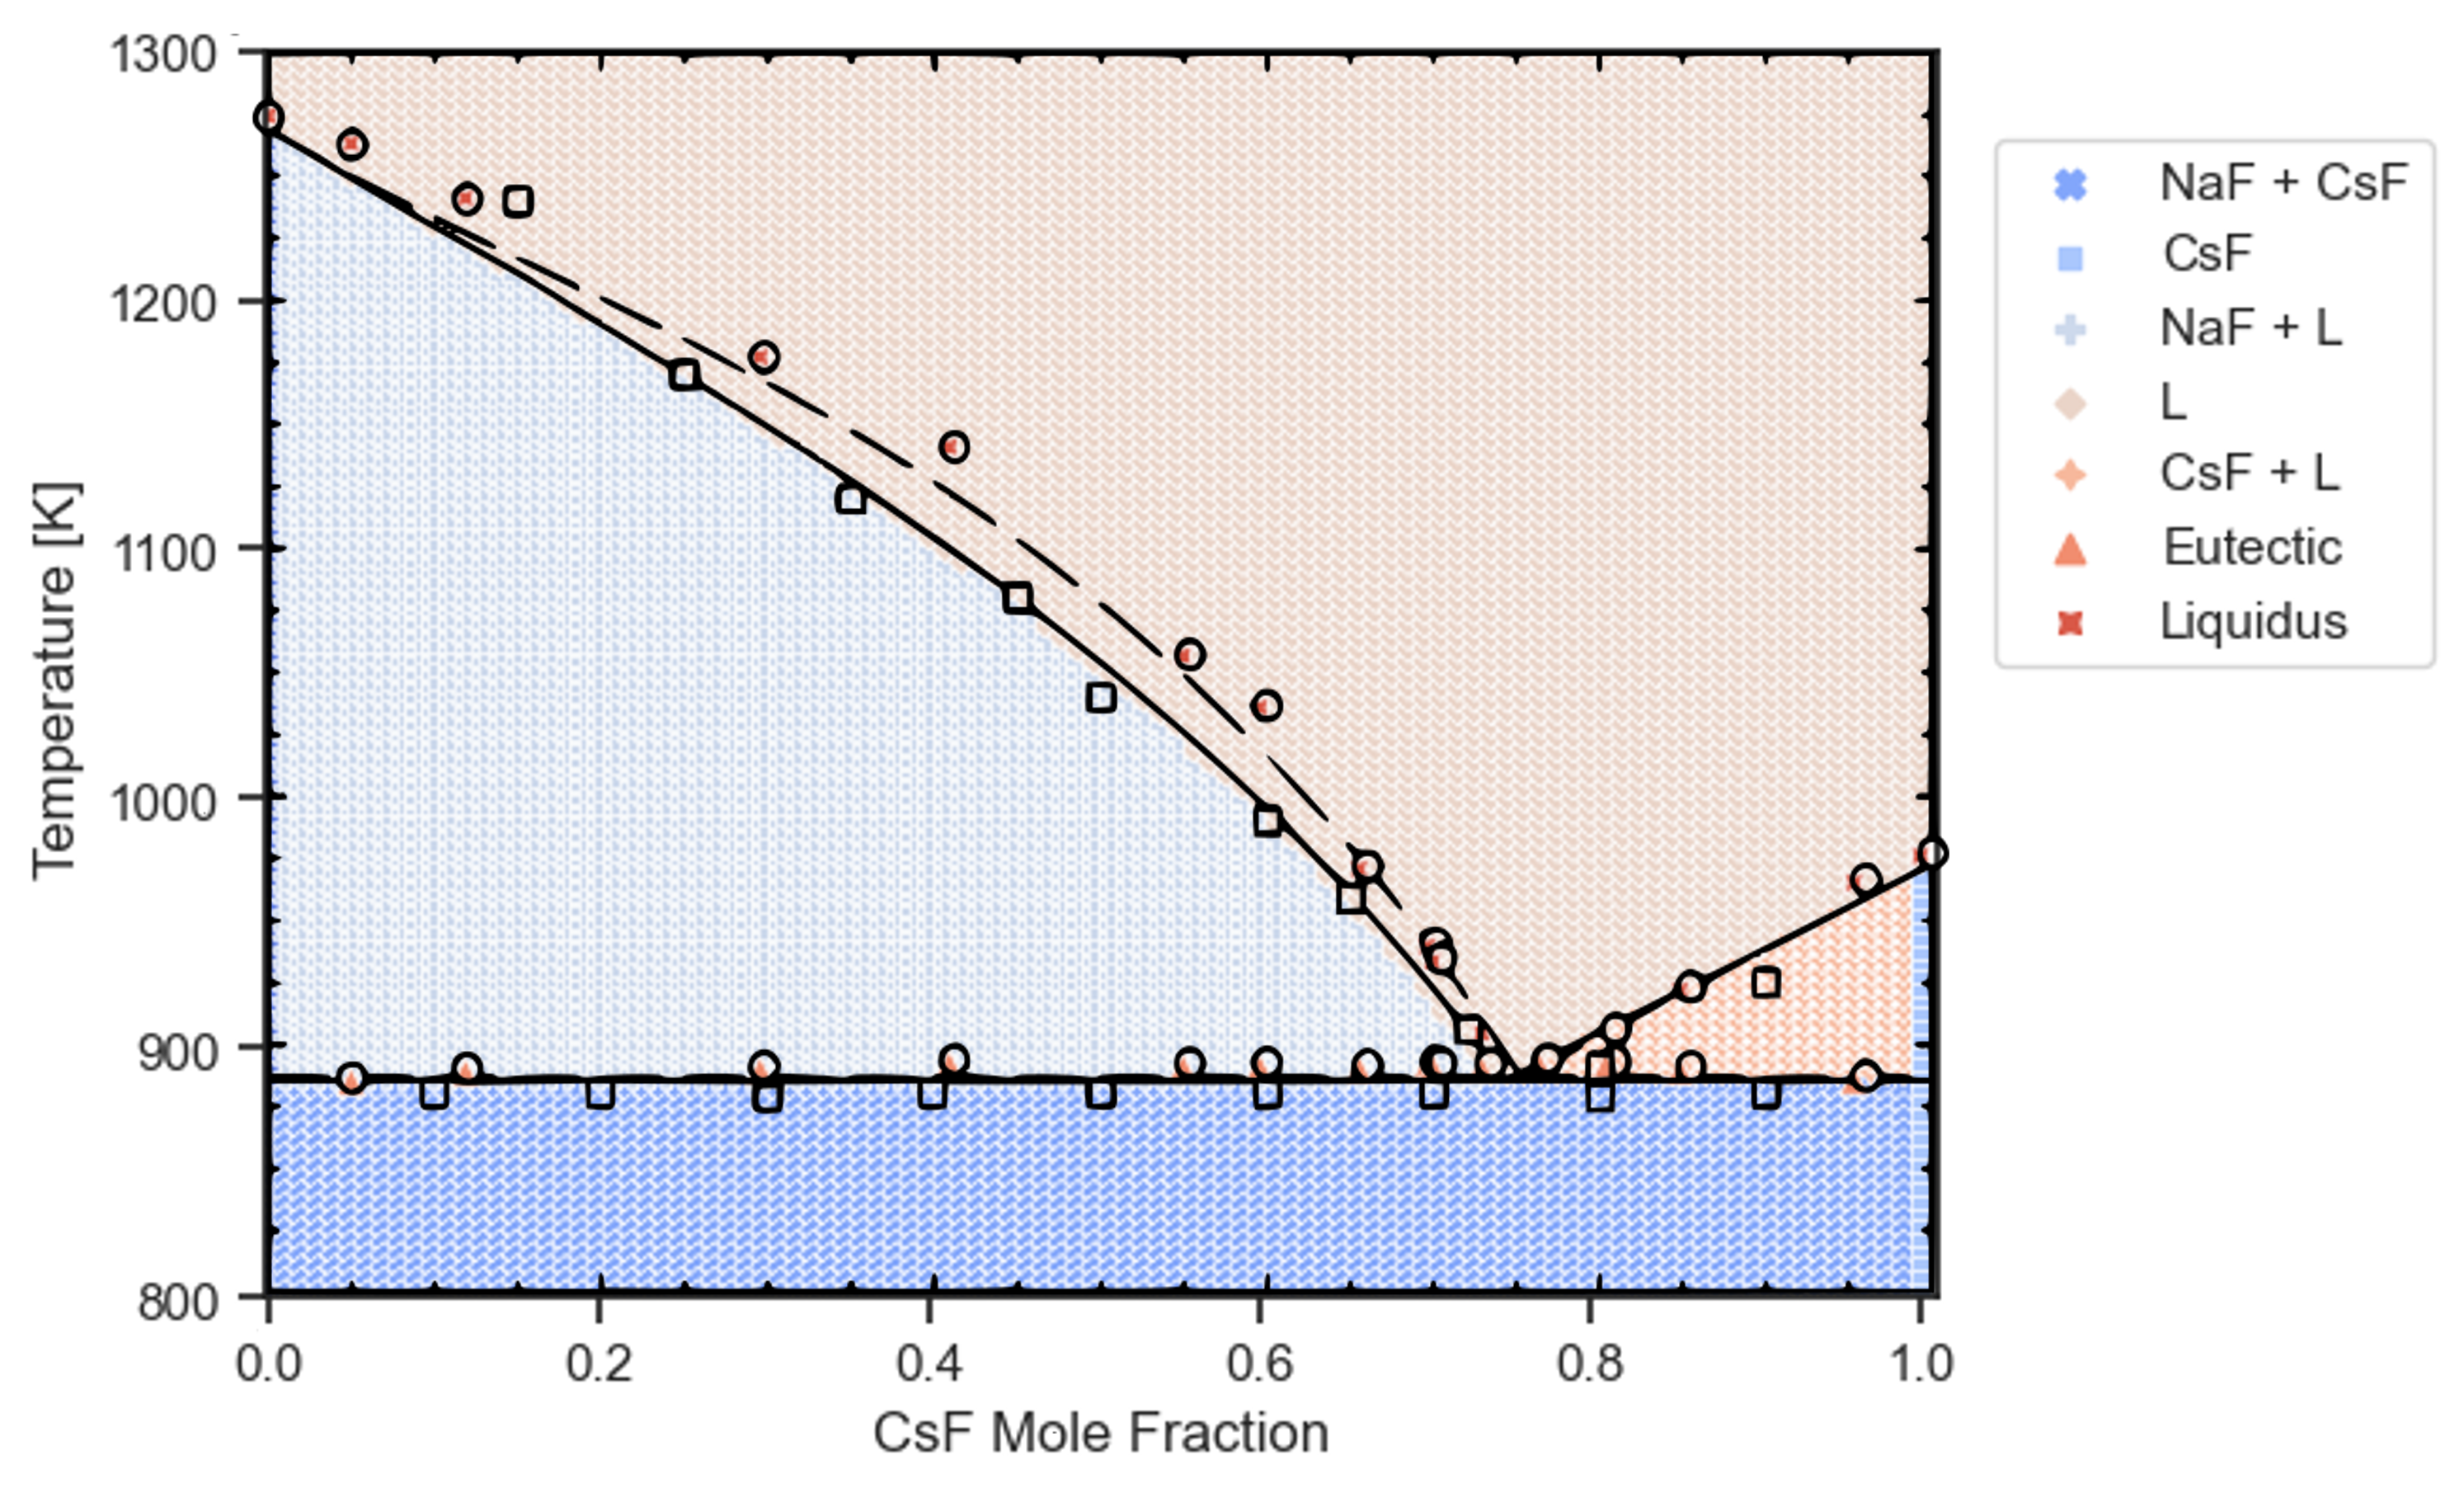
\includegraphics[width=0.95\textwidth]{figures/chapter-7/phasedia.png}
        \caption[Yellowjacket prediction of \ce{NaF-CsF} phase diagram.]{Yellowjacket prediction of \ce{NaF-CsF} phase diagram with the phase diagram from Lipkina et al. \cite{Lipkina:2022aa} overlayed on top.}
        \label{fig:res_phased}
    \end{figure}
    \begin{figure}
        \centering
        \includegraphics[width=0.7\textwidth]{figures/chapter-7/pdo.png}
        \caption[Reference \ce{NaF-CsF} phase  diagram from Lipkina et al.]{Reference \ce{NaF-CsF} phase  diagram from Lipkina et al. \cite{Lipkina:2022aa}.}
        \label{fig:res_refdia}
    \end{figure}
    There is, however, a departure between the liquidus points calculated by Lipkina et al. and the ones predicted by {\YJ}. This is a direct consequence of the database used in the calculations (MSTDB-TC) as it has not been updated to reflect the recent experimental results. In fact, as shown by the solid black line, the calculations match the results of the previously available experimental data. The example not only highlights the capability of {\GEM} but also shows a need for the re-evaluation of the \ce{NaF-CsF} thermodynamic model currently used in the databases.
    

\section{CANDU Fuel Phase Evolution}
Severe accident scenarios are amongst the phenomena that benefit most from the use of thermodynamic equilibrium calculations \cite{Piro:2021aa}. Piro performed thermodynamic investigations on irradiated uranium dioxide CANDU fuel under conditions representative of severe accident scenarios \cite{Piro:2022aa}. Piro considered two cases of irradiated fuel interacting with the atmosphere. In the first case, the fuel was in contact with hydrogen gas while in the second case the irradiated fuel was in contact with air and steam.  Piro used TAF-ID \cite{Gueneau15,Gueneau:2021aa} and varied the ratio of fuel to total atmospheric gas as well as the temperature and hydrostatic pressure. Here, a couple of similar simulations are performed albeit for the first case with a single fuel to atmosphere ratio and the database used is a modified version of TAF-ID obtained by translating the TAF-ID tdb file into ChemSage format. For the simulation, the same composition as that used by Piro was selected and the values are reported in Table~\ref{tab:composition_candu}. In the table, $b_{\ce{O}}$, $b_{\ce{H}}$ and $b_{\ce{N}}$ are variables which depend on the hydrogen to steam molar ratio $H = n_{\ce{H2}} / n_{\ce{H2O}}$, air to steam molar ratio $A = n_{\text{air}} / n_{\ce{H2O}}$, and fission product to atmosphere molar ratio $R = b_{\ce{Cs}} / n_{\text{gas}}$. The calculations show that under the given conditions, the main phase is O2ZRU\_C with other phases evolving as the system temperature changes. It must again be emphasised that the simulation is only representative of the capabilities developed as part of {\GEM} and must be considered as a safety case simulation. 
\begin{table}[htb]
		\centering
	   	\caption[Input mass parameters for CANDU fuel under severe accident condition.]{Input mass parameters for CANDU fuel under severe accident condition. Adopted from Piro \cite{Piro:2022aa}.}
	   	\begin{tabular}{@{} lcr @{}} % Column formatting, @{} suppresses leading/trailing space
	      		\toprule
	      		\textbf{Element} & \phantom{abc}& \textbf{Moles [\si{\mole}]} \\
	      		\midrule
	      		\ce{O}	& & $b_{\ce{O}}$\\
			\ce{U}	& & \num{1014.5}\\
			\ce{Np}	& & \num{0.096}\\
			\ce{Pu}	& & \num{2.754}\\
			\ce{Ce}	& & \num{0.824}\\
			\ce{Y}	& & \num{0.215}\\
			\ce{Te}	& & \num{0.138}\\
			\ce{La}	& & \num{0.332}\\
			\ce{Zr}	& & \num{1.442}\\
			\ce{Ba}	& & \num{0.389}\\
			\ce{Ru}	& & \num{0.899}\\
			\ce{Mo}	& & \num{1.15}\\
			\ce{Sr}	& & \num{0.421}\\
			\ce{I}		& & \num{0.077}\\
			\ce{Nd}	& & \num{0.859}\\
			\ce{Nb}	& & \num{0.043}\\
			\ce{Am}	& & \num{0.0064}\\
			\ce{Cs}	& & \num{0.745}\\
			\ce{Rh}	& & \num{0.166}\\
			\ce{H}	& & $b_{\ce{H}}$\\
			\ce{N} 	& & $b_{\ce{N}}$\\
	      		\bottomrule
	   \end{tabular}
	   \label{tab:composition_candu}
	\end{table}

Using $H = 10^5$ and $R = 10^{-4}$ for the case of fuel in contact with hydrogen, $b_{\ce{O}} = 2029.07449$ and $b_{\ce{H}} = 14900.00$. With the hydrostatic pressure $P = 1$ \si{\atmosphere}, the temperature of the system was varied from \SI{1000}{\kelvin} to \SI{3000}{\kelvin} in steps of \SI{50}{\kelvin}. The phase evolution predicted by {\GEM} is shown in Figure~\ref{fig:candu_phase}. One must note that the database used here is not TAF-ID so the results will be different from the ones predicted by Piro \cite{Piro:2022aa}.
\begin{figure}[ht]
         \centering
         \includegraphics[width=0.95\textwidth]{figures/chapter-7/Candu_moles.pdf}
         \caption{Predicted phase distribution with respect to temperature $H = 10^5$, $R = 10^{−4}$, and $P = 1$ \si{\atmosphere}.}
     \label{fig:candu_phase}
\end{figure}

In addition to comparing phase distributions under the varying system parameters, one is often interested in the oxidation states of different phases as they affect the material properties. Thermodynamic equilibrium calculations can be used to compute the oxygen-to-metal ratio $\left(O/M\right)$ of the phases. The same calculations as those used for the phase evolution were used to calculate the $\left(O/M\right)$ ratio and its evolution for O2ZRU\_C phase is shown in Figure~\ref{fig:candu_om}.
\begin{figure}[htb]
         \centering
         \includegraphics[width=0.7\textwidth]{figures/chapter-7/Candu_OM.pdf}
         \caption{Predicted oxygen-to-metal ratio $\left(O/M\right)$ for O2ZRU\_C phase with respect to temperature $H = 10^5$, $R = 10^{−4}$, and $P = 1$ \si{\atmosphere}.}
     \label{fig:candu_om}
\end{figure}

\section{Vapour Pressure Evolution in an MSR}
	Safety case demonstrations for MSRs are significantly different from water-cooled reactors. Since the fuel is already molten, there are no thresholds for a major release of radioactive material with severe core damage in MSR accidents. The consequences of a primary system breach depend on the size and breach location and how much of the fuel salt or fission gases are leaked into a confined space.  A small breach can result in significant fuel salt release and the high salt temperature can lead to a high pressure in the confined space  \cite{Holcomb:2021aa}. Predicting vapour pressures is important for such safety demonstrations, but also for design and development of off-gas treatment system. {\GEM} can predict the change of vapour pressure of elements in gas phase, which can be used in source-term analyses and other simulations.  The role of thermodynamic equilibrium solver in such cases can be demonstrated by the evolution of a fictive system representative of a molten salt system (\ce{FLiBe}) with some dissolved fissile material (\ce{U}) and some fission products (\ce{Nd, Ce, La, Cs, Rb}).  The system composition was adopted from Poschmann et al. \cite{Poschmann:2021ab} and is reported in Table~\ref{tab:composition_msr}.
	\begin{table}[htb]
		\centering
	   	\caption[Input mass parameters for MSR fuel vapour pressure evolution.]{Input mass parameters for MSR fuel vapour pressure evolution. From Poschmann et al. \cite{Poschmann:2021ab}.}
	   	\begin{tabular}{@{} lcr @{}} % Column formatting, @{} suppresses leading/trailing space
	      		\toprule
	      		\textbf{Element} & \phantom{abc}& \textbf{Moles [\si{\mole}]} \\
	      		\midrule
	      		\ce{Pu}	& & \num{1.9780d-1}\\
			\ce{U}	& & \num{9.9695d3}\\
			\ce{Nd}	& & \num{3.3553d-1}\\
			\ce{Ce}	& & \num{4.2081d-1}\\
			\ce{La}	& & \num{1.4912d-1}\\
			\ce{Cs}	& & \num{4.2326d-1}\\
			\ce{Rb}	& & \num{8.1960d-2}\\
			\ce{F}	& & \num{4.4d5}\\
			\ce{Be}	& & \num{1.0d5}\\
			\ce{Li} 	& & \num{2.0216d5}\\
	      		\bottomrule
	   \end{tabular}
	   \label{tab:composition_msr}
	\end{table}

    The system was assumed to undergo an unmitigated increase in temperature. The phase evolution, vapour pressure of species in gas phase and element potential change as a function of temperature are shown in figures~\ref{fig:res_molemsr}, \ref{fig:res_vpmsr} and \ref{fig:res_epmsr}.
        \begin{figure}[ht]
        \centering
        \includegraphics[width=0.9\textwidth]{figures/chapter-7/msr_moles.pdf}
        \caption{Phase evolution in molten salt system.}
        \label{fig:res_molemsr}
    \end{figure}
    \begin{figure}[ht]
        \centering
        \includegraphics[width=0.9\textwidth]{figures/chapter-7/msr_vp.pdf}
        \caption{Vapour pressure prediction in molten salt system.}
        \label{fig:res_vpmsr}
    \end{figure}
    \begin{figure}[ht]
        \centering
        \includegraphics[width=0.9\textwidth]{figures/chapter-7/msr_ep.pdf}
        \caption{Element potential evolution in MSR.}
        \label{fig:res_epmsr}
     \end{figure}
To reiterate, one must note that the results are purely for capability demonstration and must not be treated as physically relevant. However, they do exhibit cases where one might find the use of {\GEM} relevant.

\section{GEM - Phase Field Coupling}\label{sec:gem_pf}
The objective of {\YJ} development was to allow concurrent coupling of GEM with the phase field module in MOOSE. To achieve this a two step process was adopted. The first step was an offline coupling where {\GEM} calculations are used to pre-tabulate the Gibbs energy and chemical potential data. This data was then used to generate interpolated functions of Gibbs energy and chemical potentials using the \texttt{PiecewiseLinearInterpolationMaterial} object in MOOSE. The interpolated functions were used as material properties in the phase field calculation. In doing so, one must also account for the difference between the Gibbs energies required by the phase field model and those calculated by {\GEM}. The thermodynamic equilibrium calculations compute the Gibbs energy from the MQMQA and are in the following form given by equation~\eqref{EqGibbsMQM1}. On the other hand, the phase field model requires that the Gibbs energy and chemical potentials also capture the effect of redox reactions and hence the Gibbs energy in a phase field module takes the following form:
\begin{equation}
	g_\text{PF} = \sum x_i g_i^\text{ec}  + RT\left( \sum x_i \ln{x_i} \right) + g^\text{ex},
\end{equation}
where $g_i^\text{ec}$ denotes the Gibbs energy with the reduction component accounted for. 

For the initial demonstration of the methodology, \ce{LiF-NiF2} salt interacting with \ce{Ni} metal at \SI{1150}{\kelvin} was selected. The Gibbs energy from the thermodynamic equilibrium code then takes the following form:
\begin{equation*}
	g_\text{GEM} = x_{\ce{NiF2}} g_{\ce{NiF2}}^\circ + x_{\ce{LiF}} g_{\ce{LiF}}^\circ + RT\left( x_{\ce{NiF2}} \ln{x_{\ce{NiF2}}} + x_{\ce{LiF}} \ln{x_{\ce{LiF}}} \right) + g^\text{ex}.
\end{equation*}
To reduce the number of variables in the phase field model, the reference Gibbs energy of \ce{LiF2} is set to zero. Physically, since \ce{LiF} is not modelled, the energy should be based on the metallic form of \ce{Ni} which is done by changing the reference energy. \ce{NiF2} is assumed to be formed from \ce{Ni} metal by reducing   \ce{HF} into \ce{H2} and the Gibbs energy of formation of \ce{NiF2} is then equal to $g_{\ce{NiF2}}^\circ - 2 g_{\ce{HF}}^\circ + g_{\ce{H2}}^\circ + \nu F \Delta E_{\ce{F}}$. This gives the following Gibbs energy expression for the phase field model
\begin{equation*}
	g_\text{PF} = x_{\ce{NiF2}} \left( g_{\ce{NiF2}}^\circ - 2 g_{\ce{HF}}^\circ + g_{\ce{H2}}^\circ + \upsilon F \Delta E_{\ce{F}} \right) + RT\left( x_{\ce{NiF2}} \ln{x_{\ce{NiF2}}} + x_{\ce{LiF}} \ln{x_{\ce{LiF}}} \right) + g^\text{ex},
\end{equation*}
where $\upsilon$ represents the valency (2 for \ce{Ni^{2+}}), $F$ is Faraday's constant and $\Delta E_{\ce{F}}$ denotes the fluoride potential of the salt which is the energy required for the \ce{HF -> H2 + F^-} redox reaction. The fluoride potential is empirically derived based on experimental data and represents how oxidising the environment is (higher $\Delta E_{\ce{F}}$ is less oxidising). To use {\GEM} calculations in the phase field model, the Gibbs energy can then be reconciled as follows:
\begin{equation*}
	g_\text{PF} = g_\text{GEM} - x_{\ce{NiF2}} \left( 2 g_{\ce{HF}}^\circ - g_{\ce{H2}}^\circ - g_{\ce{LiF}}^\circ - \nu F \Delta E_{\ce{F}} \right).
\end{equation*}

A phase field simulation was performed by collaborators at the University of Florida\footnote{The phase field calculations were performed by Chaitanya Bhave, PhD candidate at the University of Florida.} to demonstrate the potential of coupling the Gibbs energy minimiser with the phase field model. The reference phase field model used the Nernst equation for the Gibbs energy equation, which does not capture the excess mixing contribution. As shown in Figure~\ref{fig:pfgibbs}, the use of GEM allowed capturing the excess mixing effects which were not captured previously. While the difference for the binary system considered was relatively small, the excess mixing contributions for larger systems such as ones with impurities can be significant and being able to capture the additional contributions can significantly improve the fidelity of phase field models.
    \begin{figure}[h!]
        \centering
        \includegraphics[width=0.75\textwidth]{figures/chapter-7/gibbs.png}
        \caption{Comparison of Gibbs energy predicted by {\GEM} vs. the dilute Nernst energy model used previously.}
        \label{fig:pfgibbs}
    \end{figure}

\ce{Ni} leaching with molten \ce{LiF-NiF2} was simulated under two conditions: $\Delta E_{\ce{F}} = 2.871$ \si{\volt}, which represents oxidising conditions and $\Delta E_{\ce{F}} = 3.0$ \si{\volt} which represents reducing conditions. The mole fraction of \ce{Ni} in the molten salt phase was fixed as $x_{\ce{Ni}} = 0.001$. This essentially makes the molten salt a large reservoir of \ce{Ni} and allows the corrosion of the structural material to be simulated without having to account for the mass inventory in the salt. The results of \ce{Ni} leaching have been shown in figures~\ref{fig:pfres2} and \ref{fig:pfres3}. Under oxidising conditions, \ce{Ni} metal gets leached into the molten salt and the interface moves to the left as shown in Figure~\ref{fig:pfres2} while the opposite happens under reducing conditions, as shown in  Figure~\ref{fig:pfres3}. 
\begin{figure}[!ht]
    \subfloat[Start of simulation\label{fig:EF2_i}]{%
      \includegraphics[width=0.475\textwidth]{figures/chapter-7/EF_2.871_i.pdf}
    }
    \hfill
    \subfloat[End of simulation\label{fig:EF2_e}]{%
      \includegraphics[width=0.475\textwidth]{figures/chapter-7/EF_2.871_e.pdf}
    }
    \caption[\ce{Ni} corrosion by \ce{LiF-NiF2} salt under oxidising condition $\left(\Delta E_{\ce{F}} = 2.871\right)$.]{Simulation of \ce{Ni} corrosion by \ce{LiF-NiF2} salt under oxidising condition $\left(\Delta E_{\ce{F}} = 2.871\right)$. Initially, the domain contained \ce{Ni} in the left half of the domain and molten salt in the right half as in subfigure (a). At the end of the simulation shown in subfigure (b), the oxidation of \ce{Ni} metal leads to the leaching of \ce{Ni} into the molten salt as exhibited by the interface shifting to the left (the dashed line denotes the initial position of interface).}
    \label{fig:pfres2}
\end{figure}

\begin{figure}[!ht]
    \subfloat[Start of simulation\label{fig:EF3_i}]{%
      \includegraphics[width=0.475\textwidth]{figures/chapter-7/EF_3.0_i.pdf}
    }
    \hfill
    \subfloat[End of simulation\label{fig:EF3_e}]{%
      \includegraphics[width=0.475\textwidth]{figures/chapter-7/EF_3.0_e.pdf}
    }
    \caption[\ce{Ni} corrosion by \ce{LiF-NiF2} salt under reducing condition $\left(\Delta E_{\ce{F}} = 3.0\right)$.]{Simulation of \ce{Ni} corrosion by \ce{LiF-NiF2} salt under reducing condition $\left(\Delta E_{\ce{F}} = 3.0\right)$. The initial interface is shown in subfigure (a) while at the end of the simulation shown in subfigure (b), the reduction of \ce{Ni} metal leads to gain of \ce{Ni} metal from the molten salt as exhibited by the interface shifting to the right (the dashed line denotes the initial position of interface).}
    \label{fig:pfres3}
\end{figure}

For the direct coupling of {\GEM} with the phase field module, the UserObject described in Chapter~\ref{chap:implementation} was developed. The UserObject allows a two way communication between the two parts of {\YJ} wherein the phase field code provides the state-space to the thermodynamic equilibrium solver which returns the Gibbs energy and chemical potentials of the species to the phase field code. The UserObject system is now being deployed to perform fully-coupled simulations.


\chapter{Conclusions} \label{chap:conclusions}

	Equilibrium thermodynamics provides the thermodynamic properties and driving forces for a wide variety of phenomena in nuclear reactors and a new equilibirium solver called {\GEM} has been developed. {\GEM} has been developed with the goal of enabling direct coupling of thermodynamic equilibrium calculations in multiphysics simulations performed using the Multiphysics Object Oriented Simulation Environment (MOOSE). Incorporating equilibrium calculations in multiphysics simulations comes with several challenges many of which are related to the existing software infrastructure. Though the most substantial contribution of this work is the creation of the software from ground up, several additional contributions were made to the field. First, while several algorithms from the literature are used, their implementation has a significant impact on the computational performance and this work had to be cognisant of this fact. The algorithms in the literature were modified to reflect the evolution in computing architectures. Second, despite model and database development being relatively mature, it was realised that knowledge gaps exist in the understanding of many models, such as the modified quasichemical model (MQM) and this work helped in improving the understanding of such models. Third, there is often a lack of understanding about the algorithms, their capabilities and limitations, and the interpretation of the results from equilibrium thermodynamics softwares and, through this work, an effort was made to clarify some these choices. Lastly, despite years of research into global optimisation algorithms, a majority of current equilibrium codes use a rather simplistic sampling approach that often leads to failure in converge or inaccurate results. This work used an approach based on numerical experiments to quantitatively compare some promising global optimisation approaches in terms of their applicability to the phase equilibria problem. 

	The development of the code was motivated by the need for a modelling tool for molten salt corrosion. Modelling corrosion requires understanding of the microstructure for which the phase field model is often used. The phase field model, in turn, requires several thermodynamic quantities which must be computed through an optimisation algorithm. Coupling with the phase field module of MOOSE was the primary goal for developing this code and the code must be able to handle several thermodynamic models used to describe such systems. The model most widely used for the molten salts is the Modified Quasichemical Model in Quadruplet Approximation (MQMQA) which wasn't very well understood previously. As part of this work, the MQMQA was analysed to get a better understanding and the chemical potential expressions were derived and published. Derivation of chemical potentials for non-ideal models is not trivial and most papers in open literature don't describe the models in sufficient details let alone giving the expressions of chemical potentials which can be implemented into code by software developers. The chemical potentials for some commonly used excess mixing models were shown in Chapter~\ref{chap:thermo}.
	
	Calculation of thermodynamic equilibrium is based on the fundamental laws of thermodynamics and several algorithms already reported in the literature were used to satisfy the necessary and sufficient conditions described in Chapter~\ref{chap:equilibrium}. The levelling method was used for initialisation followed by the full non-linear solution through the method of Lagrange multipliers. There are several factors that can impact the performance of the solver and the implementation of the code had to account for these factors. In doing so, the implementations were optimised to offer flexibility in terms of the system size, models that can be used, convergence criteria and others. Though the code cannot be presented herein due to export control restrictions, the algorithms used in the development were described in Chapter~\ref{chap:implementation} through flowcharts and the reasoning behind main design decisions were also justified. A major challenge in satisfying the sufficient condition of thermodynamic equilibrium is the need for global optimisation algorithms. This condition requires that the driving force of all metastable phases be positive but the driving force function is often non-convex for non-ideal models and ensuring that the driving force is indeed positive is not a straightforward task. Despite major advances in global optimisation methods, the applications to thermodynamic equilibrium have been few and are mostly limited to very simple problems such as vapour-liquid equilibrium. As part of this dissertation, significant effort was spent on performance considerations of global optimisation algorithms. The spatial branch \& bound (sBB) bound algorithm was experimentally compared with an adaptive particle swarm optimisation (APSO) to prove their applicability to the equilibrium problems. It was shown that compared to the often used grid sampling, both the selected algorithms show a higher reliability to cost ratio. While sBB had the highest reliability, it came at a computational cost. On the other hand, APSO showed a great compromise between cost and reliability and though it failed to converge a few times, it was usually noticeably faster than sBB. Since both algorithms have their pros and cons, justifying the choice of implementation depends on the application and therefore both the algorithms were implemented with the choice left to the end-user. Valuable insights into the performance of global optimisation algorithms was thus obtained and can help inform the decision of not only end-users but also of other developers.
	
	Though the work was aimed at developing capabilities rather than performing predictive calculations, several examples of potential applications were shown through demonstrations in Chapter~\ref{chap:results}. A simple coupling between the phase field and GEM code show how the fidelity of corrosion models may improve by adding equilibrium calculations. Moreover, the code will be a valuable tool in modelling other physical processes and in particular will be useful in source-term analyses and material modelling under non-normal operating conditions of nuclear reactors. To instil confidence in the accuracy of results predicted by the code, the results of {\GEM} were compared to the commercial code FactSage and excellent agreement was observed.
	
	In summary, the software developed as part of this work adds native thermodynamic equilibrium capability to the multiphysics simulation framework MOOSE. It would enable direct coupling of phase equilibrium calculations with other multiphysics codes in the MOOSE environment and allow modelling and simulation of complex physical phenomena helping in design and discovery of nuclear materials and help expedite the deployment of advanced reactors, in particular the molten salt reactor. The dissertation also addresses several knowledge gaps and concerns in the field of thermodynamic equilibrium modelling with the most significant being a better understanding of the MQMQA and a rigorous experimental comparison of methods for global optimisation applied to phase equilibrium calculations.
	
	
	
\chapter{Recommendations} \label{chap:future}
	Several improvements can be made to the software to extend the range of applications and to enhance the computational performance. Currently, explicit expressions of Gibbs energy and chemical potential are required for each model. Implementing the pre-derived expressions allows reducing the computational expenses but also has a number of limitations. First, not-only is significant effort is required to implement new models but doing so can inevitably introduce typographical errors creating bugs which might be tedious to debug. Second, every time a new derivative is required, such as with respect to temperature to calculate heat capacity, the user or developer must invest significant time. With automatic differentiation methods maturing, their impact on performance has significantly reduced and their implementation is not as big an impediment as it was until a few years ago. Using MetaPhysicL \cite{Lindsay:2021aa}, these disadvantages of hard-coded expressions can be overcome and by strategically invoking this capability, negligible performance impact can be achieved. Another recommendation is efforts to reduce the computational cost of equilibrium calculations. There is a foreseeable advantage in improving the initialisation strategy and one such effort has been partly tried in this work. This idea is based on caching the previous calculations and using the nearest previous calculation to initialise a new calculation. Each calculation can be indexed as nodes of a $k$-dimensional tree ($k$-d tree) and the strategy has already been implemented in MOOSE albeit not tested for {\GEM} despite the data-structures being designed for such application. Though one must consider the impact on memory requirements and search time, this strategy is promising and should be tested and fully implemented in \GEM. There's also a potential on further improving global optimisation algorithms. The convergence of sBB may be significantly improved by implementing heuristics and improved bound tightening strategies specific to the nature of the problem explored here. Similarly, further optimising the hyper-parameters used in APSO may allow improvements to both its performance and reliability helping improve the performance of {\GEM} as well.
	
	In terms of real applications, the code may benefit with the addition of several other models which are often used in modelling nuclear materials. The magnetic contribution to Gibbs energies was neglected in this work. Also, less-frequently used models such as the sub-ionic liquid model (SUBI) were not implemented. Implementing these models will allow much broader applications of code. In the same light, implementation of parsing capability for ThermoCalc format (*.tdb) data files might be of interest since many databases, like TAF-ID, are often only available in this format and the tools for converting one format to another are still nascent and bug-riddled. Despite the best attempts at reducing the computational cost of equilibrium calculations, they are inherently expensive and can often impede and even prohibit any real-world simulation. Several strategies can be considered with the goal of accelerating equilibrium calculations in multiphysics simulations. The most promising and simplest to implement would be using the previously mentioned $k$-d tree to interpolate the results in regions with high confidence without running a full equilibrium calculations. As an example, if a new composition lies in a solution phase region, its properties can be estimated reasonably well with lever rule, saving the computational cost. In doing so, one may even look at more advanced strategies such as use of surrogate models.
	
	Though, the code developed as part of this work is a significant contribution as it is, the potential of growth is significant and some of the most promising applications might only be explored in future. Implementing some of the recommendation will vastly improve the performance and capability of the equilibrium code and allow it to achieve a lot more than it already can.

\references{dissertation.bib}

%% Use letters for the chapter numbers of the appendices.
\appendix

%% Turn off thumb indices for unnumbered chapters.
%\thumbfalse

% \include{cv/cv}
\chapter*{List of Publications}
\addcontentsline{toc}{chapter}{List of Publications}
\setheader{List of Publications}
\label{publications}

%% We use the 'etaremune' environment (the reverse of 'enumerate') to get a
%% numbered list of publications in reverse chronological order. If the list of
%% authors is long, it might be useful to emphasize your own name with \textbf.
\begin{enumerate}{\small
\item {M.\ Piro}, {M.\ Poschmann} and \textbf{P.\ Bajpai}, \textit{On the interpretation of chemical potentials computed from equilibrium thermodynamic codes: Applications to molten salts}, \href{https://doi.org/10.1016/j.jnucmat.2019.151756}{Journal of Nuclear Materials, 526 (2019) 151756}.
\item \textbf{P.\ Bajpai}, {M.\ Poschmann}, {M.\ Piro}, \textit{Derivations of useful partial molar excess Gibbs energy of mixing expressions of common thermodynamic models}, To be submitted to \href{https://www.journals.elsevier.com/calphad}{CALPHAD Computer Coupling of Phase Diagrams and Thermochemistry}. [In preparation]
\item \textbf{P.\ Bajpai}, {M.\ Poschmann}, {D.\ Andr\v{s}}, {C.\ Bhave}, {M.\ Tonks} and {M.\ Piro}, \textit{Development of a new thermochemistry solver for multiphysics simulations of nuclear materials}, \href{http://https://www.tms.org/TMS2020}{TMS 2020 Supplemental Proceedings, TMS 2020  - 149\textsuperscript{th} Annual Meeting \& Exhibition, San Diego, February 23-27, 2020}. [Accepted]
\item \textbf{P.\ Bajpai}, {M.\ Poschmann}, {D.\ Andr\v{s}} and {M.\ Piro}, \textit{Progress in developing a new thermochemistry code for corrosion modelling and multiphysics simulation of nuclear fuels}, \href{http://cns-annual-conference.org/2019/index.html}{39\textsuperscript{th} Annual Conference of the Canadian Nuclear Society and 43\textsuperscript{rd} Annual CNS/CNA Student Conference, Ottawa, June 23-26, 2019}.
}\end{enumerate}

\setboolean{@twoside}{false}

\newpage
\dedication{{M.\ Piro}, {M.\ Poschmann} and \textbf{P.\ Bajpai} \\ \textit{On the interpretation of chemical potentials computed from equilibrium thermodynamic codes: Applications to molten salts}\\ \href{https://doi.org/10.1016/j.jnucmat.2019.151756}{Journal of Nuclear Materials, 526 (2019) 151756}.}

\includepdf[pages=-]{publications/Piro_JNM_2019.pdf}

\newpage
\dedication{\textbf{P.\ Bajpai}, {M.\ Poschmann} and {M.\ Piro}\\ \textit{erivations of useful partial molar excess Gibbs energy of mixing expressions of common thermodynamic models}\\ To be submitted to \href{https://www.journals.elsevier.com/calphad}{CALPHAD Computer Coupling of Phase Diagrams and Thermochemistry}. [In preparation]}

\includepdf[pages=-]{publications/Bajpai_Calphad_2020.pdf}

\newpage
\dedication{\textbf{P.\ Bajpai}, {M.\ Poschmann}, {D.\ Andr\v{s}}, {C.\ Bhave}, {M.\ Tonks} and {M.\ Piro}\\ \textit{Development of a new thermochemistry solver for multiphysics simulations of nuclear materials}\\ \href{http://https://www.tms.org/TMS2020}{TMS 2020 Supplemental Proceedings, TMS 2020  - 149\textsuperscript{th} Annual Meeting \& Exhibition, San Diego, February 23-27, 2020}. [Accepted]}
\includepdf[pages=-]{publications/Bajpai_TMS_2020.pdf}


\setboolean{@twoside}{false}

\newpage
\dedication{
\textbf{P.\ Bajpai}, {M.\ Poschmann}, {D.\ Andr\v{s}} and {M.\ Piro}\\ \textit{Progress in developing a new thermochemistry code for corrosion modelling and multiphysics simulation of nuclear fuels}\\ \href{http://cns-annual-conference.org/2019/index.html}{39\textsuperscript{th} Annual Conference of the Canadian Nuclear Society and 43\textsuperscript{rd} Annual CNS/CNA Student Conference, Ottawa, June 23-26, 2019}.}
\includepdf[pages=-]{publications/CNS_Poster.pdf}
\includepdf[pages=-]{publications/Bajpai_CNS_2019.pdf}

\setboolean{@twoside}{false}


\end{document}

